\documentclass[
a4paper,                        % paper size
11pt,                           % font size
twoside,                        % two sided
footsepline,                    % add a line to separate the footer
headsepline,                    % add a line to separate the header
headexclude,                    % header does not belong to the text
footexclude,                    % footer does not belong to the text
pagesize,                       % set the pagesize in a DVI document
bibtotocnumbered,               % add the bibliography to the TOC
idxtotoc                        % add the index to the TOC
%openright,                      % start a new chapter on the right page
%,DIV12
%,draft
]{scrreprt}

\usepackage[draft]{varioref}    % defines \vref
\usepackage{hyperref}                      % automatically creates links when
                                % using pdflatex, defines \url
\usepackage{ifpdf}              % defines \ifpdf
\usepackage{graphicx}           % handles graphics
\usepackage{makeidx}            % creates the index
\usepackage{color}              % use colors

\usepackage{amsmath}

\usepackage{verbatim}           % required for \verbatim and \endverbatim
\usepackage{fancyvrb}
\usepackage{tocloft}            % required for the quickref
\usepackage{calc}               % compute length
\usepackage{ifthen}             % provide ifthen
\usepackage{xspace}
\usepackage{units}
\usepackage[numbers]{natbib}

% Make '_' a normal character (from http://www.tug.org/TeXnik/mainFAQ.cgi)
\usepackage{underscore}
% \begingroup
%   \lccode`\~=`\_
% \lowercase{\endgroup
%   \pdfstringdefDisableCommands{\let~\relax}%
% }
%%%%%%%%%%%%%%%%%%%%%%%%%%%%%%%%%%%%%%%%%%%%%%%%%%
%%%%%%%%%%%%%%%%%%%%%%%%%%%%%%%%%%%%%%%%%%%%%%%%%%
%%%%%%%%% New Commands and Environments %%%%%%%%%%
%%%%%%%%%%%%%%%%%%%%%%%%%%%%%%%%%%%%%%%%%%%%%%%%%%
%%%%%%%%%%%%%%%%%%%%%%%%%%%%%%%%%%%%%%%%%%%%%%%%%%
\newcommand{\es}{\mbox{\textsf{ESPResSo}}\xspace}
\newcommand{\ie}{\textit{i.e.}\xspace}
\newcommand{\eg}{\textit{e.g.}\xspace}
\newcommand{\etal}{\textit{et al.}\xspace}

\newcommand{\codebox}[1]%
{\texttt{#1}}

\DefineVerbatimEnvironment{code}{Verbatim}%
{commandchars=\\\{\}}
\makeatletter
\newenvironment{tclcode}
{%
  \addtolength{\linewidth}{-2em}% set the line length
  \@minipagetrue%%%DPC%%%
  \@tempswatrue%%%DPC%%%
  \hsize=\linewidth%
  \setbox0=\vbox\bgroup\verbatim
}{\endverbatim
  \unskip\setbox0=\lastbox%%%DPC%%%
  \egroup
  \par%
  \noindent\hspace{1em}%
  \codebox{\box0}%
  \par\noindent%
}
\makeatother

% required so that we can set index numbers bold
% \index{Some example|mainindex}
\newcommand*{\mainindex}[1]{\textbf{\hyperpage{#1}}}

\newcommand{\todo}[1]{
  \marginpar{%
    \setlength{\fboxrule}{1pt}
    \fcolorbox{red}{yellow}{%
      \parbox{\marginparwidth-2\fboxrule-2\fboxsep}{%
        \bf\raggedright\scriptsize #1%
      }%
    }%
  }%
}

\makeatletter
\renewcommand{\minisec}[1]{\@afterindentfalse \vskip 1.5ex
  {\parindent \z@
    \raggedsection\normalfont\sffamily\itshape\nobreak#1\par\nobreak}%
  \@afterheading}
\makeatother

%%%%%%%%%%%%%% Syntax Description %%%%%%%%%%%%%%%

%%%%%% SYNTAX DEFINITION LAYOUT
%% Defines environments and commands to be used when defining the
%% syntax of a Tcl command.
% typesetting inside a command definition
% keywords/literals
\newcommand{\lit}[1]{\mbox{\texttt{#1}}}
\newcommand{\keyword}[1]{\mbox{\texttt{#1}}}
% variables
\newcommand{\var}[1]{\ensuremath{\mathrm{\mathit{#1}}}}
% option
\newcommand{\opt}[1]{\mbox{\textrm{[}#1\textrm{]}}}
\newcommand{\optlong}[1]{\textrm{[}#1\textrm{]}}
% alternatives
\newcommand{\alt}[1]{\textrm{(} #1 \textrm{)}}
\newcommand{\asep}{$|$\xspace}
% variant
% \rawvariant is required, as the command is changed during the
% essyntax environment
\newcommand{\rawvariant}[1]{\mbox{\textnormal{(#1)}}\xspace}
\newcommand{\variant}[1]{\rawvariant{#1}}
\newcommand{\fmark}[1]{%
  \raisebox{1ex}{%
    \textrm{\footnotesize #1}%
  }%
}
% feature
\newcommand{\feature}[1]{\texttt{\MakeUppercase{#1}}}

\newcommand{\require}[2]{%
  \mbox{#2\,\fmark{#1}}%
}
\newcommand{\required}[2][]{%
  \ifthenelse{\equal{#1}{}}{#2}{%
    \mbox{\fmark{#1}\,\feature{#2}}%
  }
}
\newenvironment{features}{%
  \par\smallskip%
  \small%
  \textrm{Required\hspace{1ex}features:}%
  \raggedright%
}{}

%% Layout thesyntax description box
\newsavebox{\theessyntaxbox}
\newlength{\essyntaxboxheight}
\newlength{\essyntaxboxdepth}
\newenvironment{essyntaxbox}{%
  \par\noindent%
 \begin{lrbox}{\theessyntaxbox}%
   \begin{minipage}{\linewidth-5em}%
     \ttfamily%
     \setlength{\parindent}{-3em}%
   }{%
   \end{minipage}%
 \end{lrbox}%
 \settoheight{\essyntaxboxheight}{\usebox{\theessyntaxbox}}%
 \settodepth{\essyntaxboxdepth}{\usebox{\theessyntaxbox}}%
 \hspace{1.5em}%
 \rule[-\essyntaxboxdepth]{1pt}{\essyntaxboxheight+\essyntaxboxdepth}%
 \hspace{3.5em}%
 \usebox{\theessyntaxbox}%
}

%% Environment for syntax descriptions
\newcounter{essyntaxcounter}
\setcounter{essyntaxcounter}{0}
\newenvironment{essyntax}{%
  \stepcounter{essyntaxcounter}%
  \label{essyntax:\arabic{essyntaxcounter}}
  % Create headings
  \minisec{Syntax}\nopagebreak%
  \smallskip\nopagebreak%
  \renewcommand{\variant}[1]{\par\rawvariant{##1}}
  \begin{essyntaxbox}%
  }{%
  \end{essyntaxbox}%
  \renewcommand{\variant}[1]{\rawvariant{##1}}
  \minisec{Description}%
}
% Define the starred environment (identical to unstarred, only it is
% not copied to the Quick reference)
\newenvironment{essyntax*}{\essyntax}{\endessyntax}

%% List-environment for the description of the arguments of a command
\newenvironment{arguments}{
  \minisec{Arguments}
  \begin{list}{}{
      \setlength{\rightmargin}{1em}
      \setlength{\leftmargin}{2em}
      \setlength{\partopsep}{0pt}
      \setlength{\topsep}{1ex}
      \setlength{\parsep}{0.5ex}
      \setlength{\listparindent}{-1em}
      \setlength{\labelwidth}{0.5em}
      \setlength{\labelsep}{0.5em}
      \renewcommand{\makelabel}[1]{\textbullet\,\texttt{##1}}
    }
  }{
  \end{list}
}

%%%%%%%%%%%%%%%%%%%%%%%%%%%%%%%%%%%%%%%%%%%%%%%%%%
%%% Declare new features/commands/analyze subcommands
%%%%%%%%%%%%%%%%%%%%%%%%%%%%%%%%%%%%%%%%%%%%%%%%%%
% Feature declaration
\newcommand{\newfeature}[1]{%
  \index{features!{\scriptsize #1}|mainindex}%
  \hypertarget{#1}{\texttt{\textbf{#1}}}%
}

% Create label and index entries for an Espresso tcl command
\newcommand{\newescommand}[2][NONE]{%
  \ifthenelse{\equal{#1}{NONE}}%
  {\label{tcl:#2}}%
  {\label{tcl:#1}}%
  \index{#2@\texttt{#2} (Tcl-command)|mainindex}%
  \index{Tcl-commands!#2@\texttt{#2}|mainindex}%
}

% Create index entries for analysis functions
\newcommand{\analyzeindex}[1]{%
  \index{#1|mainindex}%
  \index{analysis!#1|mainindex}%
}

%%%%%%%%%%%%%%%%%%%%%%%%%%%%%%%%%%%%%%%%%%%%%%%%%%
%%%%%%%%%%%%%%%%%%%%%%%%%%%%%%%%%%%%%%%%%%%%%%%%%%
%%%%%%%%%%%%%%%% Other Settings %%%%%%%%%%%%%%%%%%
%%%%%%%%%%%%%%%%%%%%%%%%%%%%%%%%%%%%%%%%%%%%%%%%%%
%%%%%%%%%%%%%%%%%%%%%%%%%%%%%%%%%%%%%%%%%%%%%%%%%%
\makeindex

%%%%%%%%%%%%%%%%%%%%%%%%%%%%%%%%%%%%%%%%%%%%%%%%%%
%%%%%%%%%%%%%%%%%%%%%%%%%%%%%%%%%%%%%%%%%%%%%%%%%%
%%%%%%%%%%%%%%%%% Main Document %%%%%%%%%%%%%%%%%%
%%%%%%%%%%%%%%%%%%%%%%%%%%%%%%%%%%%%%%%%%%%%%%%%%%
%%%%%%%%%%%%%%%%%%%%%%%%%%%%%%%%%%%%%%%%%%%%%%%%%%
\begin{document}
\titlehead{
  \begin{center}
    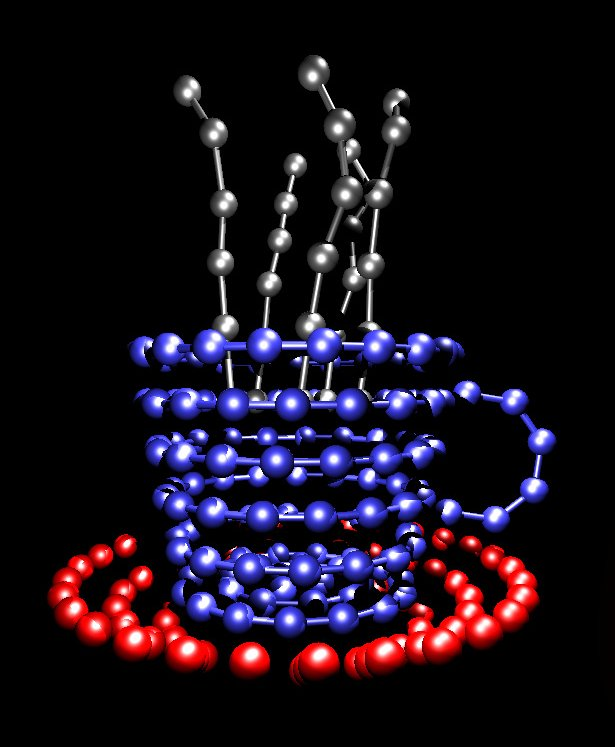
\includegraphics[width=5cm]{figures/logo}
  \end{center}
}
%\subject{}
\title{\es{} User's Guide}
%\author{}
%\date{\today}
\maketitle

\pdfbookmark{Contents}{toc}
\tableofcontents

\chapter{Introduction}
\label{chap:intro}

\todo{Make the following lists full text.}

\begin{itemize}
\item \es{} is a generic soft matter simulation packages
\item for molecular dynamics simulations in soft matter research
\item focussed on coarse-grained models
\item employs modern algorithms (Lattice-Boltzmann, DPD, P3M, \ldots)
\item written in C for maximal portability
\item Tcl-controlled
\item parallelized
\end{itemize}

\section{Guiding principles}
\label{sec:ideas}

(from paper: 2.1 Goals and principles)

\es
\begin{itemize}
\item does \emph{not} do the physics for you!
\item requires you to understand what you do (can not be used as a
  black box)
\item gives you maximal freedom (flexibility)
\item is extensible
\item integrates system setup, simulation and analysis, as this can't
  be strictly separated in soft matter simulations
\item has no predefined units
\item sets as few defaults as possible
\end{itemize}

\section{Algorithms contained in \es}

The following algorithms are implemented in \es{}:

\begin{itemize}
\item ensembles: NVE, NVT, NpT
\item charged systems:
  \begin{itemize}
  \item P3M for fully periodic systems
  \item ELC and MMM-family of algorithms for charged systems with
    non-periodic boundary conditions
  \item Maggs algorithm 
  \end{itemize}
\item Hydrodynamics:
  \begin{itemize}
  \item DPD (as a thermostat)
  \item Lattice-Boltzmann
  \end{itemize}
\end{itemize}

\section{Basic program structure}
\label{sec:structure}

(from paper: 2.2 Basic program structure)

\begin{itemize}
\item Control level: \texttt{Tcl}
\item ``Kernel'' written in \texttt{C}
\item This user's guide will focus on the control level
\end{itemize}

\section{On units}
\label{sec:units}
\index{units}
\index{length unit}
\index{time unit}
\index{energy unit}
\index{physical units}

What is probably one of the most confusing subjects for beginners of
\es is, that \es does not predefine any units.  While most MD programs
specify a set of units, like, for example, that all lengths are
measured in \AA ngstr\"om or nanometers, times are measured in nano- or
picoseconds and energies are measured in $\frac{kJ}{\mathrm{mol}}$,
\es does not do so.

Instead, the length-, time- and energy scales can be freely chosen by
the user.  A length of $1.0$ can mean a nanometer, an \AA ngstr\"om,
or a kilometer - depending on the physical system, that the user has
in mind when he writes his \es-script.  The user can choose the unit
system that suits the system best.

When creating particles that are intended to represent a specific type
of atoms, one will probably use a length scale of \AA ngstr\"om.  This
would mean, that \eg the parameter $\sigma$ of the Lennard-Jones
interaction between two atoms would be set to twice the van-der-Waals
radius of the atom in \AA ngstr\"om.  Alternatively, one could set
$\sigma$ to $2.0$ and measure all lengths in multiples of the
van-der-Waals radius.

The second choice to be made is the energy (and time-) scale.  One can
for example choose to set the Lennard-Jones parameter $\epsilon$ to
the energy in $\frac{kJ}{\mathrm{mol}}$.  Then all energies will be
measured in that unit.  Alternatively, one can choose to set it to
$1.0$ and measure everything in multiples of the van-der-Waals binding
energy.

As long as one remains within the same unit system throughout the
whole \es-script, there should be no problems.

\section{Requirements}
\label{sec:requirements}
\index{requirements}

The following libraries and tools are required to be able to compile
and use \es:

\begin{description}
\item[Tcl/Tk] \index{Tcl/Tk} \es{} requires the Toolkit Command
  Language Tcl/Tk \footnote{\url{http://www.tcl.tk/}} in the version
  8.3 or later.  Some example scripts will only work with Tcl 8.4. You
  do not only need the interpreter, but also the header files and
  libraries.  Depending on the operating system, these may come in
  separate development packages. If you want to use a graphical user
  interface (GUI) for your simulation scripts, you will also need Tk.
  
\item[FFTW] \index{FFTW} In addition, \es{} needs the FFTW library
  \footnote{\url{http://www.fftw.org/}} for Fourier transforms.
  ESPResSo can work with both the 2.1.x and 3.0.x series. Again, the
  header files are required.
  
\item[MPI] \index{MPI} Finally, if you want to use \es{} in parallel,
  you need a working MPI environment (version 1.2). Currently, the
  following MPI implementations are supported:
  \begin{itemize}
  \item LAM/MPI is the preferred variant
  \item MPICH, which seems to be considerably slower than LAM/MPI in
    our benchmarks.
  \item On AIX systems, \es{} can also use the native POE parallel
    environment.
  \item On DEC/Compaq/HP OSF/Tru64, \es{} can also use the native
    dmpirun MPI environment.
  \end{itemize}
\end{description}


\section{Syntax description}
\label{sec:syntax}


Throughout the user's guide, formal definitions of the syntax of
several Tcl-commands can be found. The following conventions are used
in these decriptions:
\begin{itemize}
\item Different \emph{variants} of a command are labelled \variant{1},
  \variant{2}, \ldots
\item Keywords and literals of the command that have to be typed
  exactly as given are written in \lit{typewriter} font.
\item If the command has variable arguments, they are set in
  \var{italic font}. The description following the syntax definition
  should contain a detailed explanation of the argument and its
  type.
\item \texttt{\alt{\var{alt1} \asep \var{alt2}}} specifies, that one
  of the alternatives \var{alt1} or \var{alt2} can be used.
\item \texttt{\opt{\var{argument}}} specifies, that the arugment
  \var{argument} is optional, \ie{} it can be omitted.
\item When an optional argument or a whole command is marked by a
  superscript label (\fmark{1}), this denotes that the argument can
  only be used, when the corresponding feature (see appendix
  \vref{chap:features}) specified in ``Required features'' is
  activated.
\end{itemize}


\minisec{Example}

\renewcommand{\variant}[1]{\par\rawvariant{#1}}
\begin{essyntaxbox}
  \variant{1} 
  constraint wall normal \var{n_x} \var{n_y} \var{n_z} 
  dist \var{d} type \var{id}
  
  \variant{2}
  constraint sphere center \var{c_x} \var{c_y} \var{c_z} 
  radius \var{rad} direction \var{direction} type \var{id} 
  
  \require{1}{%
    \variant{3}
    constraint rod center \var{c_x} \var{c_y} 
    lambda \var{lambda}
  } 
  
  \require{2,3}{%
    \variant{4}
    constraint ext_magn_field \var{f_x} \var{f_y} \var{f_z} 
  }

  \begin{features}
    \required{CONSTRAINTS}
    \required[1]{ELECTROSTATICS}
    \required[2]{ROTATION}
    \required[3]{DIPOLES}
  \end{features}

\end{essyntaxbox}
\renewcommand{\variant}[1]{\rawvariant{#1}}

%%% Local Variables: 
%%% mode: latex
%%% TeX-master: "ug"
%%% End: 


\chapter{First steps}
\label{chap:firststeps}

\section{Quick installation}

\index{configure}\index{make}

If you have the requirements (see section \vref{sec:requirements})
installed, in many cases, to compile \es{}, it is enough to execute
the following sequence of two steps in the directory where you have
unpacked the sources:
\begin{code}
configure
make
\end{code}

\todo{Mention minimal configuration without myconfig.h}
In some cases, \eg{} when \es{} needs to be compiled for several
different platforms or when different versions with different sets of
features are required, it might be useful to execute the commands not
in the source directory itself, but to start \texttt{configure} from
another directory (see section \vref{sec:builddir}). Furthermore, many
features of \es{} can be selectively turned on or off in the local
configuration header of \es{} (see section \vref{sec:myconfig}) before
starting the compilation with \texttt{make}.

The shell script \texttt{configure} prepares the source code for
compilation. It will determine how to use and where to find the
different libraries and tools required by the compilation process, and
it will test what compiler flags are to be used.  The script will find
out most of these things automatically.  If something is missing, it
will complain and give hints how to solve the problem.  The
configuration process can be controlled with the help of a number of
options that are explained in section \vref{sec:configure}.

The command \texttt{make} will compile the source code. Depending on
the options passed to the program, \texttt{make} can also be used for
a number of other things:
\begin{itemize}
\item It can install and uninstall the program to some other
  directories. However, normally it is not necessary to actually
  \textit{install} \es{} to run it.
\item It can test the \es{} program for correctness.
\item It can build the documentation.
\end{itemize}
The details of the usage of \texttt{make} are described in section
\vref{sec:make}.

When these steps have successfully completed, \es{} can be started
with the command (see section \vref{sec:run})
\begin{code}
Espresso
\end{code}

\section{Running \es}

\footnote{\url{http://www.tcl.tk/man/tcl8.5/tutorial/tcltutorial.html}}

\es{} is implemented as an extension to the Tcl script language. This means that you need to write a
script for any task you want to perform with \es. To learn about the Tcl script language and
especially the \es{} extensions, this chapter offers two tutorial scripts. The first will guide you
step by step through creating your first simulation script, while the second script is a well
documented example simulation script. Since the latter is slightly more complex and uses more
advanced features of \es{}, we recommend to work through both scripts in the presented order.

\section{Creating the first simulation script}

This section introduces some of the features of \es\ by
constructing step by step a simulation script for a simple salt crystal.
We cannot give a full Tcl tutorial here; however, most of the constructs
should be self--explanatory. We also assume that the reader is familiar with the
basic concepts of a MD simulation here. The code pieces can be copied step by
step into a file, which then can be run using \verb|Espresso <file>| from the
\es source directory.

Our script starts with setting up the initial configuration.  Most conveniently,
one would like to specify the density and the number of particles of the system
as parameters:
\begin{tclcode}
set n_part 200; set density 0.7
set box_l [expr pow($n_part/$density,1./3.)]
\end{tclcode}
These variables do not change anything in the simulation engine, but are just
standard Tcl variables; they are used to increase the readability and
flexibility of the script. The box length is not a parameter of this simulation;
it is calculated from the number of particles and the system density. This
allows to change the parameters later easily, e.~g.\ to simulate a bigger
system.

The parameters of the simulation engine are modified by the \verb|setmd|
command. For example
\begin{tclcode}
setmd box_l $box_l $box_l $box_l
setmd periodic 1 1 1
\end{tclcode}
defines a cubic simulation box of size \verb|box_l|, and periodic boundary
conditions in all spatial dimensions. We now fill this simulation box with
particles
\begin{tclcode}
set q 1; set type 0
for {set i 0} { $i < $n_part } {incr i} {
  set posx [expr $box_l*[t_random]]
  set posy [expr $box_l*[t_random]]
  set posz [expr $box_l*[t_random]]
  set q [expr -$q]; set type [expr 1-$type]
  part $i pos $posx $posy $posz q $q type $type 
}
\end{tclcode}
This loop adds \verb|n_part| particles at random positions, one by one.  In this
construct, only two commands are not standard Tcl commands: the random
number generator \verb|t_random| and the \verb|part| command, which is used to
specify particle properties, here the position, the charge \verb|q| and the
type. In \es\ the particle type is just an integer number which allows to group
particles; it does not imply any physical parameters. Here we use it to tag the
charges: positive charges have type 0, negative charges have type 1.

Now we define the ensemble that we will be simulating. This is done using the
\verb|thermostat| command. We also set some integration scheme parameters:
\begin{tclcode}
setmd time_step 0.01; setmd skin 0.4
set temp 1; set gamma 1
thermostat langevin $temp $gamma
\end{tclcode}
This switches on the Langevin thermostat for the NVT ensemble, with temperature
\verb|temp| and friction \verb|gamma|. The skin depth \verb|skin| is a parameter
for the link--cell system which tunes its performance, but cannot be discussed
here.

Before we can really start the simulation, we have to specify the
interactions between our particles.  We use a simple, purely repulsive
Lennard-Jones interaction to model the hard core repulsion
\citep{grest86a}, and the charges interact via the Coulomb potential:
\begin{tclcode}
set sig 1.0; set cut   [expr 1.12246*$sig]
set eps 1.0; set shift [expr 0.25*$eps]
inter 0 0 lennard-jones $eps $sig $cut $shift 0
inter 1 0 lennard-jones $eps $sig $cut $shift 0
inter 1 1 lennard-jones $eps $sig $cut $shift 0
inter coulomb 10.0 p3m tunev2 accuracy 1e-3 mesh 32
\end{tclcode}
The first three \verb|inter| commands instruct \es\ to use the same purely
repulsive Lennard--Jones potential for the interaction between all combinations
of the two particle types 0 and 1; by using different parameters for different
combinations, one could simulate differently sized particles.  The last line sets
the Bjerrum length to the value 10, and then
instructs \es\ to use P$^3$M for the Coulombic interaction and to try to find
suitable parameters for an rms force error below $10^{-3}$, with a fixed mesh
size of 32. The mesh is fixed here to speed up the tuning; for a real
simulation, one will also tune this parameter.

If we want to calculate the temperature of our system from the kinetic energy,
we need to know the number of the degrees of freedom of the particles.
In \es\ these are usually 3 translational plus 3 rotational degrees of freedom
(if ROTATION is compiled into the code). You can get this number
in the following way \footnote{Note: there also exists a predefined tcl function {\it degrees_of_freedom} which does the same.}:

\begin{tclcode}
   if { [regexp "ROTATION" [code_info]] } { 
     set deg_free 6
   } else { set deg_free 3 }
\end{tclcode}

Now we can integrate the system:
\begin{tclcode}
set integ_steps 200
for {set i 0} { $i < 20 } { incr i} {
  set temp [expr [analyze energy kinetic]/($deg_free/2.0)*$n_part)]
  puts "t=[setmd time] E=[analyze energy total], T=$temp"
  integrate $integ_steps 
}
\end{tclcode}
This code block is the primary simulation loop and runs
$20\times$\verb|integ_steps| MD steps. Every \verb|integ_steps| time steps, the
potential, electrostatic and kinetic energies are printed out (the latter one as
temperature). However, the simulation will crash: \es\ complains about particle
coordinates being out of range. The reason for this is simple: Due to the
initial random setup, the overlap energy is around a million kT, which we first
have to remove from the system. In \es, this is can be accelerated by capping
the forces, i.~e.\ modifying the Lennard--Jones force such that it is constant
below a certain distance. Before the integration loop, we therefore insert this
equilibration loop:
\begin{tclcode}
for {set cap 20} {$cap < 200} {incr cap 20} {
  puts "t=[setmd time] E=[analyze energy total]"
  inter ljforcecap $cap; integrate $integ_steps 
}
inter ljforcecap 0
\end{tclcode}
This loop integrates the system with a force cap of initially 20 and finally
200.  The last command switches the force cap off again. With this
equilibration, the simulation script runs fine.

However, it takes some time to simulate the system, and one will probably like
to write out simulation data to configuration files, for later analysis. For
this purpose \es\ has commands to write simulation data to a Tcl stream
in an easily parsable form.  We add the following lines at end of integration
loop to write the configuration files ``config\_0'' through ``config\_19'':
\begin{tclcode}
set f [open "config_$i" "w"]
blockfile $f write tclvariable {box_l density}
blockfile $f write variable box_l
blockfile $f write particles {id pos type}
close $f
\end{tclcode}
The created files ``config\_...'' are human--readable and look like
\begin{tclcode}
{tclvariable
        {box_l 10}
        {density 0.7}
}
{variable  {box_l 10.0 10.0 10.0} }
{particles {id pos type}
        {0 3.51770181433 4.3208975936 5.30529948918 0}
        {1 3.93145531704 6.58506447035 6.95045147034 1}
        ...
}
\end{tclcode}
As you can see, such a \emph{blockfile} consists of several Tcl lists,
which are called \emph{blocks}, and can store any data available from the
simulation. Reading a configuration is done by the following simple script:
\begin{tclcode}
set f [open $filename "r"]
while { [blockfile $f read auto] != "eof" } {}
close $f
\end{tclcode}
The \verb|blockfile read auto| commands will set the Tcl variables \verb|box_l|
and \verb|density| to the values specified in the file when encountering the
\verb|tclvariable| block, and set the box dimensions for the simulation when
encountering the \verb|variable| block. The particle positions and types of all
216 particles are restored when the \verb|particles| block is read. Note that it
is important to have the box dimensions set before reading the particles, to
avoid problems with the periodic boundary conditions.

\begin{figure}[tb]
  \centering
  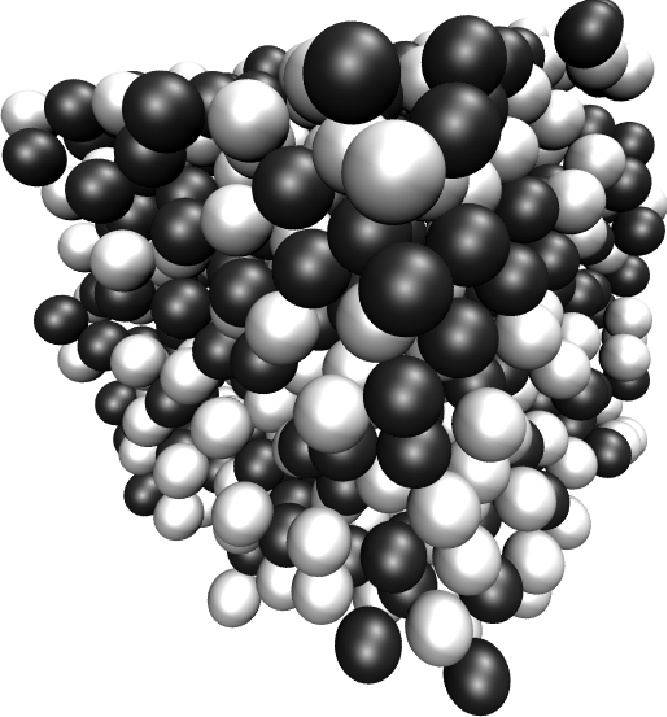
\includegraphics[width=0.4\textwidth]{figures/salt.png}
  \caption{VMD Snapshot of the salt system}
  \label{fig:snapshot}
\end{figure}

With these configurations, we can now investigate the system. As an example, we
will create a second script which calculates the averaged radial distribution
functions $g_{++}(r)$ and $g_{+-}(r)$. The radial distribution function for a
the current configuration can be obtained using the \verb|analyze| command:
\begin{tclcode}
set rdf [analyze rdf 0 1 0.9 [expr $box_l/2] 100]
set rlist ""
set rdflist ""
foreach value [lindex $rdf 1] {
  lappend rlist   [lindex $value 0]
  lappend rdflist [lindex $value 1] 
}
\end{tclcode}
The shown \verb|analyze rdf| command returns the distribution function of
particles of type 1 around particles of type 0 (i.~e.\ of opposite charges) for
radii between $0.9$ and half the box length, subdivided into $100$ bins.
Changing the first two parameters to either ``0 0'' or ``1 1'' allows to
determine the distribution for equal charges. The result is a list of $r$ and
$g(r)$ pairs, which the following foreach loop divides up onto two lists
\verb|rlist| and \verb|rdflist|.

To average over a set of configurations, we put the two last code snippets into
a loop like this:
\begin{tclcode}
set cnt 0
for {set i 0} {$i < 100} {incr i} { lappend avg_rdf 0}
foreach filename $argv {
  set f [open $filename "r"]
  while { [blockfile $f read auto] != "eof" } {}
  close $f
  set rdf [analyze rdf 0 1 0.9 [expr $box_l/2] 100]
  set rlist ""
  set rdflist ""
  foreach value [lindex $rdf 1] {
     lappend rlist   [lindex $value 0]
     lappend rdflist [lindex $value 1] }
  set avg_rdf [vecadd $avg_rdf $rdflist]
  incr cnt 
}
set avg_rdf [vecscale [expr 1.0/$cnt] $avg_rdf]
\end{tclcode}
Initially, the sum of all $g(r)$, which is stored in \verb|avg_rdf|, is set to
0.  Then the loops over all configurations given by \verb|argv|, calculates
$g(r)$ for each configuration and adds up all the $g(r)$ in \verb|avg_rdf|.
Finally, this sum is normalized by dividing by the number of
configurations. Note the ``1.0/\$cnt''; this is necessary, since ``1/\$cnt'' is
interpreted as an integer division, which results in 0 for $\text{cnt}>1$.
\verb|argv| is a predefined variable: it contains all the command line
parameters. Therefore this script should be called like
\begin{code}
Espresso \var{script} [\var{config}... ]
\end{code}

\begin{figure}[tb]
  \centering
  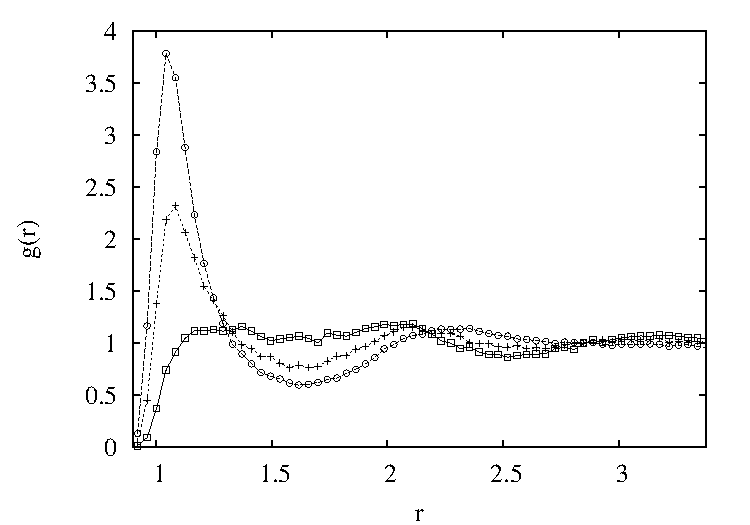
\includegraphics[width=0.7\textwidth]{figures/nacl-rdf.pdf}
  \caption{Radial distribution functions $g_{++}(r)$ between equal charges
    (rectangles) and $g_{+-}(r)$ for opposite charges (circles). The plus
    symbols denote $g(r)$ for an uncharged system.}
  \label{fig:rdf}
\end{figure}

The printing of the calculated radial distribution functions is simple. Add to the end of the
previous snippet the following lines:
\begin{tclcode}
set plot [open "rdf.data" "w"]
puts $plot "\# r rdf(r)"
foreach r $rlist rdf $avg_rdf { puts $plot "$r $rdf" }
close $plot
\end{tclcode}
This instructs the Tcl interpreter to write the \verb|avg_rdf| to the file \verb|rdf.data| in
gnuplot--compatible format. Fig.~\ref{fig:rdf} shows the resulting radial distribution functions,
averaged over 100 configurations. In addition, the distribution for a neutral
system is given, which can be obtained from our simulation script by simply
removing the command \verb|inter coulomb ...| and therefore not turning on P$^3$M.

The code example given before is still quite simple, and the reader is
encouraged to try to extend the example a little bit, e.~g. by using differently
sized particle, or changing the interactions. If something does not work, \es\
will give comprehensive error messages, which should make it easy to identify
mistakes. For real simulations, the simulation scripts can extend over thousands
of lines of code and contain automated adaption of parameters or online
analysis, up to automatic generation of data plots.  Parameters can be changed
arbitrarily during the simulation process, as needed for e.~g.\ simulated
annealing. The possibility to perform non--standard simulations without the need
of modifications to the simulation core was one of the main reasons why we
decided to use a script language for controlling the simulation core.

\section{\texttt{tutorial.tcl}}

In the directory \texttt{samples/} of the es{} sources, you will find
a well documented simulation script \texttt{tutorial.tcl}, which takes
you step by step through a slightly more complicated simulation of a
polyelectrolyte system. The basic structure of the script is however
the same as in the previous example and probably the same as the
structure of most \es{} simulation scripts.

Initially, some parameters and global variables are set, the
interactions are initialized, and particles are added. For this, the
script makes use of the \verb|polymer| command, which provides a
faster way to set up chain molecules.

The actual simulation falls apart again into two loops, the warmup
loop with increasing force capping, and the final simulation loop.
Note that the electrostatic interaction is only activated after
equilibrating the excluded volume interactions, which speeds up the
warmup phase. However, depending on the problem, this splitted warmup
may not be possible due to physical restrictions. \es{} cannot detect
these mistakes and it is your responsibility to find simulation
procedure suitable to your specific problem.

%%% Local Variables: 
%%% mode: latex
%%% TeX-master: "ug"
%%% End: 

\chapter{Compiling and installing \es}
\label{chap:install}
\index{Installation|textbf}

\begin{itemize}
\item Compiling \es{} is a necessary evil
\item Features can be compiled in or not
\item For maximal efficiency, compile in only the features that you
  use
\item \es{} can be obtained from the \es{} home page
  \footnote{\url{http://www.espresso.mpg.de}}.
\item If you are looking for the \es binary or the object files, read
  \vref{sec:builddir}
\item other than in most packages, \es will probably not be installed,
  or it will only be installed locally. Refer to \vref{sec:installdir}
  for details.
\end{itemize}

\section{Source and build directories}
\label{sec:builddir}
\index{build directory} \index{source directory}

Usually, when a program is compiled, the resulting binary files are
put into the same directory as the sources of the program. In \es, the
\emph{source directory} that contains all the source files is
completely separated from the \emph{build directory} where the files
created by the build process are put. As the source directory is not
modified during the compilation process, it is possible to compile more
than one binary versions of \es from a single set of source files.

The location of the build directory is determined when
\texttt{configure} is called.  Depending on whether it is called from
the source directory where it resides, or from some other directory,
the build system will act different.

When \texttt{configure} is called from another current working
directory than the source directory, this directory will become the
\emph{build directory}.  All files will be generated below the build
directory.  This way, you can make as many builds of \es as you like,
each build having different compiler flags and built-in features, and
for as many platforms as you want.  All further commands concerning
compiling and running \es{} have to be called from this directory,
instead of from the source directory.

When \texttt{configure} is called from the source directory where the
script resides, the \es build system has limited built-in capabilities
to handle different computer hardware.  A new subdirectory is created
in the source directory and \texttt{configure} is recursively called
from this directory, making the subdirectory the build directory.  The
directory is called \texttt{obj-}\textit{platform}\texttt{/}, where
\textit{platform} is an automatically determined descriptor of the CPU
type where the script was started, \eg
\mbox{\texttt{obj-Athlon\_64-pc-linux}}.  Note that this heuristic
will work in many cases, but it may not always work as intended.  When
you notice any problems, you can always call \texttt{configure} from
another directory.

In this case it is also possible to run the commands \texttt{make} and
\texttt{Espresso} directly in the source directory.  Furthermore, the
option \texttt{--enable-chooser} will be set in the recursive call of
\texttt{configure} that activates the automatic binary chooser (see
section \vref{sec:installdir}).

\paragraph{Example}
When the source directory is \texttt{\$srcdir} (\ie{} the files where
unpacked to this directory), then the build directory can be set to
\texttt{\$builddir} by calling the \texttt{configure}-script from
there:
\begin{code}
cd $builddir
$srcdir/configure
make
Espresso
\end{code}

\section{\texttt{myconfig.h}: Activating and deactivating features}
\label{sec:myconfig}

\index{features} \index{myconfig.h} \index{configuration header} \es
has a large number of features that can be compiled into the binary.
However, it is not recommended to actually compile in all possible
features, as this will negatively affect \es's performance.  Instead,
compile in only the features that are actually required.  For the
developers, it is also possible to turn on or off a number of
debugging messages.  The features and debug messages can be controlled
via a configuration header file that contains C-preprocessor
declarations. Appendix \vref{chap:features} lists and describes all
available features.  When no configuration header is provided by the
user, a default header will be used that turns on the default
features.  The file \texttt{myconfig-sample.h} in the source directory
contains a list of all possible features that can be copied into your
own configuration file.

When you distinguish between the build and the source directory (see
\vref{sec:builddir}), the configuration header can be put in either of
these. Note, however, that when a configuration header is found in
both directories, the one in the build directory will be used.  For an
example how this can be employed, see section \ref{sec:builddir}.

By default, the configuration header is called \texttt{myconfig.h}.
The name of the configuration header can be changed either when the
\texttt{configure}-script is called with the option
\mbox{\texttt{--with-myconfig}} (see section \vref{sec:configure}), or
when \texttt{make} is called with the setting
\mbox{\texttt{myconfig=}\textit{myconfig\_header}} (see section
\vref{sec:make}).

The configuration header can be used to compile different binary
versions of \es with a different set of features from the same source
directory.  Suppose that you have a source directory \texttt{\$srcdir}
and two build directories \texttt{\$builddir1} and
\texttt{\$builddir2} that contain different configuration headers:

\begin{itemize}
\item \texttt{\$builddir1/myconfig.h}:
\begin{code}
#define ELECTROSTATICS
#define LENNARD-JONES
\end{code}

\item \texttt{\$builddir2/myconfig.h}:
\begin{code}
#define LJCOS
\end{code}
\end{itemize}

\noindent Then you can simply compile two different versions of \es via
\begin{code}
cd $builddir1
$srcdir/configure
make

cd $builddir2
$srcdir/configure
make
\end{code}


\section{Running \texttt{configure}}
\label{sec:configure}

% Description of basic options: --prefix, --exec-prefix, CPPFLAGS,
% CFLAGS, LDFLAGS

\index{configure} The shell script \texttt{configure} collects all the
information required by the compilation process. It will determine how
to use and where to find the different libraries and tools required by
the compilation process, and it will test what compiler flags are to
be used.  The script will find out most of these things automatically.
If something is missing, it will complain and give hints how to solve
the problem.  The generic syntax of calling the \texttt{configure}
script is:
\begin{code}
configure [\var{options} ...] [\var{variable}=\var{value} ...]
\end{code}

\noindent Note that in the \es build system, the files generated by
the configuration and compilation process are not placed next to the
source files, but into a separate \emph{build directory} instead.
Refer to section \vref{sec:builddir} for details.

\index{configure options} The behaviour of \texttt{configure} can be
controlled by the means of command line options. In the following,
only those command line options that are specific to \es will be
explained.  For a complete list of options and explanations thereof,
call
\begin{code}
configure --help
\end{code}

\subsection{Options}

\begin{description}
\item [\texttt{--enable-chooser}] This option will enable the
  automatic binary chooser mechanism for \es (see section
  \vref{sec:installdir}).  This option will be automatically enabled,
  when the \texttt{configure} script is called from the source
  directory, otherwise it will be disabled. It is not recommended to
  set the option manually.
\item[\texttt{--enable-debug}] This option will enable compiler flags
  required for debugging the \es binary and is disabled by default.
\item[\texttt{--enable-profiling}] This option will enable compiler
  flags required for profiling the \es binary and is disabled by
  default.
\item[\texttt{--disable-processor-optimization}] This option will
  control whether \texttt{configure} will check for several
  optimization flags to be used by the compiler. This option is
  enabled by default.
\item[\texttt{--disable-xlc-qipa}] This option is only useful when the
  IBM C-compiler \texttt{xlc} is used and will control whether or not
  the compiler flag \texttt{-qipa} is used.  If you come upon problems
  when using the \es binary on IBM machines, try using
  \texttt{--disable-xlc-ipa}. The option is enabled by default.
\item[\texttt{--with-myconfig=MYCONFIG\_HEADER}] This option sets the
  name of the local configuration header (see \vref{sec:myconfig}). It
  defaults to ``\texttt{myconfig.h}''.
\item[\texttt{--with-mpi=MPI}/ \texttt{--without-mpi}] Sets the MPI
  implementation that should be used, or disables MPI. By default,
  \texttt{configure} will test automatically what MPI implementation
  is available. The following implementations are known:
  \begin{description}
  \item[\texttt{fake}, \texttt{no}] This will disable MPI
    completely. Equivalent to \mbox{\texttt{--without-mpi}}.
  \item[\texttt{lam}] Use the LAM/MPI environment
    (\url{http://www.lam-mpi.org/}).
  \item[\texttt{mpich}] Use the MPICH environment
    (\url{http://www-unix.mcs.anl.gov/mpi/mpich/}).
  \item[\texttt{poe}] Use the POE environment (IBM).
  \item[\texttt{dmpi}] Use the DMPI environment (Tru64).
  \item[\texttt{generic}] Use a generic MPI implementation. This will
    try to find an MPI compiler and an MPI runtime environment.
  \end{description}
\item[\texttt{--with-efence} / \texttt{--without-efence}] Whether or
  not to use the ``electric fence'' memory debugging library
  (\url{http://freshmeat.net/projects/efence/}). Efence is not used by
  default.
\item[\texttt{--with-tcl=TCL}] By default, \texttt{configure} will
  automatically determine which version of Tcl is used.  If the wrong
  version is chosen automatically, you can specify the name of the
  library with this option, \eg{} \texttt{tcl8.4}.
\item[\texttt{--with-tk=TK} / \texttt{--without-tk}] By default, the
  GUI toolkit Tk is not used by \es. This option can be used to
  activate Tk and to specify which Tk version to use, \eg{}
  \texttt{tk8.4}. If you only specify \texttt{--with-tk} and do not
  give a version number, \texttt{configure} will try to automatically
  deduce the right version.
\item[\texttt{--with-fftw=VERSION} / \texttt{--without-fftw}] This can
  be used to specify whether the FFTW library is to be used, and which
  version.  By default, version 3 will be used if it is found,
  otherwise version 2 is used.  Note that quite a number of central
  features of \es require FFTW.
\end{description}

\section{\texttt{make}: Compiling,  testing and installing \es}
\label{sec:make}

The command \texttt{make} is mainly used to compile the \es{} source
code, but it can do a number of other things. The generic syntax of
the \texttt{make} command is:
\begin{code}
make [\var{target}...] [\var{variable}=\var{value}]
\end{code}
When no target is given, the target \texttt{all} is used. The
following targets are available:
\begin{description}
\item[\texttt{all}] Compiles the complete \es source code. The
  variable \lit{myconf} can be used to specify the name of the
  configuration header to be used.
\item[\texttt{check}] Runs the testsuite. By default, all available
  tests will be run on 1, 2, 3, 4, 6, or 8 processors. Which tests are
  run can be controlled by means of the variable \texttt{tests}, which
  processor numbers are to be used can be controlled via the variable
  \texttt{processors}. Note that depending on your MPI installation,
  MPI jobs can only be run in the queueing system, so that \es{} will
  not run from the command line. In that case, you may not be able to
  run the testsuite, or you have to directly submit the testsuite script
  \verb!testsuite/test.sh! to the queueing system.\\
  \textbf{Example:} \verb!make check tests="madelung.tcl" processors="1 2"!\\
  will run the test \texttt{madlung.tcl} on one and two processors.
\item[\texttt{clean}] Deletes all files that were created during the
  compilation.
\item[\texttt{mostlyclean}] Deletes most files that were created
  during the compilation. Will keep for example the built doxygen
  documentation and the \es{} binary.
\item[\texttt{dist}] Creates a \texttt{.tar.gz}-file of the \es{}
  sources.  This will include all source files as they currently are
  in the source directory, \ie{} it will include local changes.  This
  is useful to give your version of \es{} to other people.
  The variable \texttt{extra} can be used to specify additional
  files and directories that are to be included in the archive
  file. \\
  \textbf{Example:} \verb!make dist extra="myconfig.h internal"!\\
  will create the archive file and include the file
  \texttt{myconfig.h} and the directory \texttt{internal} with all
  files and subdirectories.
\item[\texttt{install}] Install \es. The variables \texttt{prefix} and
  \texttt{exec-prefix} can be used to specify the installation
  directories, otherwise the defaults defined by the
  \texttt{configure} script are used. \texttt{prefix} sets the prefix
  where all \es files are to be installed, \texttt{exec-prefix} sets
  the prefix where the executable files are to be installed and is
  required only when there is an architecture-specific directory (\eg
  \texttt{/usr/local/bin64/}).  For the actual locations where the
  different files are installed, refer to section
  \vref{sec:installdir}.\\
  \textbf{Example:} \verb!make install prefix=/usr/local!\\
  will install all files below \texttt{/usr/local}.
\item[\texttt{uninstall}] Uninstalls \es{}, \ie{} removes all files
  that were installed during \texttt{make install}. The variables are
  identical to the variables of the \texttt{install}-target.
\end{description}

\subsection{Installation directories}
\label{sec:installdir}

\index{installation directory} Other than most software, \es is not
necessarily installed into the system, but can also be used directly
from the build directory.  The rest of this section is only
interesting if you plan to install \es.

Normally, the \es-binary \texttt{Espresso-bin} is installed in the
directory \texttt{\$prefix/libexec/} and a the wrapper script
\texttt{Espresso} in the directory \texttt{\$prefix/bin/} that handles
the MPI invocation.

When the \texttt{configure}-script is called from the source directory
or when the option \texttt{--enable-chooser} is given, an automatic
binary chooser is installed in the directory \texttt{\$prefix/bin/}
and the \es-binary and the MPI wrapper script are installed in an
architecture-specific subdirectory
\mbox{\texttt{\$exec-prefix/lib/espresso/obj-}\textit{platform}\texttt{/}}.
When called, the binary chooser will automatically call the MPI
wrapper script from the right subdirectory.

\section{Running \es}
\label{sec:run}

When \es is found in your path, it can be run via
\begin{code}
Espresso [\var{tcl\_script} [\var{N\_processors} [\var{args}]]]
\end{code}

\index{interactive mode} When \es{} is called without any arguments,
it is started in the interactive mode, where new commands can be
entered on the command line. When the name of a \textit{tcl\_script}
is given, the script is executed. \textit{N\_processors} is the number
of processors that are to be used. Any further arguments are passed to
the script. Note that depending on your MPI installation, MPI jobs can
only be run in the queueing system, so that \es will not run from
the command line.

% A number of wrapper scripts are used in running \es{}:
% \begin{itemize}
% \item The script \texttt{Espresso} in the source and build directory
%   will try to run the compiled version of \es. If it is called from
%   the source directory, it assumes that \es{} was also configured in
%   the source directory and will try to recursively start the script in
%   the corresponding \texttt{obj-PLATFORM} build directory. If it is
%   called in the build directory, it will start the \es-binary with the
%   right MPI implementation.
% \item The chooser script \texttt{Espresso} 
%   \begin{itemize}
%   \item installed when \verb!--enable-chooser! was given
%   \item installed to bindir
%   \item tries to run the correct version of the MPI-wrapper
%     \texttt{Espresso}
%   \end{itemize}
% \item The MPI-wrapper \texttt{Espresso}
%   \begin{itemize}
%   \item installed next to \es{} binary
%   \item starts the binary with the right MPI implementation
%   \end{itemize}
% \item The \es{} binary \texttt{Espresso-bin} can also be started
%   directly, however, it requires that the environment variable
%   \verb!ESPRESSO_SCRIPTS! is set to the directory where the scripts
%   are installed (usually \verb!$(prefix)/lib/espresso/scripts! or
%   \verb!$(prefix)/share/espresso/scripts!).
% \end{itemize}


%%% Local Variables: 
%%% mode: latex
%%% TeX-master: "ug"
%%% End: 


\chapter{Setting up particles}
\label{chap:part}

\section{\texttt{part}: Creating single particles}
\newescommand{part}

\subsection{Defining particle properties}

\begin{essyntax}
  part
  \var{particle_number}
  \opt{pos \var{x} \var{y} \var{z}}
  \opt{type \var{particle_type_number}}
  \opt{v \var{vx} \var{vy} \var{vz}}
  \opt{f \var{fx} \var{fy} \var{fz}}
  \opt{bond \var{bond_type_number} \var{partner} \dots}
  \require{1}{\opt{q \var{charge}}}
  \require{2}{\opt{quat \var{q1} \var{q2} \var{q3} \var{q4}}}
  \require{2}{\opt{omega \var{x_value} \var{y_value} \var{z_value}}}
  \require{2}{\opt{torque \var{x_value} \var{y_value} \var{z_value}}}\\
  \require{3}{\opt{\opt{un}fix \var{x} \var{y} \var{z}}}
  \require{3}{\opt{ext_force \var{x_value} \var{y_value} \var{z_value}}}
  \require{4}{\opt{exclude \var{exclusion_partner}\dots}}
  \require{4}{\opt{exclude delete \var{exclusion_partner}\dots}}
  \require{5}{\opt{mass \var{mass}}}
  \require{6}{\opt{dipm \var{moment}}}
  \require{6}{\opt{dip \var{dx} \var{dy} \var{dz}}}
  \begin{features}
    \required[1]{ELECTROSTATICS} 
    \required[2]{ROTATION}
    \required[3]{EXTERNAL_FORCES}
    \required[4]{EXCLUSION}
    \required[5]{MASS}
    \required[6]{DIPOLES}
  \end{features}
\end{essyntax}

This command modifies particle data, namely position, type (monomer,
ion, \dots), charge, velocity, force and bonds. Multiple properties can
be changed at once. If you add a new particle the position has to be
set first because of the spatial decomposition.

\begin{arguments}
\item[\var{particle_number}]
\item[\opt{pos \var{x} \var{y} \var{z}}] Sets the position of this
  particle to $(x,y,z)$.
\item[\opt{type \var{particle_type_number}}] Restrictions:
  $\var{particle_type_number} \geq 0$.\\ The
  \var{particle_type_number} is used in the \keyword{inter} command
  (see section \vref{tcl:inter}) to define the parameters of the non
  bonded interactions between different kinds of particles.
\item[\opt{v \var{vx} \var{vy} \var{vz}}] Sets the velocity of
this particle to $(vx,vy,vz)$. The velocity remains variable and will be changed
during integration.
\item[\opt{f \var{fx} \var{fy} \var{fz}}] Set the force acting on this particle
to $(fx,fy,fz)$. The force remains variable and will be changed during integration.
\item[\opt{bond \var{bond_type_number} \var{partner}+}]
  Restrictions: \var{bond_type_number} $\geq 0$; \var{partner} must
  be an existing particle.  The \var{bond_type_number} is used for
  the inter command to define bonded interactions.
\item[bond delete] Will delete all bonds attached to this particle.
\item[\opt{q \var{charge}}] Sets the charge of this praticle to $q$.
\item[\opt{quat \var{q1} \var{q2} \var{q3} \var{q4}}] \todo{Docs required (JC?).} 
  \item[\opt{omega \var{x_value} \var{y_value} \var{z_value}}] \todo{Docs
  required (JC?).} 
  \item[\opt{torque \var{x_value} \var{y_value} \var{z_value}}] \todo{Docs
  required (JC?).}
\item[\opt{fix \var{x} \var{y} \var{z}}] Fixes the particle in space.
  By supplying a set of 3 integers as arguments it is possible to fix
  motion in \var{x}, \var{y}, or \var{z} coordinates independently. For
  example \var{fix 0 0 1} will fix motion only in z. Note that
  \var{fix} without arguments is equivalent to \var{fix 1 1 1}.
\item[\opt{ext_force \var{x_value} \var{y_value} \var{z_value}}]
  An additional external force is applied to the particle.
\item[\opt{unfix}] Release any external influence from the particle.
\item[\opt{exclude \var{exclusion_partner}+}] Restrictions:
  \var{exclusion_partner} must be an existing particle.  Between the
  current particle an the exclusion partner(s), no nonbonded
  interactions are calculated. Note that unlike bonds, exclusions are
  stored with both partners.  Therefore this command adds the defined
  exclusions to both partners.
\item[\opt{exclude delete \var{exclusion_partner}+}] Searches for the
  given exclusion and deletes it. Again deletes the exclusion with
  both partners.
  \item[\opt{mass \var{mass}}] Sets the mass of this particle to $mass$. If not
  set, all particles have a mass of 1 in reduced units.
  \item[\opt{dipm \var{moment}}] Sets the dipol moment of this particle to $moment$.
  \item[\opt{dip \var{dx} \var{dy} \var{dz}}] Sets the orientation of the
  dipol axis to $(dx,dy,dz)$.
 
  \end{arguments}
\subsection{Getting particle properties}

\begin{essyntax}
  \variant{1}
  part \var{particle_number} print
  \optlong{\alt{id \asep pos \asep type \asep folded_position \asep type \asep
      q \asep v \asep f \asep fix \asep ext_force \asep bond \asep
      \mbox{connections \opt{\var{range}}}}}\dots
  \variant{2} part
\end{essyntax}

Variant \variant{1} will return a list of the specified properties of
particle \var{particle_number}, or all properties, if no keyword is
specified.  Variant \variant{2} will return a list of all properties
of all particles.

\minisec{Example}
\begin{code}
part 40 print id pos q bonds
\end{code}
will return a list like
\begin{tclcode}
40 8.849 1.8172 1.4677 1.0 {}
\end{tclcode}
This routine is primarily intended for effective use in Tcl scripts.

When the keyword \keyword{connection} is specified, it returns the
connectivity of the particle up to \var{range} (defaults to 1). For
particle 5 in a linear chain the result up to \var{range} = 3 would
look like:
\begin{tclcode}
{ { 4 } { 6 } } { { 4 3 } { 6 7 } } { {4 3 2 } { 6 7 8 } } 
\end{tclcode}
The function is useful when you want to create bonded interactions to
all other particles a certain particle is connected to. Note that this
output can not be used as input to the part command. Check results if
you use them in ring structures.

If none of the options is specified, it returns all properties of the
particle, if it exists, in the form
\begin{tclcode}
  0 pos 2.1 6.4 3.1 type 0 q -1.0 v 0.0 0.0 0.0 f 0.0 0.0 0.0
  bonds { {0 480} {0 368} ... } 
\end{tclcode}
which may be used as an input to this function later on. The first
integer is the particle number.

Variant \variant{2} returns the properties of all stored particles in
a tcl-list with the same format as specified above:
\begin{tclcode}
{0 pos 2.1 6.4 3.1 type 0 q -1.0 v 0.0 0.0 0.0 f 0.0 0.0 0.0
 bonds{{0 480}{0 368}...}} 
{1 pos 1.0 2.0 3.0 type 0 q 1.0 v 0.0 0.0 0.0 f 0.0 0.0 0.0
 bonds{{0 340}{0 83}...}} 
{2...{{...}...}}
{3...{{...}...}}
...
\end{tclcode}

\subsection{Deleting  particles}
\label{tcl:part:delete}

\begin{essyntax}
  \variant{1} part \var{particle_number} delete
  \variant{2} part deleteall
\end{essyntax}

In variant \variant{1}, the particle \var{particle_number} is deleted
and all bonds referencing it.  Variant \variant{2} will delete all
particles currently present in the simulation. Variant \variant{3}
will delete all currently defined exclusions.

\subsection{Exclusions}

\begin{essyntax}
  \variant{1} part auto_exclusions \opt{\var{range}}
  \variant{2} part delete_exclusions
\end{essyntax}

Variant \variant{1} will create exclusions for all particles pairs
connected by not more than \var{range} bonds (\var{range} defaults to
2). This is typically used in atomistic simulations, where nearest and
next nearest neighbour interactions along the chain have to be omitted
since they are included in the bonding potentials. For example, if the
system contains particles $0$ \dots $100$, where particle $n$ is
bonded to particle $n-1$ for $1 \leq n \leq 100$, then it will result
in the exclusions:
\begin{itemize}
  \item particle 1 does not interact with particles 2 and 3
  \item particle 2 does not interact with particles 1, 3 and 4
  \item particle 3 does not interact with particles 1, 2, 4 and 5
  \item ...
\end{itemize}

Variant \variant{2} deletes all exclusions currently present in the
system.

\section{Creating groups of particle}

\subsection{\texttt{polymer}: Setting up polymer chains}

\newescommand{polymer}
\begin{essyntax}
  polymer 
  \var{num_polymers} \var{monomers_per_chain}
  \var{bond_length}\\
  \opt{start \var{part_id}} 
  \opt{pos \var{x} \var{y} \var{z}}
  \opt{mode \alt{RW \asep SAW \asep PSAW} 
    \opt{\var{shield} \opt{\var{max_try}}}} 
  \require{1}{\opt{charge \var{val_charged_monomer}}} 
  \require{1}{\opt{distance \var{dist_charged_monomer}}}
  \opt{types \var{type_neutral_monomer}
    \opt{\var{type_charged_monomer}}} 
  \opt{bond \var{type_bond}} 
  \opt{angle \var{phi} \opt{\var{theta} \opt{\var{x} \var{y}
        \var{z}}}}
  \require{2}{\opt{constraints}}
  \begin{features}
    \required[1]{ELECTROSTATICS}
    \required[2]{CONSTRAINTS}
  \end{features}
\end{essyntax}

This command will create \var{num_polymers} polymer or
polyelectrolyte chains with \var{monomers_per_chain} monomers per
chain. The length of the bond between two adjacent monomers will be
set up to be \var{bond_length}.

\begin{arguments}
\item[\var{num_polymers}] Sets the number of polymer chains.
\item[\var{monomers_per_chain}] Sets the number of monomers per
  chain.
\item[\var{bond_length}] Sets the initial distance between two adjacent
  monomers. The distance during the course of the simulation depends on the
  applied potentials. For fixed box length please refer to the SHAKE algorithm.
  \todo{Link to rattle/shake.}
\item[\opt{start \var{part_id}}] Sets the particle number of the
  start monomer to be used with the \keyword{part} command. This
  defaults to 0.

\item[\opt{pos \var{x} \var{y} \var{z}}] Sets the position of the
  first monomer in the chain to \var{x}, \var{y}, \var{z} (defaults to
  a randomly chosen value)
  
\item[\opt{mode \alt{RW  \asep  PSAW  \asep  SAW} \opt{\var{shield}
      \opt{\var{max_try}}}}]
  Selects the setup mode:
  \begin{description}
  \item[\keyword{RW} (Random walk)] The monomers are
    randomly placed by a random walk with a steps size of
    \var{bond_length}.
  \item[\keyword{PSAW} (Pruned self-avoiding walk)] The position of a
    monomer is randomly chosen in a distance of \var{bond_length} to
    the previous monomer. If the position is closer to another
    particle than \var{shield}, the attempt is repeated up to
    \var{try_max} times. Note, that this is not a real self-avoiding
    random walk, as the particle distribution is not the same. If you
    want a real self-avoiding walk, use the \keyword{SAW} mode.
    However, \keyword{PSAW} is several orders of magnitude faster than
    \keyword{SAW}, especially for long chains.
  \item[\keyword{SAW} (Self-avoiding random walk)] The positions of
    the monomers are chosen as in the plain random walk. However, if
    this results in a chain that has a monomer that is closer to
    another particle than \var{shield}, a new attempt of setting up
    the whole chain is done, up to \var{max_try} times.
  \end{description}
  The default for the mode is \keyword{RW}, the default for the
  \var{shield} is $1.0$, and the default for \var{max_try} is
  $30000$, which is usually enough for \keyword{PSAW}. Depending on
  the length of the chain, for the \keyword{SAW} mode, \var{max_try}
  has to be increased by several orders of magnitude.
\item[\opt{charge \var{val_charged_monomer}}] Sets the valency of
  the charged monomers.  If the valency of the charged polymers
  \var{val_charged_monomer} is smaller than $10^{-10}$, the charge
  is assumed to be zero, and the types are set to
  \var{type_charged_monomer} = \var{type_neutral_monomer}. If charge is not set,
  it defaults to 0.0.

\item[\opt{distance \var{dist_charged_monomer}}] Sets the stride
  between the indices of two charged monomers. This defaults defaults
  to 1, meaning that all monomers in the chain are charged.
  
\item[\opt{types \var{type_neutral_monomer}
    \var{type_charged_monomer}}] Sets the type numbers of the
  neutral and charged monomer types to be used with the \keyword{part}
  command. If \var{type_neutral_monomer} is defined,
  \var{type_charged_monomer} defaults to 1. If the option is
  omitted, both monomer types default to 0.
  
\item[\opt{bond \var{type_bond}}] Sets the type number of the bonded
  interaction to be set between the monomers. This defaults to 0. Any bonded
  interaction, no matter how many bonding-partners needed, is stored with the
  second particle in this bond. \todo{Link to
  bonded interactions}
  
\item[\opt{angle \var{phi} [\var{theta} [\var{x} \var{y} \var{z}]]}]
  Allows for setting up helices or planar polymers: \var{phi} sets
  the angle $\phi$ and \var{theta} sets the angle $\theta$ between
  adjacent bonds. \var{x}, \var{y} and \var{z} set the position of the
  second monomer of the first chain.
  \item[\opt{constraints}] If this option is specified, the particle setup-up
  tries to obey previously defined constraints (see Section \vref{sec:constraint}).
\end{arguments}

\subsection{\texttt{counterions}: Set up counterions}
\newescommand{counterions}
\begin{essyntax}
  counterions
  \var{N_CI} 
  \opt{start \var{part_id}} 
  \opt{mode \alt{SAW \asep RW} \opt{\var{shield} \opt{\var{max_try} }}} 
  \require{1}{\opt{charge \var{val_CI}}}
  \opt{type \var{type_CI}}
  \begin{features}
    \required[1]{ELECTROSTATICS}
  \end{features}
\end{essyntax}
This command will create \var{N_CI} counterions in the simulation box.
\begin{arguments}
  \item[\var{N_CI}] Sets the number of counterions to setup.
  \item[\opt{start \var{part_id}}] Sets the particle id of the first counterion.
  It defaults to the current number of particles, \ie counterions are placed
  after all previously defined particles.
  \item[\opt{mode \alt{SAW \asep RW} \opt{\var{shield} \opt{\var{max_try} }}}]
  Specifies the setup method to place the counterions. It defaults to
  \texttt{SAW}. See the \texttt{polymer} command for a detailed description.
  \item[\opt{charge \var{val_CI}}] Specifies the charge of the counterions. If not
  set, it defaults to -1.0.
  \item[\opt{type \var{type_CI}}] Specifies the particle type of the counterions. It
  defaults to 2.
\end{arguments}

\smallskip
\subsection{\texttt{salt}: Set up salt ions}
\newescommand{salt}
\begin{essyntax}
  salt 
  \var{N_pS} \var{N_nS} 
  \opt{start \var{part_id}} 
  \opt{mode \alt{SAW \asep RW} \opt{\var{shield} \opt{\var{max_try}}}}
  \require{1}{\opt{charges \var{val_pS} \opt{\var{val_nS}}}} 
  \opt{types \var{type_pS} \opt{\var{type_nS}}}
  \opt{rad \var{radius}}
  \begin{features}
    \required[1]{ELECTROSTATICS}
  \end{features}
\end{essyntax}

Create \var{N_pS} positively and \var{N_nS} negatively charged salt
ions of charge \var{val_pS} and \var{val_nS} within the simulation
box.
\begin{arguments}
  \item[\var{N_pS}] Sets the number of positively charged salt ions.
  \item[\var{N_nS}] Sets the number of negatively charged salt ions.
  \item[\opt{start \var{part_id}}] Sets the particle id of the first
  (positively charged) salt ion. It defaults to the current number of particles.
  \item[\opt{mode \alt{SAW \asep RW} \opt{\var{shield} \opt{\var{max_try} }}}]
  Specifies the setup method to place the counterions. It defaults to 
  \texttt{SAW}. See the \texttt{polymer} command for a detailed description.
  \item[\opt{charge \var{val_pS} \opt{\var{val_nS}}}] Sets the charge of the
  positive salt ions to \var{val_pS} and the one of the negatively charged salt
  ions to \var{val_nS}. If not set, the values default to 1.0 and -1.0.
  \item[\opt{type \var{type_pS} \opt{\var{type_nS}}}] Specifies the particle type of the
  salt ions. It defaults to 3 for positive ions and 4 for negative ions.
  \item[\opt{rad \var{radius}}] When working within the cell model, the salt
  ions are only placed in a sphere with radius \var{radius} around the origin. 
\end{arguments}


\subsection{\texttt{diamond}: Setting up diamond polymer networks}
\newescommand{diamond}
\begin{essyntax}
  diamond 
  \var{a} \var{bond_length} \var{MPC} 
  \opt{counterions \var{N_CI}} 
  \require{1}{\opt{charges \var{val_nodes} \var{val_cM} \var{val_CI}}}
  \require{1}{\opt{distance \var{cM_dist}}}
  \opt{nonet}
  \begin{features}
    \required[1]{ELECTROSTATICS}
  \end{features}
\end{essyntax}

Creates a diamond-shaped polymer network with 8 tetra-functional nodes
connected by $2*8$ polymer chains of length \var{MPC} in a unit cell of length
\var{a}. For inter-particle bonds interaction 0 is taken which must be a
two-particle bond. \todo{A picture would be helpful.}

\begin{arguments}
  \item[\var{a}] Determines the size of the of the unit cell.
  \item[\var{bond_length}] Specifies the bond length of the polymer chains
  connecting the 8 tetra-functional nodes.
  \item[\var{MPC}] Sets the number of chain monomers between the funtional
  nodes.
  \item[\opt{counterions \var{N_CI}}] Adds \var{N_CI} counterions to the system.
  
  \item[\opt{charges \var{val_nodes} \var{val_cM} \var{val_CI}}] Sets the
  charges of the nodes to \var{val_nodes}, the charge of the connecting monomers
  to \var{val_cM}, and the charge of the counterions to \var{val_CI}.
  \item[\opt{distance \var{cM_dist}}] Specifies the distance between charged
  monomers along the interconnecting chains. If $\var{cM_dist} > 1$ the remaining
  chain monomers are uncharged.
  \item[\opt{nonet}] \todo{Define what \var{nonet} does.}
\end{arguments}


\subsection{\texttt{icosaeder}: Setting up an icosaeder}
\newescommand{icosaeder}
\begin{essyntax}
  icosaeder 
  \var{a} \var{MPC} 
  \opt{counterions \var{N_CI}} 
  \require{1}{\opt{charges \var{val_cM} \var{val_CI}}}
  \require{1}{\opt{distance \var{cM_dist}}}
  \begin{features}
    \required[1]{ELECTROSTATICS}
  \end{features}
\end{essyntax}

Creates a modified icosaeder to model a fulleren (or soccer ball). The edges are
modeled by polymer chains connected at the corners of the icosaeder. For 
inter-particle bonds interaction 0 is taken which must be a two-particle bond.
\todo{A picture would be helpful}

\begin{arguments}
  \item[\var{a}] Defines the size of the icosaeder.
  \item[\var{MPC}] Specifies the number of chain monomers along one edge.
  \item[\opt{counterions \var{N_CI}}] Specifies the number of counterions to be
  placed into the system.
  \item[\opt{charges \var{val_cM} \var{val_CI}}] Set the charges of the monomers
  to \var{val_cM} and the charges of the counterions to \var{val_CI}.
  \item[\opt{distance \var{cM_dist}}] Specifies the distance between two charged
  monomer along the edge. If $\var{cM_dist} > 1$ the remaining monomers are uncharged.
\end{arguments}

\subsection{\texttt{crosslink}: Cross-linking polymers}
\newescommand{crosslink}
\begin{essyntax}
  crosslink 
  \var{N_P} \var{MPC} 
  \opt{start \var{part_id}} 
  \opt{catch \var{r_catch}}
  \opt{distLink \var{link_dist}} 
  \opt{distChain \var{chain_dist}} 
  \opt{FENE \var{type_FENE}} 
  \opt{trials \var{max_try}} 
\end{essyntax}

Attempts to end-crosslink the current configuration of \var{N_P}
equally long polymers with \var{MPC} monomers each, returning how many
ends are successfully connected. 

\begin{arguments}
  \item[\var{N_P}] The number of polymers in the current configuration to be
  linked. 
  \item[\var{MPC}] The number of monomers per chain to be linked.
  \item[\opt{start \var{part_id}}] \var{part_id} specifies the first monomer of
  the chains to be linked. It has to be specified if the polymers do not start
  at id 0.
  \item[\opt{catch \var{r_catch}}] Set the radius around each monomer which is
  searched for possible new monomers to connect to. \var{r_catch} defaults to
  1.9.
  \item[\opt{distLink \var{link_dist}}] The minimal distance of two
  interconnecting links. It defaults to 2.
  \item[\opt{distChain \var{chain_dist}}] The minimal distance for an
  interconnection along the same chain. It defaults to 0. If set to \var{MPC},
  no interchain connections are created.
  \item[\opt{FENE \var{type_FENE}}] Sets the bond type for the connections to \var{type_FENE}.
  \item[\opt{trials \var{max_try}}] If not specified, \var{max_try} defaults to 30000.
\end{arguments}

\section{\texttt{constraint}: Setting up constraints}\label{sec:constraint}
\newescommand{constraint}

\begin{essyntax}
  \variant{1} 
  constraint wall normal \var{n_x} \var{n_y} \var{n_z} 
  dist \var{d} type \var{id}
  
  \variant{2}
  constraint sphere center \var{c_x} \var{c_y} \var{c_z} 
  radius \var{rad} direction \var{direction} type \var{id} 
  
  \variant{3}
  constraint cylinder center \var{c_x} \var{c_y} \var{c_z} 
  axis \var{n_x} \var{n_y} \var{n_z} 
  radius \var{rad} length \var{length} 
  direction \var{direction} 
  type \var{id} 
  
  \variant{4}
  constraint maze nsphere \var{n} 
  dim \var{d} sphrad \var{r_s} cylrad \var{r_c}
  type \var{id}
  
  \variant{5}  
  constraint pore center \var{c_x} \var{c_y} \var{c_z} 
  axis \var{n_x} \var{n_y} \var{n_z} 
  radius \var{rad} length \var{length} 
  type \var{id} 
  
  \require{1}{%
    \variant{6}
    constraint rod center \var{c_x} \var{c_y} 
    lambda \var{lambda}
  } 
  
  \require{1}{%
    \variant{7}
    constraint plate height \var{h}
    sigma \var{sigma} 
  }
  
  \require{2,3}{%
    \variant{8}
    constraint ext_magn_field \var{f_x} \var{f_y} \var{f_z} 
  }

  \begin{features}
    \required{CONSTRAINTS}
    \required[1]{ELECTROSTATICS}
    \required[2]{ROTATION}
    \required[3]{DIPOLES}
  \end{features}
\end{essyntax}

\todo{Does this command really work only with the LJ potential, or
  with any short-ranged potential?}
The \codebox{constraint} command offers a variety of surfaces that can be
defined to interact with desired particles. Variants \variant{1} to \variant{5}
create interactions via a
Lennard-Jones potential. \[4 \epsilon \left(\left(\frac{\sigma}{r}\right)^{12} -
  \left(\frac{\sigma}{r}\right)^6 + shift\right)\] with r being the
distance of the center of the particle to the surface. The constraints are identified like a particle via its
type for the lennard-jones force calculation. 
After a type is defined for each constraint one has
to define
the interaction of all different particle types with the constraint using
the \codebox{inter} command.

Variants \variant{6} and \variant{7} create interactions based on electrostatic
interactions. The corresponding force acts in direction of the normal vector of the
surface and applies to all charged particles.

Variant \variant{8} does not define a surface but is based on magnetic
dipolar interaction with an external magnetic field. It applies to all particles
with a dipol moment.

\textbf{Note that constraints are not saved to checkpoints and that they have to
be reset upon restarting a simulation.}

The resulting surface in variant \variant{1} is a plane defined by the
normal vector \var{n_x} \var{n_y} \var{n_z} and the distance
\var{d} from the origin. The force acts in direction of the normal. 

The resulting surface in variant
\variant{2} is a sphere with center \var{c_x} \var{c_y} \var{c_z} and radius
\var{rad}. The \var{direction} determines the force direction, -1 or
\opt{inside} for inward and +1 or \opt{outside} for outward. 

The resulting surface
in variant \variant{3} is a cylinder with center \var{c_x} \var{c_y}
\var{c_z} and radius \var{rad}. The \var{length} parameter is \textbf{half} 
of the cylinder length. The \var{axis} is a
vector along the cylinder axis, which is normalized in the program.
The \var{direction} is defined the same way as for the spherical
constraint. 

The resulting surface in variant \variant{4} is \var{n}
spheres of radius \var{r_s} along each dimension, connected by
cylinders of radius \var{r_c}. The spheres have simple cubic
symmetry. The spheres are distributed evenly by dividing the
\var{box_l} by \var{n}.  Dimension of the maze can be controlled by
\var{d}: 0 for one dimensional, 1 for two dimensional and 2 for three
dimensional maze.

Variant \variant{5} sets up a cylindrical pore similar to variant \variant{3} 
with a center
\var{c_x}
\var{c_y}
\var{c_z} and radius \var{rad}. The \var{length} parameter is \textbf{half} 
of the cylinder length. The \var{axis} is a
vector along the cylinder axis, which is normalized in the program.
\todo{Is this command obsolete? Cylinder?}

Variant \variant{6} specifies an electrostatic interaction between the charged
particles in the system to an infinitely long rod with a
line charge of \var{lambda} which is alinge along the z-axis and centered at
\var{c_x} and \var{c_y}.

Variant \variant{7} specifies the electrostatic interactinos between the charged
particles in the system and an inifinitely large plate in the x-y-plane at
height \var{h}. The plate carries a charge density of \var{sigma}.
  
Variant \variant{8} specifies the dipolar coupling of particles with a dipolar
moment to an external field \var{f_x} \var{f_y} \var{f_z}. 

\subsection{Deleting a constraint}
\begin{essyntax}
  constraint delete \opt{\var{num}} 
\end{essyntax}

This command will delete constraints. If \var{num} is specified only this
constraint will deleted, otherwise all constraints will be removed from the
system. 

\subsection{Getting the force on a constraint}
\begin{essyntax}
constraint force \var{n} 
\end{essyntax}
Returns the force acting on the \var{n}th constraint.


\subsection{Getting the currently defined constraints}
\begin{essyntax}
constraint  \opt{\var{num}} 
\end{essyntax}
Prints out all constraint information. If \var{num} is specified only this
constraint is displayed, otherwise all constraints will be printed.

%%% Local Variables: 
%%% mode: latex
%%% TeX-master: "ug"
%%% End: 

\chapter{Setting up interactions}
\label{sec:inter}
\newescommand{inter}
\index{interactions|mainindex}

In \es, interactions are setup and investigated by the \keyword{inter}
command. There are mainly two types of interactions: non-bonded and
bonded interactions. Non-bonded interactions only depend on the type
of the two involved particles. This also applies to the electrostatic
interaction; however, due to its long-ranged nature, it requires
special care and \es handles it separately with a number of state of
the art algorithms. The particle type and the charge are both defined
using the \lit{part} command.

A bonded interaction defines an interaction between a number of
particles; it however only applies to sets of particles for which it
has been explicitely set.  A bonded interaction between a set of
particles has to be specified explicitely by the \lit{part bond}
command, while the \lit{inter} command is used to define the
interaction parameters.

\section{Getting the currently defined interactions}
\begin{essyntax}
  inter
\end{essyntax}

Without any arguments, \lit{inter} returns a list of all defined
interactions as a Tcl-list. The format of each entry corresponds to
the syntax for defining the interaction as described below. Typically,
this list looks like
\begin{tclcode}
  {0 0 lennard-jones 1.0 2.0 1.1225 0.0 0.0} {0 FENE 7.0 2.0}
\end{tclcode}

\section{Non-bonded, short-ranged interactions}
\label{sec:inter-nb}
\index{Non-bonded interactions|mainindex}
\index{interactions!non-bonded|mainindex}

\begin{essyntax*}
  inter \var{type1} 
  \var{type2}
  \opt{\var{interaction}}
  \opt{\var{parameters}}
\end{essyntax*}
This command defines an interaction of type \var{interaction} between
all particles of type \var{type1} and \var{type2}. The possible
interaction types and their parameters are listed below. If the
interaction is omitted, the command returns the currently defined
interaction between the two types using the syntax to define the
interaction, \eg
\begin{tclcode}
  0 0 lennard-jones 1.0 2.0 1.1225 0.0 0.0
\end{tclcode}

For many non-bonded interactions, it is possible to artificially cap
the forces, which often allows to equilibrate the system much
faster. See the subsection~\ref{sec:forcecap} for details.

\subsection{Lennard-Jones interaction}
\label{sec:LennardJones}

\index{Lennard-Jones interaction|mainindex}
\index{interactions!Lennard-Jones|mainindex}
\begin{essyntax}
  inter \var{type1} 
  \var{type2}
  lennard-jones 
  \var{\epsilon} \var{\sigma} 
  \var{r_\mathrm{cut}} \var{c_\mathrm{shift}} \var{r_\mathrm{off}}
  \opt{\var{r_\mathrm{cap}} \var{r_\mathrm{min}}}
  \begin{features}
    \required{LENNARD_JONES}
  \end{features}
\end{essyntax}

This command defines the traditional (12-6)-Lennard-Jones interaction
between particles of the types \var{type1} and \var{type2}.  The
potential is defined by
\begin{equation}
  \label{eq:lj}
  V_\mathrm{LJ}(r) = \Biggl\{
    \begin{array}{ll}
      4\epsilon((\frac{\var{\sigma}}{r-\var{r_\mathrm{off}}})^{12}
      - (\frac{\var{\sigma}}{r-\var{r_\mathrm{off}}})^6+\var{c_\mathrm{shift}}) 
      & \mathrm{, if~} \var{r_\mathrm{min}}+\var{r_\mathrm{off}} < \var{r} < \var{r_\mathrm{cut}}+\var{r_\mathrm{off}}\\
      \mathit{0} 
      & \mathrm{, otherwise}\\
    \end{array}.
\end{equation}

The traditional Lennard--Jones potential is the ``work--horse''
potential for particle--particle interactions in coarse--grained
simulations.  It is a simple model of the van--der--Waals interaction,
and is attractive at large distance, but strongly repulsive at short
distances.  $\var{r_\mathrm{off}} + \var{\sigma}$ corresponds to the
sum of the radii of the interaction particles; at this radius,
$V_\mathrm{LJ}(\var{r}) = 4 \var{\epsilon} \var{c_\mathrm{shift}}$.
The minimum of the potential is at $\var{r} = \var{r_\mathrm{off}} +
2^\frac{1}{6}\var{\sigma}$.  At this value of $r$, $V_\mathrm{LJ}(r) =
-\var{\epsilon} + 4 \var{\epsilon} \var{c_\mathrm{shift}}$. The
attractive part starts beyond this value of $\var{r}$.
$\var{r_\mathrm{cut}}$ determines the radius where the potential is
cut off. Typically, one will choose the $\var{c_\mathrm{shift}}$ such,
that the potential is continuous at the cutoff radius.

A special case of the Lennard--Jones potential is the
Weeks--Chandler--Andersen (WCA) potential, which one obtains by
putting the cutoff into the minimum, \ie choosing
$\var{r_\mathrm{cut}}=2^\frac{1}{6}\var{\sigma}$ and
$\var{c_\mathrm{shift}}=\frac{1}{4}$. The WCA potential is purely
repulsive, and is often used to mimick hard sphere repulsion.

The total force on a particle can be capped by using the command
\lit{inter ljforcecap}, see section~\ref{sec:forcecap}, or on an
individual level using the \var{r_\mathrm{cap}} variable. This is set
to 0 by default (no capping).

An additional parameter can be used to restrict the interaction from a
\emph{minimal} distance $\var{r_\mathrm{min}}$. This is an optional
parameter, set to 0 by default.

\subsection{Generic Lennard-Jones interaction}
\index{Generic Lennard-Jones interaction|mainindex}
\index{interactions!Generic Lennard-Jones|mainindex}

\begin{essyntax}
  inter \var{type1} 
  \var{type2}
  lj-gen
  \var{\epsilon} \var{\sigma} 
  \var{r_\mathrm{cut}} \var{c_\mathrm{shift}} \var{r_\mathrm{off}}
  \var{e_1} \var{e_2} \var{b_1} \var{b_2}
  \begin{features}
    \required{LENNARD_JONES_GENERIC}
  \end{features}
\end{essyntax}

This command defines a generalized version of the Lennard-Jones
interaction (see section \ref{sec:LennardJones}) between particles of
the types \var{type1} and \var{type2}.  The potential is defined by
\begin{equation}
  \label{eq:lj}
  V_\mathrm{LJ}(r) = \Biggl\{
    \begin{array}{ll}
      4\epsilon(\var{b_1}(\frac{\var{\sigma}}{r-\var{r_\mathrm{off}}})^\var{e_1}
      -\var{b_2}(\frac{\var{\sigma}}{r-\var{r_\mathrm{off}}})^{e_2}+\var{c_\mathrm{shift}}) 
      & \mathrm{, if~} \var{r_\mathrm{min}}+\var{r_\mathrm{off}} < \var{r} < \var{r_\mathrm{cut}}+\var{r_\mathrm{off}}\\
      \mathit{0} 
      & \mathrm{, otherwise}\\
    \end{array}.
\end{equation}

The total force on a particle can be capped by using the command
\lit{inter ljforcecap}, see section~\ref{sec:forcecap}, or on an
individual level using the \var{r_\mathrm{cap}} variable. This is set
to 0 by default (no capping).

\subsection{Lennard-Jones cosine interaction}
\index{Lennard-Jones cosine interaction|mainindex}
\index{interactions!Lennard-Jones cosine|mainindex}
\begin{essyntax}
  \variant{1}
  inter \var{type1} \var{type2} lj-cos
  \var{\epsilon} \var{\sigma}
  \var{r_\mathrm{cut}} \var{r_\mathrm{off}}
  \variant{2}
  inter \var{type1} \var{type2} lj-cos2
  \var{\epsilon} \var{\sigma} 
  \var{r_\mathrm{off}} \var{\omega}
  \begin{features}
    \required[\variant{1}]{LJCOS}
    \required[\variant{2}]{LJCOS2}
  \end{features}
\end{essyntax}
specifies a Lennard-Jones interaction with cosine
tail~\cite{soddeman01a} between particles of the types \var{type1} and
\var{type2}. The first variant behaves as follows: Until the minimum
of the Lennard-Jones potential at $\var{r_\mathrm{min}} = r_\mathrm{off} +
2^{\frac{1}{6}}\sigma$, it behaves identical to the unshifted
Lennard-Jones potential ($\var{c_\mathrm{shift}}=0$).  Between
\var{r_\mathrm{min}} and \var{r_\mathrm{cut}}, a cosine is used to
smoothly connect the potential to 0, \ie
\begin{equation}
  V(r)=\frac{1}{2}\epsilon\left(cos\left[\alpha(\var{r}-\var{r_\mathrm{off}})^2 + \beta\right]-1\right),
\end{equation}
where
$\alpha = \pi\left[(\var{r_\mathrm{cut}}-\var{r_\mathrm{off}})^2-(\var{r_\mathrm{min}}-\var{r_\mathrm{off}})^2\right]^{-1}$
and
$\beta = \pi - \left(\var{r_\mathrm{min}}-\var{r_\mathrm{off}}\right)^2\alpha$.

In the second variant, the cutoff radius is
$\var{r_\mathrm{cut}}=\var{r_\mathrm{min}} + \omega$, and the potential
between $\var{r_\mathrm{min}}$ and $\var{r_\mathrm{cut}}$ is given by
\begin{equation}
  V(r)=\epsilon\cos^2\left[\frac{\pi}{2\omega}(\var{r} - \var{r_\mathrm{min}})\right].
\end{equation}

Only the second variant allows capping the force using \lit{inter
  ljforcecap}, see section~\ref{sec:forcecap}.

\subsection{Directional Lennard-Jones interaction}
\index{Directional Lennard-Jones interaction|mainindex}
\index{interactions!Directional Lennard-Jones|mainindex}
\begin{essyntax}
  inter \var{type1} \var{type2} lj-angle
  \var{\epsilon} \var{\sigma}
  \var{r_\mathrm{cut}} \var{b1_a} \var{b1_b}
  \var{b2_a} \var{b2_b}
  \begin{features}
    \required{LJ_ANGLE}
  \end{features}
\end{essyntax}

\begin{center}
  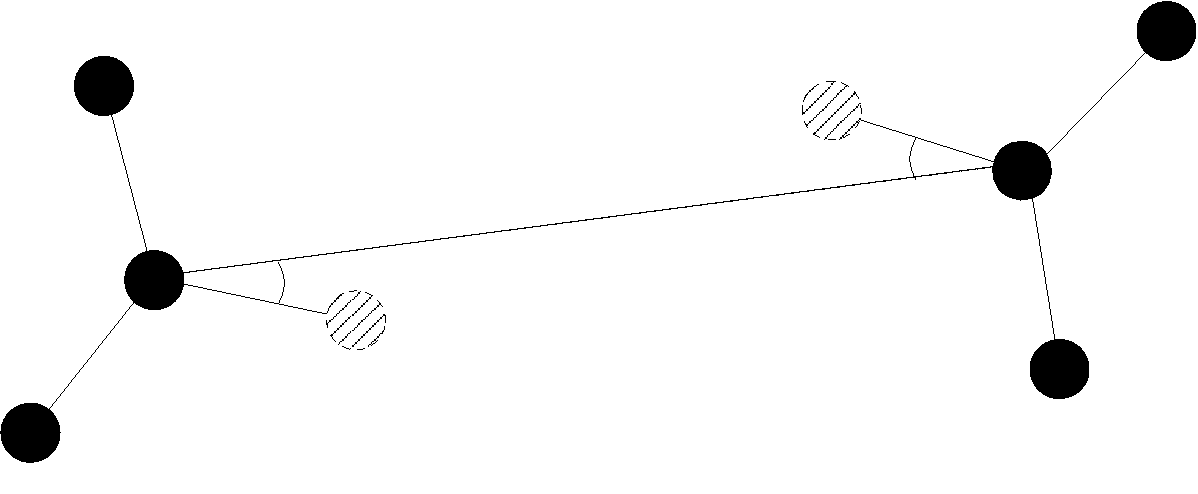
\includegraphics[height=8em]{figures/hbond}
\end{center}

Specifies a 12-10 Lennard-Jones interaction with angular dependence
between particles of the types \var{type1} and \var{type2}. These two
particles need two bonded partners oriented in a symmetric way. They
define an orientation for the central particle. The purpose of using
bonded partners is to avoid dealing with torques, therefore the
interaction does \emph{not} need the ROTATION feature. The angular
part of the potential minimizes the system when the two central beads
are oriented along the vector formed by these two particles. The
shaded beads on the image are virtual particles that are formed from
the orientation of the bonded partners, connected to the central
beads. They are used to define angles. The potential is of the form
\begin{equation}
  U(r_{ik},\theta_{jik},\theta_{ikn})=\epsilon\left[5\left(\frac{\sigma}r\right)^{12}-6\left(\frac{\sigma}{r}\right)^{10}\right]\cos^2\theta_{jik}\cos^2\theta_{ikn},
\end{equation}
where $r_{ik}$ is the distance between the two central beads, and each
angle defines the orientation between the direction of a central bead
(determined from the two bonded partners) and the vector
$\mathbf{r_{ik}}$. Note that the potential is turned off if one of the
angle is more than $\pi/2$. This way we don't end up creating a
minimum for an anti-parallel configuration.

Unfortunately, the bonded partners are not seeked dynamically. One has
to keep track of the relative positions of the particle IDs. This can
be done by setting the parameters \var{b1_a}, \var{b1_b}, \var{b2_a},
and \var{b2_b}. Say the first bead \var{type1} has particle ID
\var{n}, then one should set the simulation such as its two bonded
partners have particle IDs \var{n+b1_a} and \var{n+b1_b},
respectively. On a linear chain, for example, one would typically have
\var{b1_a=1} and \var{b1_b=-1} such that the central bead and its two
bonded partners have position IDs \var{n}, \var{n+1}, and \var{n-1},
respectively. This is surely not optimized, but once the simulation is
set correctly the algorithm is very fast.

The force can be capped using \lit{inter ljangleforcecap}. It might
turn out to be useful in some cases to keep this capping during the
whole simulation. This is due to the very sharp angular dependence for
small distance, compared to $\sigma$. Two beads might come very close
to each other while having unfavorable angles such that the
interaction is turned off. Then a change in the angle might suddenly
turn on the interaction and the system will blow up (the potential is
so steep that one would need extremely small time steps to deal with
it, which is not very clever for such rare events).

For instance, when modeling hydrogen bonds (N-H...O=C), one can avoid
simulating hydrogens and oxygens by using this potential. This comes
down to implementing a HBond potential between N and C atoms.

\todo{The contribution to the pressure is not yet implemented.}

\subsection{Smooth step interaction}
\index{smooth-step interaction|mainindex}
\index{interactions!smooth-step|mainindex}
\begin{essyntax}
  inter \var{type1} \var{type2}
  smooth-step \var{\sigma_1} \var{n} \var{\epsilon} \var{k_0}
  \var{\sigma_2} \var{r_\mathrm{cut}}
  \begin{features}
    \required{SMOOTH_STEP}
  \end{features}
\end{essyntax}
This defines a smooth step interaction between particles of the
types \var{type1} and \var{type2}, for which the potential is
\begin{equation}
  V(r)= \left(\var{\sigma_1}/d\right)^\var{n} + \epsilon/(1 + \exp\left[2k_0 (r - \sigma_2)\right])
\end{equation}
for $r<r_\mathrm{\var{cut}}$, and $V(r)=0$ elsewhere. With $n$ around
10, the first term creates a short range repulsion similar to the
Lennard-Jones potential, while the second term provides a much softer
repulsion. This potential therefore introduces two length scales, the
range of the first term, $\sigma_1$, and the range of the second one,
$\sigma_2$, where in general $\sigma_1<\sigma_2$.

\subsection{BMHTF potential}
\index{BMHTF interaction|mainindex}
\index{interactions!BMHTF|mainindex}
\begin{essyntax}
  inter \var{type1} \var{type2}
  bmhtf-nacl \var{A} \var{B} \var{C} \var{D} \var{\sigma} \var{r_\mathrm{cut}}
  \begin{features}
    \required{BMHTF_NACL}
  \end{features}
\end{essyntax}
This defines an interaction with the {\em short-ranged part} of the
Born-Meyer-Huggins-Tosi-Fumi potential between particles of the types
\var{type1} and \var{type2}, which is often used to simulate NaCl
crystals. The potential is defined by:
\begin{equation}
  V(r)= \var{A}\exp\left[\var{B}(\var{\sigma} - \var{r})\right] -
  \var{C} \var{r}^{-6} - \var{D} \var{r}^{-8} + \epsilon_\mathrm{shift},
\end{equation}
where $\epsilon_\mathrm{shift}$ is chosen such that
$V(\var{r_\mathrm{cut}})=0$. For $r\ge \var{r_\mathrm{cut}}$, the
$V(r)=0$.

For NaCl, the parameters should be chosen as follows:

\begin{tabular}{r|l|l|l|l|l}
  types & \var{A} (\unitfrac{kJ}{mol}) & \var{B} ($\unit{\AA^{-1}}$) &
  \var{C} ($\unit{\AA^6}$\unitfrac{kJ}{mol}) & \var{D}
  $\unit{\AA^8}$\unitfrac{kJ}{mol} & \var{\sigma} (\unit{\AA}) \\
  \hline
  Na-Na & 25.4435 & 3.1546 &  101.1719 &    48.1771 & 2.34 \\
  Na-Cl & 20.3548 & 3.1546 &  674.4793 &   837.0770 & 2.755 \\
  Cl-Cl & 15.2661 & 3.1546 & 6985.6786 & 14031.5785 & 3.170 \\
\end{tabular}

The cutoff can be chosen relatively freely because the potential
decays fast; a value around 10 seems reasonable.

In addition to this short ranged interaction, one needs to add a
Coulombic, long--ranged part. If one uses elementary charges, \ie a
charge of $q=+1$ for the Na--particles, and $q=-1$ for the
Cl--particles, the corresponding prefactor of the Coulomb interaction
is $\approx 1389.3549 \AA\,kJ/mol$.

\subsection{Morse interaction}
\index{Morse interaction|mainindex}
\index{interactions!Morse|mainindex}

\begin{essyntax}
  inter \var{type1} \var{type2} morse
  \var{\epsilon} \var{\alpha} \var{r_\mathrm{min}} \var{r_\mathrm{cut}}
  \begin{features}
    \required{MORSE}
  \end{features}
\end{essyntax}
This defines an interaction using the Morse potential between
particles of the types \var{type1} and \var{type2}. It serves similar
purposes as the Lennard-Jones potential, but has a deeper minimum,
around which it is harmonic.  This models the potential energy in a
diatomic molecule.  This potential allows capping the force using
\texttt{inter morseforcecap}, see section~\ref{sec:forcecap}.

For $r < \var{r_\mathrm{cut}}$, this potential is given by
\begin{equation}
  V(r)=\var{\epsilon}\left(\exp\left[-2 \var{\alpha} \left(r - \var{r_\mathrm{min}}\right)\right]
    - 2\exp\left[-\alpha\left(r - r_\mathrm{min}\right)\right]\right) -
  \epsilon_\mathrm{shift},
\end{equation}
where \var{\epsilon_\mathrm{shift}} is again chosen such that
$V(\var{r_\mathrm{cut}})=0$. For $r\ge \var{r_\mathrm{cut}}$, the $V(r)=0$.

\subsection{Buckingham interaction}
\index{Buckingham interaction|mainindex}
\index{interactions!Buckingham|mainindex}

\begin{essyntax}
  inter \var{type1} \var{type2} buckingham
  \var{A} \var{B} \var{C} \var{D}
  \var{r_\mathrm{cut}} \var{r_\mathrm{discont}} \var{\epsilon_\mathrm{shift}}
  \begin{features}
    \required{BUCKINGHAM}
  \end{features}
\end{essyntax}
This defines a Buckingham interaction between particles of the types
\var{type1} and \var{type2}, for which the potential is given by
\begin{equation}
  V(r)= A\exp(-B r) - Cr^{-6} - Dr^{-4} + \var{\epsilon_\mathrm{shift}}
\end{equation}
for $\var{r_\mathrm{discont}} < r < \var{r_\mathrm{cut}}$. Below \var{r_\mathrm{discont}},
the potential is linearly continued towards $r=0$, similarly to force capping,
see below. Above $r=\var{r_\mathrm{cut}}$, the potential is $0$. This potential
allows capping the force using \lit{inter buckforcecap}, see
section~\ref{sec:forcecap}.

\subsection{Soft-sphere interaction}
\index{soft-sphere interaction|mainindex}
\index{interactions!soft-sphere|mainindex}

\begin{essyntax}
  inter \var{type1} \var{type2}
  soft-sphere \var{a} \var{n} \var{r_\mathrm{cut}} \var{r_\mathrm{offset}}
  \begin{features}
    \required{SOFT_SPHERE}
  \end{features}
\end{essyntax}
This defines a soft sphere interaction between particles of the types
\var{type1} and \var{type2}, which is defined by a single power law:
\begin{equation}
  V(r)=a\left(r-r_\mathrm{\var{offset}}\right)^{-n}
\end{equation}
for $r<\var{r_\mathrm{cut}}$, and $V(r)=0$ above. There is no shift
implemented currently, which means that the potential is discontinuous
at $r=\var{r_\mathrm{cut}}$. Therefore energy calculations should be
used with great caution.

\subsection{Gay-Berne interaction}
\index{Gay-Berne interaction|mainindex}
\index{interactions!Gay-Berne|mainindex}

\begin{essyntax}
  inter \var{type1} \var{type2} gay-berne
  \var{\epsilon_0} \var{\sigma_0} \var{r_\mathrm{cutoff}}
  \var{k1} \var{k2} \var{\mu} \var{\nu}
  \begin{features}
    \required{ROTATION}
  \end{features}
\end{essyntax}
This defines a Gay-Berne potential for prolate and oblate particles
between particles of the types \var{type1} and \var{type2}. The
Gay-Berne potential is an anisotropic version of the classic
Lennard-Jones potential, with orientational dependence of the range
\var{\sigma_0} and the well-depth \var{\epsilon_0}.

Assume two particles with orientations given by the unit vectors
$\mathbf{\hat{u}}_i$ and $\mathbf{\hat{u}}_j$ and intermolecular vector
$\mathbf{r} = r\mathbf{\hat{r}}$. If $r<r_\mathrm{\var{cut}}$, then the
interaction between these two particles is given by
\begin{equation}
  V(\mathbf{r}_{ij}, \mathbf{\hat{u}}_i, \mathbf{\hat{u}}_j) = 4
  \epsilon(\mathbf{\hat{r}}_{ij}, \mathbf{\hat{u}}_i,
  \mathbf{\hat{u}}_j) \left( \tilde{r}_{ij}^{-12}-\tilde{r}_{ij}^{-6}
  \right),
\end{equation}
otherwise $V(r)=0$. The reduced radius is
\begin{equation}
  \tilde{r}=\frac{r - \sigma(\mathbf{\hat{r}},
    \mathbf{\hat{u}}_i, \mathbf{\hat{u}}_j)+\sigma_0}{\sigma_0},
\end{equation}
\begin{equation}
  \sigma( \mathbf{\hat{r}}, \mathbf{\hat{u}}_i,
  \mathbf{\hat{u}}_j) = \sigma_{0} \left\{ 1 - \frac{1}{2} \chi \left[
      \frac{ \left( \mathbf{\hat{r}} \cdot \mathbf{\hat{u}}_i +
          \mathbf{\hat{r}} \cdot \mathbf{\hat{u}}_j \right)^{2} }
      {1 + \chi \mathbf{\hat{u}}_i \cdot \mathbf{\hat{u}}_j } +
      \frac{ \left( \mathbf{\hat{r}} \cdot \mathbf{\hat{u}}_i -
          \mathbf{\hat{r}} \cdot \mathbf{\hat{u}}_j \right)^{2} }
      {1 - \chi \mathbf{\hat{u}}_i \cdot \mathbf{\hat{u}}_j}
    \right] \right\}^{-\frac{1}{2}}
\end{equation}
and
\begin{multline}
  \epsilon(\mathbf{\hat{r}}, \mathbf{\hat{u}}_i,
  \mathbf{\hat{u}}_j) = \\
  \epsilon_0 \left( 1- \chi^{2}(\mathbf{\hat{u}}_i
    \cdot \mathbf{\hat{u}}_j) \right)^{-\frac {\nu}{2}} \left[1-\frac
    {\chi'}{2} \left( \frac { (\mathbf{\hat{r}} \cdot
        \mathbf{\hat{u}}_i+ \mathbf{\hat{r}} \cdot
        \mathbf{\hat{u}}_j)^{2}} {1+\chi' \, \mathbf{\hat{u}}_i \cdot
        \mathbf{\hat{u}}_j }+ \frac {(\mathbf{\hat{r}} \cdot
        \mathbf{\hat{u}}_i-\mathbf{\hat{r}} \cdot
        \mathbf{\hat{u}}_j)^{2}} {1-\chi' \, \mathbf{\hat{u}}_i \cdot
        \mathbf{\hat{u}}_j } \right) \right]^{\mu}.
\end{multline}
The parameters $\chi = \left(k_1^{2} - 1\right)/\left(k_1^{2} +
  1\right)$ and $\chi' = \left(k_2^{1/\mu} -
  1\right)/\left(k_2^{1/\mu} + 1\right)$ are responsible for the
degree of anisotropy of the molecular properties.  \var{k_1} is the
molecular elongation, and \var{k_2} is the ratio of the potential well
depths for the side-by-side and end-to-end configurations.  The
exponents \var{\mu} and \var{\nu} are adjustable parameters of the
potential.  Several Gay-Berne parametrizations exist, the original one
being $\var{k_1} = 3$, $\var{k_2} = 5$, $\var{\mu} = 2$ and $\var{\nu}
= 1$.

\subsection{Tabulated interaction}
\index{tabulated interaction|mainindex}
\index{interactions!tabulated|mainindex}
\label{sec:tabnonbonded}

\begin{essyntax}
  inter \var{type1} \var{type2} tabulated \var{filename}%
  \begin{features}
    \required{TABULATED}
  \end{features}
\end{essyntax}

This defines an interaction between particles of the types \var{type1} and
\var{type2} according to an arbitrary tabulated pair potential. \var{filename}
specifies a file which contains the tabulated forces and energies as a function
of the separation distance. The tabulated potential allows capping the force
using \lit{inter tabforcecap}, see section~\ref{sec:forcecap}.

At present the required file format is simply an ordered list separated by
whitespace. The data reader first looks for a {\tt \#} character and begins
reading from that point in the file. Anything before the {\tt \#} will be
ignored.

The first three parameters after the {\tt \#} specify the number of data points
$N_\mathrm{points}$ and the minimal and maximal tabulated separation distances
$r_\mathrm{min}$ and $r_\mathrm{max}$. The number of data points obviously should
be an integer, the two other can be arbitrary positive doubles. Take care when
choosing the number of points, since a copy of each lookup table is kept on each
node and must be referenced very frequently. The maximal tabulated separation
distance also acts as the effective cutoff value for the potential.

The remaining data in the file should consist of n data triples $r$, $F(r)$ and
$V(r)$. $r$ gives the particle separation, $V(r)$ specifies the interaction
potential, and $F(r)= -V'(r)/r$ the force (note the factor $1/r$!). The values
of $r$ are assumed to be equally distributed between $r_\mathrm{min}$ and
$r_\mathrm{max}$ with a fixed distance of
$(r_\mathrm{max}-r_\mathrm{min})/(N_\mathrm{points}-1)$; the distance values $r$ in
the file are ignored and only included for human readability.

\subsection{Tunable-slip boundary interaction}
\index{Tunable-slip boundary interaction|mainindex}
\index{interactions!Tunable-slip boundary interactions|mainindex}
\begin{essyntax}
  inter \var{type1} \var{type2}
  tunable_slip \var{T} \var{\gamma_L} \var{r_\mathrm{cut}} \var{\delta t}
  \var{v_x} \var{v_y} \var{v_z}
  \begin{features}
    \required{TUNABLE_SLIP}
  \end{features}
\end{essyntax}
Simulating microchannel flow phenomena like the Plane Poiseuille and
the Plane Couette Flow require accurate boundary conditions. There are
two main boundary conditions in use:

\begin{enumerate} 
\item \emph{slip boundary condition} which means that the flow
  velocity at the the hydrodynamic boundaries is zero.
\item \emph{partial-slip boundary condition} which means that the flow 
  velocity at the hydrodynamic boundaries does not vanish.
\end{enumerate}

In recent years, experiments have indicated that the no-slip boundary
condition is indeed usually not valid on the micrometer
scale. Instead, it has to be replaced by the {\em {partial-slip
    boundary condition}}
\begin{displaymath}
\delta_B \: \: \partial_{{\bf n}} v_{\parallel}|_{{\bf r}_B} =
v_{\parallel}|_{{\bf r}_B},
\end{displaymath}
where $v_{\parallel}$ denotes the tangential component of the velocity
and $\partial_{{\bf n}} v_{\parallel}$ its spatial derivative normal
to the surface, both evaluated at the position ${\bf r}_B$ of the
so-called {\em hydrodynamic boundary}.  This boundary condition is
characterized by two effective parameters, namely (i) the slip length
$\delta_B$ and (ii) the hydrodynamic boundary ${\bf r}_B$.

Within the approach of the tunable-slip boundary interactions it is
possible to tune the slip length systematically from full-slip to
no-slip.  A coordinate-dependent Langevin-equation describes a viscous
layer in the vicinity of the channel walls which exerts an additional
friction on the fluid particles.  \var{T} is the temperature,
\var{\gamma_L} the friction coefficient and \var{r_\mathrm{cut}} is
the cut-off radius of this layer. \var{\delta t} is the timestep of
the integration scheme. With \var{v_x} \var{v_y} and \var{v_z} it is
possible to give the layer a reference velocity to create a Plane
Couette Flow.  Make sure that the cutoff radius \var{r_\mathrm{cut}}
is larger than the cutoff radius of the constraint Lennard-Jones
interactions. Otherwise there is no possibility that the particles
feel the viscous layer.

This method was tested for Dissipative Particle Dynamics but it is
intended for mesoscopic simulation methods in general. Note, that to
use tunable-slip boundary interactions you have to apply \textbf{two}
plane cell constraints with Lennard-Jones in addition to the
tunable-slip interaction. Make sure that the cutoff radius
\var{r_\mathrm{cut}} is larger than the cutoff radius of the
constraint Lennard-Jones interactions. Otherwise there is no
possibility that the particles feel the viscous layer.  Please read
reference \cite{smiatek08a} before using this interaction.

\subsection{Capping the force during warmup}
\label{sec:forcecap}

\begin{essyntax}
  \variant{1} inter ljforcecap \alt{\var{F_\mathrm{max}} \asep individual}
  \variant{2} inter morseforcecap \alt{\var{F_\mathrm{max}} \asep individual}
  \variant{3} inter buckforcecap \alt{\var{F_\mathrm{max}} \asep individual}
  \variant{4} inter tabforcecap \alt{\var{F_\mathrm{max}} \asep individual}
  \begin{features}
    \required[\variant{1}]{LENNARD_JONES}
    \required[\variant{2}]{MORSE}
    \required[\variant{3}]{BUCKINGHAM}
    \required[\variant{4}]{TABULATED}
  \end{features}  
\end{essyntax}

Non-bonded interactions are often used to model the hard core
repulsion between particles. Most of the potentials in the section are
therefore singular at zero distance, and forces usually become very
large for distances below the particle size. This is not a problem
during the simulation, as particles will simply avoid overlapping.
However, creating an initial dense random configuration without
overlap is often difficult.

By artificially capping the forces, it is possible to simulate a
system with overlaps. By gradually raising the cap value
\var{F_\mathrm{max}}, possible overlaps become unfavorable, and the
system equilibrates to a overlap free configuration.

This command will cap the force to \var{F_\mathrm{\var{max}}}, \ie for
particle distances which would lead to larger forces than
\var{F_\mathrm{max}}, the force remains at \var{F_\mathrm{max}}.
Accordingly, the potential is replaced by replaced by $r
\var{F_\mathrm{max}}$. Particles placed exactly on top of each other
will be subject to a force of magnitude \var{F_\mathrm{max}} along
the first coordinate axis.

The force capping is switched off by setting $\var{F_\mathrm{max}}=0$.
Note that force capping always applies to all interactions of the
corresponding type (\eg all Lennard-Jones interactions) regardless of
the particle types.

If instead of a force capping value, the string ``individual'' is
given, the force capping can be set individually for each
interaction. The capping radius is in this case not derived from the
potential parameters, but is given by an additional signal floating
point parameter to the interaction.

\section{Bonded interactions}
\label{sec:inter-bonded}
\index{bonded interactions|mainindex}
\index{interactions!bonded|mainindex}

\begin{essyntax*}
  inter \var{bondid}
  \opt{\var{interaction}}
  \opt{\var{parameters}}
\end{essyntax*}

\index{bonded interaction type id} Bonded interactions are identified
by their \emph{bonded interaction type identificator} \var{bondid},
which is a non-negative integer.  The \lit{inter} \var{bondid} command
is used to specify the type and parameters of a bonded interaction,
which applies to all particles connected explicitely by this bond
using the \keyword{part} command (see section \vref{tcl:part}).
Therefore, defining a bond between two particles always involves two
steps: defining the interaction and applying it. Assuming that two
particles with ids 42 and 43 already exist, one can create \eg a
FENE-bond between them using
\begin{tclcode}
  inter 1 fene 10.0 2.0
  part 42 bond 1 43
\end{tclcode}
If a FENE-bond with the same interaction parameters is required between several
particles (\eg in a simple chain molecule), one can use the sampe type \var{id}:
\begin{tclcode}
  inter 1 fene 10.0 2.0
  part 42 bond 1 43; part 43 bond 1 44 
\end{tclcode}

Bonds can have more than just two bond partners. For the \keyword{inter} command
that does not play a role as it only specifies the parameters, only when
applying the bond using the \keyword{bond} particle, the number of involved
particles plays a role. The number of involved particles and their order, if
important, is nevertheless specified here for completeness.

\subsection{FENE bond}
\index{FENE bond|mainindex}
\index{interactions!FENE|mainindex}

\begin{essyntax}
  inter \var{bondid}
  fene
  \var{K} \var{\Delta r_\mathrm{max}} \opt{\var{r_0}}
\end{essyntax}
This creates a bond type with identificator \var{bondid} with a
FENE (finite extension nonlinear expander) interaction. This is a
rubber-band-like, symmetric interaction betweeen two particles with
prefactor \var{K}, maximal stretching \var{\Delta r_\mathrm{max}} and
equilibrium bond length \var{r_0}.  The bond potential diverges at a
particle distance $r=\var{r_0}-\var{\Delta r_\mathrm{max}}$ and
$r=\var{r_0}+\var{\Delta r_\mathrm{max}}$. It is given by
\begin{equation}
  V(r) = -\frac{1}{2} \var{K} \var{\Delta r_\mathrm{max}}^2\ln \left[ 1 - \left(
      \frac{r-\var{r_0}}{\var{\Delta r_\mathrm{max}}} \right)^2 \right].
\end{equation}

\subsection{Harmonic bond}
\index{harmonic bond|mainindex}
\index{interactions!harmonic|mainindex}

\begin{essyntax}
  inter \var{bondid}
  harmonic \var{K} \var{R}
\end{essyntax}
This creates a bond type with identificator \var{bondid} with a
classical harmonic potential. It is a symmetric interaction between two
particles. The potential is minimal at particle distance $r=R$, and the
prefactor is $K$. It is given by
\begin{equation}
  V(r) = \frac{1}{2} K \left( r - R \right)^2
\end{equation}

\subsection{Subtracted Lennard-Jones bond}
\index{subtracted Lennard-Jones bond|mainindex}
\index{interactions!subtracted Lennard-Jones|mainindex}

\begin{essyntax}
  inter \var{bondid}
  subt_lj
  \var{reserved} \var{R}
\end{essyntax}
This creates a ``bond'' type with identificator \var{bondid}, which
acts between two particles and actually subtracts the Lennard-Jones interaction
between the involved particles.  The first parameter, \var{reserved} is a dummy
just kept for compatibility reasons. The second parameter, \var{R}, is used as a
check: if any bond length in the system exceeds this value, the program
terminates. When using this interaction, it is worthwhile to consider
capping the Lennard-Jones potential appropriately so that round-off errors can
be avoided.

This interaction is useful when using other bond potentials which already
include the short--ranged repulsion. This often the case for force fields or in
general tabulated potentials.

\subsection{Rigid bonds}
\index{rigid bond|mainindex}
\index{interactions!rigid bond|mainindex}
\index{RATTLE}

\begin{essyntax}
  inter \var{bondid}
  rigid_bond
  \var{constrained_bond_distance} \var{positional_tolerance} 
  \var{velocity_tolerance}
\end{essyntax}

\todo{Docs}

\subsection{Bond-angle interactions}
\index{bond-angle interactions|mainindex}
\index{interactions!bond-angle|mainindex}
\label{sec:angle}

\begin{essyntax}
  inter \var{bondid}
  angle \var{K} \opt{\var{\phi_0}}
  \begin{features}
    \required{BOND_ANGLE_HARMONIC} \required{BOND_ANGLE_COSINE} or
    \required{BOND_ANGLE_COSSQUARE}
  \end{features}
\end{essyntax}

This creates a bond type with identificator \var{bondid}
with an angle dependent potential. This potential is defined between
three particles. The particle for which the bond is created, is the
central particle, and the angle $\phi$ between the vectors from this
particle to the two others determines the interaction.  \var{K} is the
bending constant, and the optional parameter \var{phi_0} is the
equilibirum bond angle in radian ranging from 0 to $\pi$.  If this
parameter is not given, it defaults to $\var{\phi_0} = \pi$, which
corresponds to a stretched configuration. For example, for a bond
defined by
\begin{code}
  part \$p_2 bond 4 \$p_1 \$p_3
\end{code}
the minimal energy configurations are the following:
\begin{center}
  \setlength{\unitlength}{3000sp}
  \begin{picture}(8381,2684)(1570,-5393)
    \thinlines
    \put(2701,-4561){\circle*{450}}
    \put(3601,-4561){\circle*{450}}
    \put(4501,-4561){\circle*{450}}
    \put(7021,-4561){\circle*{450}}
    \put(7921,-4561){\circle*{450}}
    \put(7921,-3661){\circle*{450}}
    \thicklines
    \put(2701,-4561){\line( 1, 0){1800}}
    \put(7021,-4561){\line( 1, 0){900}}
    \put(7921,-4561){\line( 0, 1){900}}
    \put(5761,-2831){\line( 0,-1){2500}}

    \put(2701,-5191){\makebox(0,0)[b]{$p_1$}}
    \put(3601,-5191){\makebox(0,0)[b]{$p_2$}}
    \put(4501,-5191){\makebox(0,0)[b]{$p_3$}}
    \put(7021,-5191){\makebox(0,0)[b]{$p_1$}}
    \put(8371,-3751){\makebox(0,0)[b]{$p_3$}}
    \put(7921,-5191){\makebox(0,0)[b]{$p_2$}}
    \put(7921,-2941){\makebox(0,0)[b]{\keyword{inter 4 angle 1.0 [expr [PI]/2]}}}
    \put(3601,-2941){\makebox(0,0)[b]{\keyword{inter 4 angle 1.0 [PI]}}}
  \end{picture}%
\end{center}

For the potential acting between the three particles, different choices are
possible, which have to be activated in \texttt{myconfig.h}
\begin{itemize}
\item Harmonic bond angle potential (requires feature BOND_ANGLE_HARMONIC):\\
  A classical harmonic potential,
  \begin{equation}
    V(\phi) = \frac{K}{2} \left(\phi - \phi_0\right)^2.
  \end{equation}
  Unlike the two following variants, this potential has a kink at
  $\phi=\phi_0+\pi$ and accordingly a discontinuity in the force, and should
  therefore be used with caution.
\item Cosine bond angle potential (requires feature BOND_ANGLE_COSINE):\\
  \begin{equation}
    V(\alpha) = K \left[1 - \cos(\phi - \phi0)\right]
  \end{equation}
  Around $\phi_0$, this potenial is close to a harmonic one (both are
  $1/2(\phi-\phi_0)^2$ in leading order), but it is periodic and smooth for all
  angles $\phi$.
\item Cosine square bond angle potential (requires feature
  BOND_ANGLE_COSSQUARE):\\
  \begin{equation}
    V(\alpha) = \frac{K}{2} \left[\cos(\phi) - \cos(\phi_0)\right]^2
  \end{equation}
  This form is used for example in the GROMOS96 force field. The potential is
  $1/8(\phi-\phi_0)^4$ around $\phi_0$, and therefore much flatter than the
  two potentials before.
\end{itemize}

\subsection{Dihedral interactions}
\index{dihedral interactions|mainindex}
\index{interactions!dihedral|mainindex}
\label{sec:dihedral}

\begin{essyntax}
  inter \var{bondid} dihedral \var{n} \var{K} \var{p}
\end{essyntax}

This creates a bond type with identificator \var{bondid}
with a dihedral potential, \ie a four-body-potential. In the following,
let the particle for which the bond is created be particle $p_2$, and
the other bond partners $p_1$, $p_3$, $p_4$, in this order, \ie
\lit{part $p_2$ bond bondid $p_1$ $p_3$ $p_4$}. Then, the
dihedral potential is given by
\begin{equation}
  V(\phi) = \var{K}\left[1 - \cos(\var{n}\phi - \var{p})\right],
\end{equation}
where \var{n} is the multiplicity of the potential (number of minimas)
and can take any integer value (typically from 1 to 6), $p$ is a phase
parameter and \var{K} is the bending constant of the potential. $\phi$
is the dihedral angle between the particles defined by the particle
quadrupel $p_1$, $p_2$, $p_3$ and $p_4$, \ie the angle between the
planes defined by the particle triples $p_1$, $p_2$ and $p_3$ and
$p_2$, $p_3$ and $p_4$:
\begin{center}
  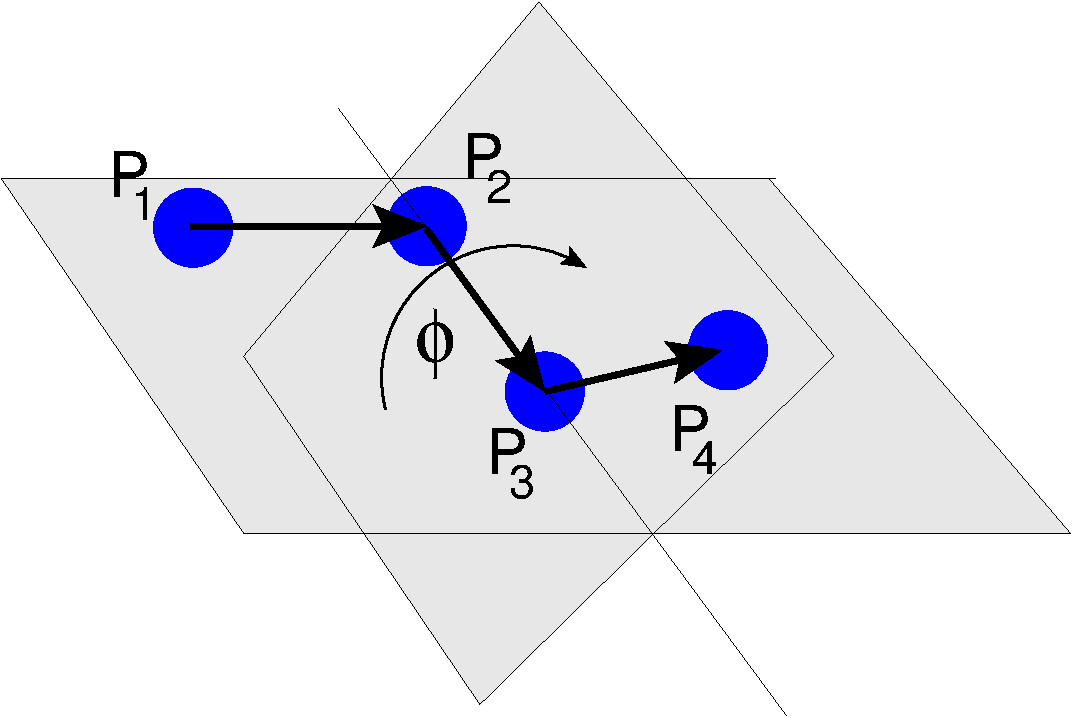
\includegraphics[height=8em]{figures/dihedral-angle}
\end{center}
Together with appropriate Lennard-Jones interactions, this potential
can mimic a large number of atomic torsion potentials.

If you enable the feature OLD_DIHEDRAL, then the old, less
general form of the potential is used:
\begin{equation}
  V(\phi) = \var{K}\left[1 + \var{p}\,\cos(\var{n}\phi)\right],
\end{equation}
where $p$ is rather a phase factor and can only take values $p=\pm 1$.

\subsection{Tabulated bond interactions}
\index{tabulated bond interactions|mainindex}
\index{interactions!tabulated bond|mainindex}

\begin{essyntax}
    \variant{1} inter \var{bondid}
    tabulated bond \var{filename}
    \variant{2} inter \var{bondid}
    tabulated angle \var{filename}
    \variant{3} inter \var{bondid}
    tabulated dihedral \var{filename}
\end{essyntax}

This creates a bond type with identificator \var{bondid} with a
two-body bond length (\variant{1}), three-body angle (\variant{2}) or four-body
dihedral (\variant{3}) tabulated potential. The tabulated forces and energies
have to be provided in a file \var{filename}, which is formatted identically as
the files for non-bonded tabulated potentials (see
section\ref{sec:tabnonbonded}).

The potential is calculated as follows:
\begin{itemize}
\item Variant~\variant{1} is a two body interaction depending on the distance of
  two particles. The force acts in the direction of the connecting vector
  between the particles. The bond breaks above the tabulated range, but for
  distances smaller than the tabulated range, a linear extrapolation based on
  the first two tabulated force values is used.
\item Variant~\variant{2} is a three-body angle interaction similar to the
  \texttt{angle} potential (see section~\ref{sec:angle}).  It is assumed that
  the potential is tabulated for all angles between 0 and $ \pi $, where 0
  corresponds to a stretched polymer, and just as for the tabulated pair
  potential, the forces are scaled with the inverse length of the connecting
  vectors. The force on particles $p_1$ and $p_3$ (in the notation of
  section~\ref{sec:angle}) acts perpendicular to the connecting vector between
  the particle and the center particle $p_2$ in the plane defined by the three
  particles. The force on the center particle $p_2$ balances the other two
  forces.
\item Variant~\variant{3} tabulates a torsional dihedral angle potential (see
  section~\ref{sec:dihedral}). It is assumed that the potential is tabulated for
  all angles between 0 and $2\pi$. \em{This potential is not tested yet! Use on
    own risk, and please report your findings and eventually necessary fixes.}
\end{itemize}

\subsection{Virtual bonds}

\begin{essyntax}
  inter \var{bondid} virtual_bond
\end{essyntax}

This creates a virtual bond type with identificator \var{bondid}, \ie
a pair bond without associated potential or force. It can used to specify
topologies and for some analysis that rely on bonds, or \eg for bonds that
should be displayed in VMD.

\section{Coulomb interaction}
\label{sec:inter-electrostatics}
\index{Coulomb interactions|mainindex}
\index{interactions!Coulomb|mainindex}

Electrostatic interactions are very computation time-intensive. \es{} features
some state-of-the-art algorithms to deal with these interactions as efficiently
as possible, but almost all of them require some knowledge to use them properly.
Uneducated use can result in completely unphysical simulations.

\begin{essyntax}
  \variant{1} inter coulomb 0.0
  \variant{2} inter coulomb \opt{\var{l_B} \var{method}} \opt{\var{parameters}}
  \variant{3} inter coulomb
\end{essyntax}

This command defines how \es deals with electrostatic interactions.

Variant \variant{1} completely disables Coulomb interactions hence
deactivating the electrostatic subsystem, while variant \variant{2}
sets up one of the methods described below to treat electrostatic
interactions. \var{l_B} denotes the Bjerrum length, which measures the
strength of the electrostatic interaction.  For a pair of particles at
distance $r$ with charge $q$ each, the interaction is given by
\begin{equation}
  U^C(r)=l_B k_B T\frac{q^2}{r}.
\end{equation}
Using the electrostatic interaction also requires to assign charges to the
particles. This is done using the \texttt{part} command to set the charge
\texttt{q}, \eg

\begin{tclcode}
  inter coulomb 1.0 p3m tune accuracy 1e-4
  part 0 q 1.0; part 1 q -1.0
\end{tclcode}

Variant \variant{3} returns the current parameters of the coulomb
interaction as a tcl-list using the same syntax as used to setup the
method, \eg
\begin{tclcode}
  {coulomb 1.0 p3m 7.75 8 5 0.1138 0.0}
  {coulomb epsilon 0.1 n_interpol 32768 mesh_off 0.5 0.5 0.5}
\end{tclcode}

\subsection{P3M}
\index{P3M method|mainindex}
\index{interactions!P3M|mainindex}

\begin{essyntax}
  \variant{1} inter coulomb p3m \var{r_\mathrm{cut}} \var{mesh} \var{cao} \var{alpha}
  \variant{2}inter magnetic p3m \var{r_\mathrm{cut}} \var{mesh} \var{cao} \var{alpha}
\end{essyntax}

The variant \variant{1}  activates the P3M method to handle the electrostatic interactions (charge-charge), whereas
the variant \variant{2} activates the P3M method to handle the magnetostatic interactions (magnetic dipole-dipole) (aka dipolar-P3M).

For electrostatics the interaction is:
\begin{equation}
  U^{C-P3M} = \ell_B k_B T \frac{q_1 q_2}{r}
\end{equation}
Here $\ell_B = e_o^2 / (4 \pi \epsilon k_B T)$ is the Bjerrum length.

For magnetostatics the interaction is:
\begin{equation}
  U^{D-P3M} = \ell_{Bm} k_B T \left( \frac{(\vec{\mu}_i \cdot \vec{\mu}_j)}{r^3} 
  - \frac{3  (\vec{\mu}_i \cdot \vec{r}_{ij})  (\vec{\mu}_j \cdot \vec{r}_{ij}) }{r^5} \right)
\end{equation}
Here $\vec{r}_{ij}=\vec{r}_{i}-\vec{r}_{j}$, and  $\ell_{Bm}$ is a non dimensional parameter similar to the Bjerrum length in electrostatics which
 can help to tune the effect of the medium on the magnetic interaction between two magnetic dipoles.

Make sure that you know the relevance of the P3M parameters before
using P3M! If you are not sure, read the following references
\cite{ewald21,hockney88,kolafa92,deserno98,deserno98a,deserno00,deserno00a,cerda08a}.

\subsubsection{Tuning P3M}
\begin{essyntax}
  inter \alt{coulomb \asep magnetic}  p3m \alt{tune \asep tunev2}
  accuracy \var{accuracy}\\
  \opt{r_cut \var{r_\mathrm{cut}}}
  \opt{mesh \var{mesh}}
  \opt{cao \var{cao}}
  \opt{alpha \var{\alpha}}
\end{essyntax}

Make sure you know how to tune p3m parameters before using the
automatic tuning feature.

For the charge-charge interaction the function utilizes the analytic expression of the error estimate
for the P3M method in the book of Hockney and Eastwood \cite[eqn
8.23]{hockney88} in order to obtain the rms error in the force for a
system of N randomly distributed particles in a cubic box.  For the
real space error the estimate of Kolafa and Perram\cite{kolafa92} is
used. For the magnetic case, magnetic dipole-dipole interaction, the expressions of the error estimate
for the dipolar-P3M are those written in Cerda et al. \cite{cerda08a}. At this moment, the P3M methods only 
work for cubic boxes.  The magnetostatics must be activated enabling the flag "MAGNETOSTATICS" in the file
"myconfig.h".

The two tuning methods follow different methods for determining the
optimal parameter. While the \keyword{tune} version simply tests
different values on a grid in the parameter space, the
\keyword{tunev2} version uses a bisection to determine the optimal
parameters. In general, for small systems the \keyword{tune} version
is faster, while for large systems \keyword{tunev2} is faster. The
results of \keyword{tunev2} are always at least as good as the
parameters achievable from the \keyword{tune} version, and normally
the obtained accuracy is much closer to the desired value.

During execution the tuning routines report the parameter sets tested,
the corresponding k-space and real-space errors and timings needed for
force calculations (the setmd variable \var{timings} controls the
number of test force calculations). Since the error depends on
\var{r_\mathrm{cut}}/\var{box\_l} and \var{\alpha}\var{box\_l} the
output is given in these units.

Note that any previous settings of \var{r_\mathrm{cut}}, \var{cao} and
\var{mesh} will be remembered. So if you want to retune your
electrostatics, \eg after a major system change, you should use
\begin{code}
inter \alt{coulomb \asep magnetic}  \var{l_B} p3m tune accuracy \var{acc} r_cut 0 mesh 0 cao 0
\end{code}

Some additional p3m parameters have preset value
\begin{tclcode}
 epsilon = metallic
\end{tclcode}
The dielectric constant of the surrounding medium, metallic
(i.e.infinity) or some finite positive number.
\begin{tclcode}
 n_interpol = 32768
\end{tclcode}
Number of interpolation points for the charge assignment function.
When this is set to 0, interpolation is turned off.
\begin{tclcode}
 mesh_off = 0.5 0.5 0.5
\end{tclcode}
Offset of the first mesh point from the lower left corner of the
simulation box in units of the mesh constant. As soon as p3m is turned
on the additional parameters can be changed with:
\begin{code}
inter coulomb \var{parameter_name} \var{value}+
\end{code}

If only magnetic dipoles are present in the sytem (no charges present), it is advisable to turn off
the flag "ELECTROSTATICS" in the file "myconfig.h" to improve the performance of the program.  Mixed systems 
containing magnetic dipoles and charges can be simulated without problem  enabling both flags: "ELECTROSTATICS" and 
"MAGNETOSTATICS". For each kind of particle one should use the prefered algorithm. For magnetic dipole-dipole interactions
the only algorithm implemented at this moment is the dipolar-P3M. In principle there is no problem to use a non P3M method
to deal with charges (see folowing sections) while one uses dipolar-P3M to deal with the magnetic dipoles. In case you use P3M for both charges and magnetic dipoles,
make sure that you tune each P3M method (coulomb/magnetic) to the desired accuracy. 


\subsection{Debye-H\"uckel potential}
\index{Debye-H\"uckel potential|mainindex}
\index{interactions!Debye-H\"uckel|mainindex}

\todo{How is the cutoff handled? Why is this not a normal short-raged
  potential?}
\begin{essyntax}
  inter coulomb dh \var{\kappa} \var{r_\mathrm{cut}}
\end{essyntax}

Defines the electrostatic potential by
\begin{equation}
  U^{C-DH} = \ell_B k_B T \frac{q_1 q_2 exp(-\kappa r)}{r}
\end{equation}

For $\kappa = 0$, this corresponds to the plain coulomb potential.

\subsection{MMM2D}
\index{MMM2D method|mainindex}
\index{interactions!MMM2D|mainindex}

\begin{essyntax}
 inter coulomb mmm2d \var{maximal\_pairwise\_error}
 \opt{\var{fixed\_far\_cutoff}}
 \opt{dielectric \var{\epsilon_t} \var{\epsilon_m} \var{\epsilon_b}}
 \opt{dielectric-contrasts \var{\Delta_t} \var{\Delta_b}}
\end{essyntax}
MMM2D coulomb method for systems with periodicity 1 1 0. Needs the
layered cell system. The performance of the method depends on the
number of slices of the cell system, which has to be tuned manually.
It is automatically ensured that the maximal pairwise error is smaller
than the given bound. The far cutoff setting should only be used for
testing reasons, otherwise you are more safe with the automatical
tuning. If you even don't know what it is, do not even think of
touching the far cutoff. For details on the MMM family of algorithms,
refer to appendix \vref{chap:mmm}.

The last two, mutually exclusive arguments ``dielectric'' and
``dielectric-constants'' allow to specify dielectric contrasts at the
upper and lower boundaries of the simulation box. The first form
specifies the respective dielectric constants in the media, which
however is only used to calculate the contrasts. That is, specifying 
$\epsilon_t=\epsilon_m=\epsilon_b=\text{const}$ is always identical to
$\epsilon_t=\epsilon_m=\epsilon_b=1$. The second form specifies only
the dielectric contrasts at the boundaries, that is
$\Delta_t=\frac{\epsilon_m-\epsilon_t}{\epsilon_m+\epsilon_t}$ and
$\Delta_b=\frac{\epsilon_m-\epsilon_b}{\epsilon_m+\epsilon_b}$. Using
this form allows to choose $\Delta_{t/b}=-1$, corresponding to
metallic boundary conditions.

\subsection{MMM1D}
\index{MMM1D method|mainindex}
\index{interactions!MMM1D|mainindex}

\begin{essyntax}
  \variant{1}
  inter coulomb mmm1d \var{switch\_radius}
  \opt{\var{bessel\_cutoff}} \var{maximal\_pairwise\_error}

  \variant{2}
  inter coulomb mmm1d tune \var{maximal\_pairwise\_error}
\end{essyntax}
MMM1D coulomb method for systems with periodicity 0 0 1. Needs the
nsquared cell system (see section \vref{sec:cell-systems}). The first
form sets parameters manually. The switch radius determines at which
xy-distance the force calculation switches from the near to the far
formula. If the Bessel cutoff is not explicitly given, it is
determined from the maximal pairwise error, otherwise this error only
counts for the near formula. The second, tuning form just takes the
maximal pairwise error and tries out a lot of switching radii to find
out the fastest one. If this takes too long, you can change the value
of the setmd variable \keyword{timings}, which controls the number of
test force calculations. For details on the MMM family of algorithms,
refer to appendix \vref{chap:mmm}.

\subsection{Maggs' method}
\index{Maggs' method|mainindex}
\index{interactions!Maggs' method|mainindex}

\begin{essyntax}
  inter coulomb
  maggs \var{f\_mass} \var{mesh} \var{field\_friction}
  \opt{yukawa \var{kappa} \var{r_\mathrm{cut}}}
\end{essyntax}

This is an implementation of the instantaneous 1/r Coulomb interaction
\begin{equation}
  U = \ell_B k_B T \frac{q_1 q_2}{r}
\end{equation}
as the potential of mean force between charges which are dynamically
coupled to a local electromagnetic field.

\begin{arguments}
\item[\var{f\_mass}] is the mass of the field degree of freedom and equals
  to the square root of the inverted speed of light.
\item[\var{mesh}] is the number of mesh points for the interpolation
  of the electromagnetic field.
\item[\var{field\_friction}] is the value of the friction coefficient
  for the transversal field degrees of freedom (reserved for future
  development).
\end{arguments}
Unphysical self--energies that arise as a result of the lattice
interpolation of charges, are corrected by a subtraction scheme based
either on the exact lattice Green's function or the combination of the
direct subtraction scheme plus the Yukawa subtraction scheme (second
method).

For the case of Yukawa screened simulation (second method) one has to
enter screening parameter \var{kappa} and the cut-off of the Yukawa
potential \var{r_\mathrm{cut}}.

\subsection{ELC}
\index{ELC method|mainindex}
\index{interactions!ELC method|mainindex}

\begin{essyntax}
  inter coulomb elc \var{maximal\_pairwise\_error} \var{gap\_size}
  \opt{\var{far\_cutoff}}
\end{essyntax}
This is a special procedure that converts a 3d method, \ie P3M at the
moment, to a 2d method, in computational order N. This is definitely
faster than MMM2D for larger numbers of particles (>400 at reasonable
accuracy requirements). The maximal pairwise error is the LUB error of
the force between any two charges without prefactors (see the papers).
The gap size gives the height of the empty region between the system
box and the neighboring artificial images (again, see the paper).
\es{} does not make sure that the gap is actually empty, this is the
users responsibility. The method will compute fine of the condition is
not fulfilled, however, the error bound will not be reached. Therefore
you should really make sure that the gap region is empty (e. g. by
constraints). The far cutoff finally is only intended for testing and
allows to directly set the cutoff. In this case, the maximal pairwise
error is ignored. The periodicity has to be set to 1 1 1 still, and
the 3d method has to be set to epsilon metallic, i.e.  metallic
boundary conditions. For details, see appendix \vref{chap:mmm}.

Make sure that you read the papers on ELC before using it !!!
\todo{references}

\section{Other interaction types}
\label{sec:inter-other}

\subsection{Fixing the center of mass}
\begin{essyntax}
  inter \var{typeid1} \var{typeid1} comfixed \var{flag}
\end{essyntax}
This interaction type applies a constraint on particles of type
\var{typeid1} such that during the integration the center of mass of
these particles is fixed. This is accomplished as follows: The sum of
all the forces acting on particles of type \var{typeid1} are
calculated. These include all the forces due to other interaction
types and also the thermostat. Next a force equal in magnitude, but in
the oppositte direction is applied on the particles. This force is
divided equally on all the particles of type \var{typeid1}, since
currently there is no mass concept in \es. Note that the syntax of the
declaration of comfixed interaction requires the same particle type to
be input twice. If different particle types are given in the input,
the program exits with an error message. \var{flag} can be set to 1
(which turns on the interaction) or 0 (to turn off the interaction).

\subsection{Pulling particles apart}
\begin{essyntax}
  inter \var{typeid1} \var{typeid2}
  comforce \var{flag} \var{dir} \var{force} \var{fratio}
\end{essyntax}
The comforce interaction type enables one to pull away particle groups
of two different types. It is mainly designed for pulling experiments
on bundles. Within a bundle of molecules of type number \var{typeid1}
lets mark one molecule as of type \var{typeid2}. Using comforce one
can apply a force such that t2 can be pulled away from the bundle. The
\var{comforce_flag} is set to 1 to turn on the interaction, and to 0
otherwise. The pulling can be done in two different directions. Either
parallel to the major axis of the bundle ($\var{dir} = 0$) or
perpendicular to the major axis of the bundle ($\var{dir} = 1$).
\var{force} is used to set the magnitude of the force.  \var{fratio}
is used to set the ratio of the force applied on particles of
\var{typeid1} vs. \var{typeid2}. This is useful if one has to keep the
total applied force on the bundle and on the target molecule the same.
A force of magnitude \var{force} is applied on \var{typeid2}
particles, and a force of magnitude (\var{force} * \var{fratio}) is
applied on \var{typeid1} particles.

%%% Local Variables:
%%% mode: latex
%%% TeX-master: "ug"
%%% End:

\chapter{Setting up the system}
\label{chap:setup}

\section{\texttt{setmd}: Setting global variables.}
\newescommand{setmd}

\begin{essyntax}
\variant{1} setmd \var{variable}
\variant{2} setmd \var{variable} \opt{\var{value}}+
\end{essyntax}
\todo{Explain '+' in intro.}

Variant \variant{1} returns the value of the \es global variable
\var{variable}, variant \variant{2} can be used to set the variable
\var{variable} to \var{value}. The following global variables can be
set:

%% List-environment for the description of the global variables
\newenvironment{globvar}{
  \begin{list}{}{
      \setlength{\rightmargin}{1em}
      \setlength{\leftmargin}{2em}
      \setlength{\partopsep}{0pt}
      \setlength{\topsep}{1ex}
      \setlength{\parsep}{0.5ex}
      \setlength{\listparindent}{-1em}
      \setlength{\labelwidth}{0.5em}
      \setlength{\labelsep}{0.5em}
      \renewcommand{\makelabel}[1]{%
        \index{##1@\texttt{##1} (global variable)|mainindex}%
        \index{global variables!\texttt{##1}|mainindex}%
        \texttt{##1}%
      }
    }
  }{
  \end{list}
}
\newcommand{\ro}{\emph{read-only}}

\todo{Better throw some out (\eg switches)?}
\todo{Missing: lattice_switch, dpd_tgamma, n_rigidbonds}
\todo{Which commands can be used to set the \emph{read-only}
  variables?}
\begin{globvar}
\item[box_l] (double[3]) Simulation box length.
  \todo{document what happens to the particles when \keyword{box_l} is
    changed!}
\item[cell_grid] (int[3], \ro) Dimension of the inner
  cell grid.
\item[cell_size] (double[3], \ro) Box-length of a cell.
\item[dpd_gamma] (double, \ro) Friction constant for the
  DPD thermostat.
\item[dpd_r_cut] (double, \ro) Cutoff for DPD thermostat.
\item[gamma] (double, \ro) Friction constant for the
  Langevin thermostat.
\item[integ_switch] (int, \ro) Internal switch which integrator to
  use.
\item[local_box_l] (int[3], \ro) Local simulation box length of the
  nodes.
\item[max_cut] (double, \ro) Maximal cutoff of real space
  interactions.
\item[max_num_cells] (int) Maximal number of cells for the link cell
  algorithm.  Reasonable values are between 125 and 1000, or for some
  problems (\var{n_total_particles} / \var{n_nodes}).
\item[max_part] (int, \ro) Maximal identity of a particle.
  \emph{This is in general not related to the number of particles!}
\item[max_range] (double, \ro) Maximal range of real space
  interactions: \var{max_cut} + \var{skin}.
\item[max_skin] (double, \ro) Maximal skin to be used for the link
  cell/verlet algorithm. This is the minimum of \var{cell_size} -
  \var{max_range}. \todo{???}
\item[min_num_cells] (int) \todo{???} Minimal number of cells for the
  link cell algorithm. Reasonable values range in $1e-6 N^2$ to $1e-7
  N^2$. In general just make sure that the Verlet lists are not
  incredibly large. By default the minimum is 0, but for the automatic
  P3M tuning it may be wise to larger values for high particle
  numbers.
\item[n_layers] (int, \ro) Number of layers in cell structure LAYERED
  (see section \vref{sec:cell-systems}).
\item[n_nodes] (int, \ro) Number of nodes.
\item[n_part] (int, \ro) Total number of particles.
\item[n_part_types] (int, \ro) Number of particle types that were
  used so far in the \keyword{inter} command (see chapter{tcl:inter}).
\item[node_grid] (int[3]) 3D node grid for real space domain
  decomposition (optional, if unset an optimal set is chosen
  automatically).
\item[nptiso_gamma0] (double, \ro)\todo{Docs missing.}
\item[nptiso_gammav] (double, \ro)\todo{Docs missing.}
\item[npt_p_ext] (double, \ro) Pressure for NPT simulations.
\item[npt_p_inst] (double) Pressure calculated during an
  NPT_isotropic integration.
\item[piston] (double, \ro) Mass off the box when using NPT_isotropic
  integrator.
\item[periodicity] (bool[3]) Specifies periodicity for the three
  directions. If the feature PARTIAL_PERIODIC is set, this variable
  can be set to (1,1,1) or (0,0,0) at the moment.  If not it is
  readonly and gives the default setting (1,1,1).\todo{Correct?}
\item[skin] (double) Skin for the Verlet list.
\item [temperature] (double, \ro) Temperature of the
  simulation.
\item[thermo_switch] (double, \ro) Internal variable which thermostat
  to use. 
\item[time] (double) The simulation time.
\item[time_step] (double) Time step for MD integration.
\item[timings] (int) Number of timing samples to take into account if
  set.\todo{???}
\item[transfer_rate] (int, \ro) Transfer rate for VMD connection. You
  can use this to transfer any integer value to the simulation from
  VMD.
\item[verlet_flag] (bool) Indicates whether the Verlet list will be
  rebuild. The program decides this normally automatically based on
  your actions on the data.
\item[verlet_reuse] (double) Average number of integration steps the
  verlet list has been re-used.
\end{globvar}

\section{\texttt{thermostat}: Setting up the thermostat}
\newescommand{thermostat}

\begin{essyntax}
  \variant{1} thermostat off
  \variant{2} theormstat \var{method} \opt{\var{parameter}}+
\end{essyntax}
\todo{Include docs from \texttt{thermostat.h}!}
Change thermostat settings.

\section{\texttt{nemd}: Setting up non-equilibrium MD}
\newescommand{nemd}

\begin{essyntax}
  \variant{1}nemd \var{method} \var{parameter} 
  \variant{2}nemd off
  \variant{3}nemd profile
  \variant{4}nemd viscosity
\end{essyntax}
\todo{Include docs from \texttt{nemd.h}!}
\todo{Put \texttt{nemd profile|viscosity} into \texttt{analyze}?}  
Use NEMD (Non Equilibrium Molecular Dynamics) to simulate a system
under shear.

\section{\texttt{cellsystem}: Setting up the cell system}
\label{sec:cell-systems}
\newescommand{cellsystem}

This section deals with the flexible particle data organization of
\es.  Due to different needs of different algorithms, \es is able to
change the organization of the particles in the computer memory,
according to the needs of the used algorithms. For details on the
internal organization, refer to section
\vref{sec:internal-particle-organization}.

\subsection{Domain decomposition}
\index{domain decomposition}
\begin{essyntax}
  cellsystem domain_decomposition \opt{-no_verlet_list}
\end{essyntax}
This selects the domain decomposition cell scheme, using Verlet lists
for the calculation of the interactions. If you specify
\keyword{-no_verlet_list}, only the domain decomposition is used, but
not the Verlet lists.

The domain decomposition cellsystem is the default system and suits
most applications with short ranged interactions. The particles are
divided up spatially into small compartments, the cells, such that the
cell size is larger than the maximal interaction range. In this case
interactions only occur between particles in adjacent cells. Since the
interaction range should be much smaller than the total system size,
leaving out all interactions between non-adjacent cells can mean a
tremendous speed-up. Moreover, since for constant interaction range,
the number of particles in a cell depends only on the density. The
number of interactions is therefore of the order N instead of order
$N^2$ if one has to calculate all pair interactions.

\subsection{N-squared}
\begin{essyntax}
  cellsystem nsquare 
\end{essyntax}
This selects the very primitive nsquared cellsystem, which calculates
the interactions for all particle pairs. Therefore it loops over all
particles, giving an unfavorable computation time scaling of $N^2$.
However, algorithms like MMM1D or the plain Coulomb interaction in the
cell model require the calculation of all pair interactions.

In a multiple processor environment, the nsquared cellsystem uses a
simple particle balancing scheme to have a nearly equal number of
particles per CPU, \ie $n$ nodes have $m$ particles, and $p-n$ nodes
have $m+1$ particles, such that $n*m+(p-n)*(m+1)=N$, the total number
of particles. Therefore the computational load should be balanced
fairly equal among the nodes, with one exception: This code always
uses one CPU for the interaction between two different nodes. For an
odd number of nodes, this is fine, because the total number of
interactions to calculate is a multiple of the number of nodes, but
for an even number of nodes, for each of the $p-1$ communication
rounds, one processor is idle.

E.g. for 2 processors, there are 3 interactions: 0-0, 1-1, 0-1.
Naturally, 0-0 and 1-1 are treated by processor 0 and 1, respectively.
But the 0-1 interaction is treated by node 1 alone, so the workload
for this node is twice as high. For 3 processors, the interactions are
0-0, 1-1, 2-2, 0-1, 1-2, 0-2. Of these interactions, node 0 treats 0-0
and 0-2, node 1 treats 1-1 and 0-1, and node 2 treats 2-2 and 1-2.

Therefore it is highly recommended that you use nsquared only with an
odd number of nodes, if with multiple processors at all. 

\subsection{Layered cell system}
\begin{essyntax}
  cellsystem layered \var{n_layers}
\end{essyntax}

This selects the layered cell system, which is specifically designed
for the needs of the MMM2D algorithm. Basically it consists of a
nsquared algorithm in x and y, but a domain decomposition along z, i.
e. the system is cut into equally sized layers along the z axis. The
current implementation allows for the cpus to align only along the z
axis, therefore the processor grid has to have the form 1x1xN.
However, each processor may be responsible for several layers, which
is determined by \var{n\_layers}, i. e. the system is split into
N*\var{n\_layers} layers along the z axis. Since in x and y direction
there are no processor boundaries, the implementation is basically
just a stripped down version of the domain decomposition cellsystem.

%%% Local Variables: 
%%% mode: latex
%%% TeX-master: "ug"
%%% End: 

\chapter{Running the simulation}
\label{chap:run}

\section{\texttt{integrate}: Running the simulation}
\eslabel{integrate}

\begin{essyntax}
  \variant{1} integrate \var{steps}
  \variant{2} integrate set \var{method} \opt{\var{parameter}}+
\end{essyntax}

\todo{Docs missing!}
\todo{Which integrators do exist?}

\section{\texttt{change_volume}: Changing the box volume}
\eslabel[change-volume]{change_volume}

\begin{essyntax}
  \variant{1} change_volume \var{V_new} 
  \variant{2} change_volume \var{L_new} \alt{x \asep y \asep z \asep xyz}
\end{essyntax}
Changes the volume of either a cubic simulation box to the new volume
\var{V_new} or its given x-/y-/z-/xyz-extension to the new box-length
\var{L_new}, and isotropically adjusts the particles coordinates as
well. The function returns the new volume of the deformed simulation
box.

\section{Stopping particles}
\eslabel{stopParticles}
\eslabel[stop-particles]{stop_particles}

\begin{essyntax}
  \variant{1} stopParticles
  \variant{2} stop_particles
\end{essyntax}
Halts all particles in the current simulation, setting their
velocities and forces to zero. Variant \variant{2} does not provide
feedback on the execution status.

\section{\texttt{velocities}: Setting the velocities}
\eslabel{velocities}
\begin{essyntax}
  velocities \var{v_max} 
  \opt{start \var{part_id}} 
  \opt{count \var{N_T}}
\end{essyntax}
Sets the velocities of the particles with particle ID (see The part
command) between \var{part_id} and \var{part_id}+\var{N_T}
(defaults to '0' \& '[setmd npart]-\var{part_id}') to a random vector
with length in [-vmax,vmax], and returns the absolute value of the
total velocity assigned.

\section{\texttt{invalidate_system}}
\eslabel[invalidate-system]{invalidate_system}
\begin{essyntax}
  invalidate_system
\end{essyntax}
\todo{Documentation not up to date!}

Forces a system re-init which, among others, causes the integrator to
also update the forces at its beginning (instead of re-using the
values from the previous integration step).  This is particularly
necessary to ensure continuity after setting a checkpoint:
\texttt{integrate} - \texttt{set_checkpoint} - \texttt{integrate} has
only one call to \todo{???}???, while \texttt{read_checkpoint} -
\texttt{integrate} has two at the beginning of the 2nd integrate
(because loading a new system from disk typically requires
re-initializing the system), and since ??? also uses the thermostat
which in turn draws random numbers, the two situations do not end up
at the same segment of the random number sequence, all random events
will therefore slightly differ.  To prevent this, simply include a
call to invalidate_system upon setting the checkpoint (this is being
done automatically if using tcl_checkpoint_set and
tcl_checkpoint_read beginning with v1.1 of \es{}), because in that
case both scenarios will call ??? twice at the beginning of the second
integration phase thus having their random number sequences in total
sync. The C implementation is invalidate_system.



%%% Local Variables: 
%%% mode: latex
%%% TeX-master: "ug"
%%% End: 

\chapter{Analysis}
\label{chap:analysis}


%%% Local Variables: 
%%% mode: latex
%%% TeX-master: "ug"
%%% End: 

\chapter{Input / Output}
\label{cha:io}

\section{\texttt{blockfile}}
In a nutshell: The blockfile command is provided for saving and
restoring the current state of \es, e. g. for creating and using
checkpoints. Hence you can transfer all accessible informations to and
from disk from and to \es.

\begin{itemize}
 \item
\begin{code}
set out [open "|gzip -c - > checkpoint.block.gz" "w"]
blockfile $out write variable all
blockfile $out write interactions
blockfile $out write random
blockfile $out write bitrandom
blockfile $out write particles "id pos type q v f" all
blockfile $out write bonds all
blockfile $out write configs
close $out 
\end{code}

This example writes all variables accessible by The setmd command, all
interactions known to The inter command, the full current state of the
random number generator (The t\_random command or The bit\_random
command), all informations (i.e. id, position, type-number, charge,
velocity, forces, bonds) on all particles, and all particle
configurations appended (using e. g. analyze append) for
offline-analysis purposes to the file 'checkpoint.block.gz' which is
even being compressed on-the-fly (if you don't want that, use
\codebox{set out [open "checkpoint.block" "w"]}
instead).
Note that interactions must be stored before particles before bonding
informations, as for the bonds to be set all particles and all
interactions must already be known to \es{}.

 \item
\begin{tclcode}
set in [open "|gzip -cd checkpoint.block.gz" "r"]
while { [blockfile $in read auto] != "eof" } {}
close $in 
\end{tclcode}
This is basically all you need to restore the informations in the
blockfile (again, if you don't have a compressed file, use
\begin{code}
set out [open "checkpoint.block" "r"]
\end{code}
instead) overwriting the current settings in \es{}.
\end{itemize}
And now the full documentation on how The blockfile command actually
works:

\tclcommand{blockfile}
{
  \var{channel} 
  read|write 
  start|end|variable|auto|toend
  \opt{\var{param}}
}

blockfile allows for convienent access to a block format structured
file \var{channel}. Some of the possible actions are:
\begin{enumerate}
 \item
\begin{code}
blockfile <channel>  write start <tag> 
\end{code}
which writes a start "\{" and the title of the block given by
\var{tag}.
 \item
\begin{code}
blockfile <channel> write end 
\end{code}
just writes a "\}" to \var{channel}.
 \item
\begin{code}
blockfile <channel> write variable {<varname1> <varname2> ...}
\end{code}
writes the variables \var{varname1}, \var{varname2},..., which are
known to The setmd command (a list can be found in Global variables),
to \var{channel}. When reading the block, all variables with names
listed in blockfile\_variable\_blacklist are ignored.
 \item
\begin{code}
blockfile <channel> write variable all
\end{code}
  will write all variables known to The setmd command to \var{channel}.
 \item
\begin{code}
blockfile <channel> write tclvariable {<varname1> <varname2> ...}
\end{code}
writes the tcl global variables \var{varname1}, \var{varname2},..., to
\var{channel}. Global variables are those declared in the top scope or
those declared global in procedures. When reading the block, all
variables with names listed in blockfile\_tclvariable\_blacklist are
ignored.
 \item
\begin{code}
blockfile <channel> write tclvariable all
\end{code}
will write all global variables to \var{channel}. The predefined
globals from Tcl (tcl\_version, argv, argv0, tcl\_interactive,
auto\_oldpath, errorCode, auto\_path, errorInfo, auto\_index, env,
tcl\_pkgPath, tcl\_patchLevel, argc, tcl\_libPath, tcl\_library and
tcl\_platform) are omitted.
 \item
\begin{code}
blockfile <channel> write tclvariable reallyall
\end{code}
  will even write those variables, which you probably almost never want...
 \item
\begin{code}
blockfile <channel> write particles <what> <range>
\end{code}
writes particle information in a standardized format to the file
\var{channel}. \var{what} can be any list of parameters that part
\var{x} print takes except for "bonds". Notice that if "id" or "pos"
is missing, this is added in the front to the list automatically.
\var{range} is a Tcl list of ranges which particles to write. The
range "all" is valid as well as a boundary of "end". For example
\begin{code}
 blockfile file10 write particles "id pos q" "all 0-end 0" 
\end{code}
  will write all particles two times to file10 and then particle 0 alone.
 \item
\begin{code}
 blockfile <channel> write interactions
\end{code}
  writes interactions information in a standardized format to the file \var{channel}.
 \item
\begin{code}
blockfile <channel> write bonds <range>
\end{code}
writes bonds information in a standardized format to the file
\var{channel}. The involved particles and bond types must exist and be
valid.
 \item
\begin{code}
blockfile <channel> write random
\end{code}
writes the full informations on the current state of the random number
generators on any node to the file \var{channel}. Using this
information, it is possible to recover the exact state the generators
were in at that moment.
 \item
\begin{code}
blockfile <channel> write seed
\end{code}
writes only the seed(s) which were used to initialize the random
number generators. Note that this information is not sufficient to
pick up the random sequences where they were left, because The
t\_random command also uses a table of previous random numbers to
determine the next one; to also save that information use
tcl\_blockfile\_write\_random.
 \item
\begin{code}
blockfile <channel> write bitrandom
\end{code}
writes the full informations on the current state of the R250 random
number generators on any node to the file \var{channel}. Using this
information, it is possible to recover the exact state the generators
were in at that moment.
 \item
\begin{code}
blockfile <channel> write bitseed
\end{code}
writes only the seed(s) which were used to initialize the bit random
number generators. Note that this information is not sufficient to
pick up the random sequences where they were left, because The
bit\_random command uses a huge matrix of integers whose bit-patterns
are XOR-ed to determine the next one; to also save that information
use tcl\_blockfile\_write\_bitrandom.
 \item
\begin{code}
blockfile <channel> write configs
\end{code}
writes the complete content of the 'configs'-array in statistics.c to
\var{channel}, thereby saving all particle configurations appended (e.
g. using analyze append) for analysis-purposes.  Using this
offline-analysis is quite easy: Just append regularly the current
configurations, include this command after the derivation of the last
time step, and blockfile read auto will load them later on resetting
'configs' to the state needed for most of the more complex
analyze-commands.
 \item
\begin{code}
blockfile <channel> read start 
\end{code}
  reads the start part of a block and returns the block title.
 \item
\begin{code}
blockfile <channel> read toend 
\end{code}
  reads the blocks data and returns it.
 \item
\begin{code}
blockfile <channel> read particles|interactions|bonds|variable
 |seed|random|bitrandom|configs
\end{code}
reads one block, checks wether it contains data of the given type and
reads it.
 \item
\begin{code}
blockfile <channel> read auto 
\end{code}
  reads in one block and does the following:
  \begin{enumerate}
  \item if a procedure blockfile\_read\_auto\_\var{tag} exists, this
    procedure takes over (\var{tag} is the first expression in the
    block). For most block types, at least all mentioned above, i. e.
    particles, interactions, bonds, seed, random, bitrandom, configs,
    and variable, the corresponding procedure will overwrite the
    current information with the information from the block.
  \item if the procedure does not exist, it returns \codebox{usertag
      <tag> <rest of block>}
  \item if the file is at end, it returns \codebox{eof}
  \end{enumerate}
\end{enumerate}
If \codebox{blockfile <channel> read auto} finds a block, it tries to
load the corresponding procedure as described above.
\codebox{blockfile <channel> read <block>} checks for a block with tag
\var{block} and then again executes the corresponding
blockfile\_read\_auto\_\var{tag}, if it exists.

If that fails, blockfile executes \codebox{blockfile\_arg1\_arg2}, if
it exists, with the all arguments given to blockfile. For example
\begin{code}
blockfile channel write particles "id pos" all 
\end{code}
results in the evaluation of
\begin{code}
blockfile\_write\_particles channel write particles "id pos" all 
\end{code}
If the next block in a blockfile is a particle block, e. g.
\begin{tclcode}
{particles {id pos type q}
           {0 27.251 62.31 58.707 1 1.0}
           {1 27.226 61.483 58.146 0 0.0}
}
\end{tclcode}	
\begin{code}
  blockfile <channel> read auto
\end{code}
will call
\begin{code}
blockfile_read_auto_particles <channel> read auto
\end{code}
, which then will delete all particles and insert the two particles
above.

In the contrary that means that for a new blocktype you will normally
implement two procedures:
\begin{tclcode}
blockfile_write_<tag> {channel write <tag> param...}
\end{tclcode}
which writes the block including the header and enclosing braces and
\begin{tclcode}
blockfile_read_auto_<tag> {channel "read" "auto"}
\end{tclcode}
which reads the block data and the closing brace. The parameters
"write", "read", "\var{tag}" and "auto" are regular parameters which
will always have the specified value. They occur just for technical
reasons.

\section{Using Checkpoints, saving configurations}
The following procedures may be used to save/restore checkpoints to
minimize the hassel involved when your simulations crashes after long
runs. The scripts are located in scripts/auxiliary.tcl and use The
blockfile command as file format.
\begin{itemize}
 \item
\begin{code}
checkpoint\_set <destination> [<\# of configs> [<tclvar>
 [<ia\_flag> [<var\_flag> [<ran\_flag]]]]]
\end{code}
creates a checkpoint with path/filename \var{destination} (compressed
if \var{destination} ends with '.gz'), saving the last \var{\# of
  configs} which have been appended using analyze\_append (defaults to
'all'), adds all tcl-embedded variables specified in the tcl-list
\var{tclvar} (defaults to '-'), all interactions (The inter command) /
\es{}-variables (The setmd command) / random-number-generator
informations (The t\_random command etc.) unless their respective
flags \var{ia\_flag} / \var{var\_flag} / \var{ran\_flag} are set to
'-'; you may however choose to only include certain \es{}-variables
(The setmd command) by providing their names as a tcl-list in place of
\var{var\_flag}.  When you're reading this, tcl\_checkpoint\_set will
be using The invalidate\_system command automatically; therefore
continuing an integration after setting a checkpoint or restarting it
there by reading one should make absolutely no difference anymore,
since the current state of the random number generator(s) is/are
completely (re)stored to (from) the checkpoint and the integrator is
forced to re-init the forces (incl. thermostat) no matter what.  It
may be a good choice to use filenames such as
'kremer\_checkpoint.[eval format 05 \$integration\_step]' or
'kremer\_checkpoint.029.gz' for \var{destination} because the command
stores all the names of checkpoints set to a file derived from
\var{destination} by replacing the very last suffix plus maybe '.gz'
with '.chk' (in the above examples: 'kremer\_checkpoint.chk') which is
used by tcl\_checkpoint\_read to restore all checkpoints.  Although
'checkpoint\_set \var{destination}' without the optional parameters
will store a complete checkpoint sufficient for re-starting the
simulation later on, you may run out of memory while trying to save a
huge number of timesteps appended (analyze\_append). Hence one should
rather only save those configurations newly added since the last
checkpoint, i.e. if a checkpoint is created every 100,000 steps while
a configuration is appended every 500 steps you may want to use
'checkpoint\_set \var{destination} 200' which saves the current
configuration, all interactions, all bonds, the precise state of the
random number generator(s), and the last 200 entries appended to
configs since the last checkpoint was created. Since
tcl\_checkpoint\_read reads in successively the checkpoints given in
the '.chk'-file, the configs-array will nevertheless be completely
restored to its original state although each checkpoint-file contains
only a fraction of the whole array.
 \item
\begin{code}
checkpoint\_read <origin>
\end{code}

restores all the checkpoints whose filenames are listed in
\var{origin} in the order given therein, consequently putting the
simulation into the state it was in when tc\_checkpoint\_set was
called. If parts of the configs array are given in the files listed in
\var{origin}, it is assumed that they represent a fraction of the
whole array.
 \item
\begin{code}
polyBlockWrite <path> <param\_list> <part\_list>
\end{code}
writes out the current '\es{}' configuration as an AxA-blockfile,
including parameters, interactions, particles, and bonds.  \var{path}
should contain the filename including the full path to it.
\var{param\_list} gives a tcl-list of the '\es{}'-parameters (out of )
to be saved; if an empty list '{}' is supplied, no parameters are
written. If 'all', all parameters available through The setmd command
are written. Defaults to the full parameter set.  \var{part\_list}
gives a string of the particle-properties (out of pos | type | q | v |
f) to be saved to disk; if an empty string ' "" 'is provided, no
particles, no bonds, and no interactions are written. Defaults (if
omitted) to all particle-properties.  Depending on the file-name's
suffix, the output will be compressed (if \var{path} ends with '.gz'),
too.  Note, that 'polyBlockWrite' in combination with
tcl\_convertMD2Deserno replaces the (undocumented) function 'polywr':
To save the current configuration to a Deserno-compatible file (e. g.
for use with 'poly2pdb') you may now use tcl\_polyBlockWrite to save
your current configuration to a blockfile, and convert that with
tcl\_convertMD2Deserno afterwards, or you directly write a
Deserno-compatible file by invoking
\begin{code}
convertMD2Deserno "-1" <output-filename>
\end{code}

out of \es to save your current active configuration.  However, this
last paragraph now has only historical meaning (see Writing pdb/psf
files).
 \item
\begin{code}
polyBlockWriteAll <destination> [<tcl-var> [<rdm> [<configs>]]]
\end{code}

does even more than tcl\_polyBlockWrite, i.e. it saves all current
interactions, particles, bonds, \es{}-variables to \var{destination},
but in addition it also saves the tcl-variables specified by
\var{tcl-var} (if 'all', then all the variables in the active script
are stored), it saves the state of the random number generator if
\var{rdm} is 'random' (= complete state) or 'seed' (= only the seeds),
and it saves all the particle configurations used for analysis
purposes if \var{configs} is all but '-'.  Using '-' as value usually
skips that entry.  With this one can set real checkpoints which should
reproduce the script-state as precisely as possible.
\end{itemize}

\section{The structured file format}
\label{sec:structured-file-format}

This describes the ASCII block format used for writing structured
files for analysis or storage. Basically the file consists of blocks
in curled braces, which have a single word title and some data. The
data itself may consist again of such blocks. An example is:
\begin{tclcode}
{file {Demonstration of the block format}
{variable epsilon {_dval_ 1} } 
{variable p3m_mesh_offset {_dval_ 5.0000000000e-01
 5.0000000000e-01 5.0000000000e-01 } } 
{variable node_grid {_ival_ 2 2 2 } } 
{end } }
\end{tclcode}

The format does not specify the number of whitespaces or which are
used as delimiters, space, tab and return are ok.

The keyword variable should be used to indicate that a variable
definition follows in the form \var{name} \var{data}. \var{data}
itself is a block with title \_ival\_ or \_dval\_ denoting integer
rsp. double values, which then follow in a whitespace separated list.
Such blocks can be read in conveniently using block\_read\_data and
written using block\_write\_data.

An example C-code generating the example above is:
\begin{tclcode}
// This file is part of the ESPResSo distribution
   (http://www.espresso.mpg.de).
// It is therefore subject to the ESPResSo license agreement which
   you accepted upon receiving the distribution
// and by which you are legally bound while utilizing this file in
   any form or way.
// There is NO WARRANTY, not even the implied warranty of
   MERCHANTABILITY or FITNESS FOR A PARTICULAR PURPOSE.
// You should have received a copy of that license along with this
   program;
// if not, refer to http://www.espresso.mpg.de/license.html where its
   current version can be found, or
// write to Max-Planck-Institute for Polymer Research, Theory Group,
   PO Box 3148, 55021 Mainz, Germany.
// Copyright (c) 2002-2006; all rights reserved unless otherwise
   stated.
#include "blockfile.h"

/*
  Demonstration of the use of the blockfile interface.
  Build using gcc -Wall -o test test.c -LLinux -lEspresso.
*/
int main()
{
  double epsilon = 1;
  double p3m_mesh_offset[3] = {.5, .5, .5};
  int    node_grid[3] = {2, 2, 2};

  FILE *f = fopen("demofile","w");
  block_writestart(f, "file");
  fprintf(f, "{Demonstration of the block format}\\n");

  /* variable epsilon */
  block_writestart(f, "variable");
  fprintf(f, "epsilon ");
  block_write_data(f, TYPE_DOUBLE, 1, &epsilon);
  block_writeend(f);
  fprintf(f, "\\n");

  /* variable p3m_mesh_offset */
  block_writestart(f, "variable");
  fprintf(f, "p3m_mesh_offset ");
  block_write_data(f, TYPE_DOUBLE, 1, p3m_mesh_offset);
  block_writeend(f);
  fprintf(f, "\\n");

\end{tclcode}
\begin{tclcode}
  /* variable node_grid */
  block_writestart(f, "variable");
  fprintf(f, "node_grid ");
  block_write_data(f, TYPE_DOUBLE, 1, node_grid);
  block_writeend(f);
  fprintf(f, "\\n");

  /* end tag */
  block_writestart(f, "end");
  block_writeend(f);

  block_writeend(f);
  fclose(f);
  return 0;
}
\end{tclcode}

\section{Writing pdb/psf files}
The PDB (Brookhaven Protein DataBase) format is a widely used format
for describing atomic configurations. PSF is a format that is used by
VMD to describe the topology of a PDB file. You need the PDB and PSF
files for example for IMD.
\begin{tclcode}
writepsf <file> { <N_P> <MPC> <N_CI> <N_pS> <N_nS> }|-molecule
\end{tclcode}
writes the current topology to the file <file> (here <file> is not a
channel since additional information cannot be written anyways).
\var{N\_P}, \var{MPC} and so on are parameters describing a system
consisting of equally long charged polymers, counterions and salt.
This information is used to set the residue name and can be used to
color the atoms in VMD. If you specify -molecule, the residue name is
taken from the molecule identity of the particle. Of course different
kinds of topologies can also be handled by modified versions of
writepsf.
\begin{code}
writepdb <file>
\end{code}
writes the corresponding particle data.
\begin{tclcode}
writepdbfoldchains <file> { < chain_start> <n_chains> <chain_length>
 <box_l> }
\end{tclcode}
Writes folded particle data where the folding is performed on chain
centers of mass rather than single particles. In order to fold in this
way the chain topology and box length must be specified. Note that
this method is outdated. Use writepdbfoldtopo instead.
\begin{tclcode}
writepdbfoldtopo <file> { <shift> } 
\end{tclcode}
Writes folded particle data where the folding is performed on chain
centers of mass rather than single particles. This method uses the
internal box length and topology information from espresso. If you
wish to shift particles prior to folding then supply the optional
shift information. Shift should be a three member tcl list consisting
of x, y, and z shifts respectively and each number should be a
floating point (ie with decimal point).

\section{Writing VTF files}
%\quickrefheading{Handling of VTF files}

There are two commands in \es{} that support writing files in the VMD
formats VTF, VSF and VCF.\footnote{A description of the format and a
  plugin to read the format in VMD is found in the subdirectory
  \texttt{vmdplugin/} of the \es{} source directory.} The commands can
be used to write the structure (\texttt{writevsf}) and coordinates
(\texttt{writevcf}) of the system to a single trajectory file (usually
with the extension \texttt{.vtf}), or to separate files (extensions
\texttt{.vsf} and \texttt{.vtf}).

\subsection{\texttt{writevsf}}

\tclcommand{writevsf}
{\var{channelId} \opt{<short|verbose>} \opt{radius <\var{radii}|auto>} 
  \opt{typedesc \var{typedesc}}}

Writes a structure block describing the system's structure to the
channel given by \var{channelId}. \var{channelId} must be an
identifier for an open channel such as the return value of an
invocation of \keyword{open}. The atom ids used in the file are not
necessarily identical to \es's particle ids. To get the atom id used
in the vtf file from an \es particle id, use the command
\keyword{vtfpid} described below. This makes it easy to write
additional structure lines to the file, e.g. to specify the
\texttt{resname} of particle compounds, like chains.  The output of
this command can be used for a standalone VSF file, or at the
beginning of a trajectory VTF file that contains a trajectory of a
whole simulation.

\begin{arguments}
\item[\opt{<short|verbose>}]
  Specify, whether the output is in a human-readable, but somewhat
  longer format (\keyword{verbose}), or in a more compact form
  (\keyword{short}). The default is \keyword{verbose}.
  
\item[\opt{radius <\var{radii}|auto>}]
  Specify the VDW radii of the atoms. \var{radii} is either
  \keyword{auto}, or a Tcl-list describing the radii of the different
  particle types. When the keyword \keyword{auto} is used and a
  Lennard-Jones interaction between two particles of the given type is
  defined, the radius is set to be $\frac{\sigma_{LJ}}{2}$ plus the LJ
  shift.  Otherwise, the radius $0.5$ is substituted. The default is
  \keyword{auto}.
  
  Example: \verb!writevsf $file radius {0 2.0 1 auto 2 1.0}!
  
\item[\opt{typedesc \var{typedesc}}]
  \var{typedesc} is a Tcl-list giving additional VTF atom-keywords to
  specify additional VMD characteristics of the atoms of the given type.
  If no description is given for a certain particle type, it defaults to
  \texttt{name \textit{name} type \textit{type}}, where \textit{name}
  is an atom name and \textit{type} is the type id.
  
  Example: \verb!writevsf $file typedesc {0 "name colloid" 1 "name pe"}!
\end{arguments}

\subsection{\texttt{writevcf}}
\tclcommand{writevcf}
{\var{channelId} \opt{<short|verbose>} \opt{<folded|absolute>}
  \opt{pids <\var{pids}|all>}}

Writes a coordinate (or timestep) block that contains all coordinates
of the system's particles to the channel given by \var{channelId}.
\var{channelId} must be an identifier for an open channel such as the
return value of an invocation of \keyword{open}.

\begin{arguments}
\item[\opt{<short|verbose>}] Specify, whether the output is in a
  human-readable, but somewhat longer format (\keyword{verbose}), or
  in a more compact form (\keyword{short}). The default is
  \keyword{verbose}.
  
\item[\opt{<folded|absolute>}] Specify whether the particle positions
  are written in absolute coordinates (\keyword{absolute}) or folded
  into the central image of a periodic system (\keyword{folded}). The
  default is \keyword{absolute}.
  
\item[\opt{pids <\var{pids}|all>}] Specify the coordinates of which
  particles should be written. If \keyword{all} is used, all
  coordinates will be written (in the ordered timestep format).
  Otherwise, \var{pids} has to be a Tcl-list specifying the pids of
  the particles. The default is \keyword{all}.
  
  Example: \verb!pids {0 23 42}!
  
\end{arguments}

\subsection{\texttt{vtfpid}}
\tclcommand{vtfpid}{\var{pid}}

If \var{pid} is the id of a particle as used in \es, this command
returns the atom id used in the VTF, VSF or VCF formats.


\section{\texttt{imd}: Online-visualisation with VMD}
IMD (Interactive Molecular Dynamics) is the protocol VMD uses to
communicate with a simulation. Tcl\_md implements this protocol to
allow online visual analysis of running simulations.

In IMD, the simulation acts as a data server. That means that a
simulation can provide the possibility of connecting VMD, but VMD need
not be connected all the time. You can watch the simulation just from
time to time.

In the following the setup up and using of IMD is described.

\subsection{IMD in the script}

In your simulation, the IMD connection is setup up using \codebox{imd
  connect <port>}

where \var{port} is an arbitrary port number (it has to be between
1024 and 65000). Normally \es{} will try to open port 10000, but the
port may be in use already by another \es{} simulation. In that case
it is a good idea to just try another port (see lj\_liquid.tcl).

Now while the simulation is running, you should execute
\begin{code}
imd positions <flag>
\end{code}
from time to time, which will transfer the current coordinates to VMD,
if it is connected. If not, nothing happens and imd connect just
consumes a small amount of CPU time. The optional flag argument can
take values -unfolded or -fold\_chains. By specifying -unfolded the
unfolded coordinates for each particle will be given to VMD.
Specifying -fold\_chains causes imd to call the routine
analyze\_fold\_molecules which folds chains according to their centers
of mass and retains bonding connectivity. Note that this routine
requires the chain structure to be specified first using the analyze
command.
\begin{code}
imd listen <seconds>
\end{code}
can be used to let the simulation wait for \var{seconds} seconds or
until IMD has connected. This is normally only useful in demo scripts,
if you want to see all frames of the simulation.

If your simulations terminates,
\begin{code}
imd disconnect
\end{code}

will terminate the IMD session. This is normally not only nice but
also the operating system will not free the port for some time, so
that without disconnecting for some 10 seconds you will not be able to
reuse the port.

Additionally, you have to provide VMD with the structural information
for your system. Therefore your program has to write out
psf-/pdb-files using tcl\_writepsf and tcl\_writepdb.

That hassle is greatly reduced by using the built-in auxiliary script
\begin{code}
prepare\_vmd\_connection [<filename> [<wait> [<start>]]]
\end{code}

which writes out the necessary psf-/pdb-files to \var{filename}.psf
and \var{filename}.pdb (default for <filename is 'vmd'), doing some
nice stuff such as coloring the molecules, bonds and counterions
appropriately, rotating your viewpoint, and connecting your system to
the visualization server. If \var{start} is 1 (the default), it does
all that by itself; otherwise it writes those steps out to a
script-file 'vmd\_start.script and waits for \var{wait} seconds
(default: 0) for you to connect.

\subsection{Using IMD in VMD}
So after your simulation runs and has written the psf/pdb files, you
start VMD. Then click on "Molecule", choose fileformat "psf and pdb",
and select your psf/pdb files in the corresponding entries. Now click
on "Load Molecule". You should see the snapshot you saved in the
psf/pdb files.

Then execute "imd connect \var{host} \var{port}", where \var{host} is
the host running the simulation and \var{port} is the port it listens
to. Note that VMD crashes, if you do that without loading the molecule
before .

For more information on how to use VMD to extract more information or
hide parts of configuration, see the VMD Quick Help.

\section{Errorhandling}
Errors in the parameters are detected as early as possible, and
hopefully self-explanatory error messages returned without any changes
to the data in the internal data of \es. This include errors such as
setting nonexistent properties of particles or simply misspelled
commands. These errors are returned as standard Tcl errors and can be
caught on the Tcl level via
\begin{tclcode}
catch {script} err 
\end{tclcode}
When run noninteractively, Tcl will return a nice stack backtrace
which allows to quickly find the line causing the error.

However, some errors can only be detected after changing the internal
structures, so that \es{} is left in a state such that integration is
not possible without massive fixes by the users. Especially errors
occuring on nodes other than the primary node fall under this
condition, for example a broken bond or illegal parameter
combinations.

For error conditions such as the examples given above, an Tcl error
message of the form
\begin{tclcode}
<Tcl error> background 0 {<error a>} {<error b>} 1 {<error c>}
\end{tclcode}
is returned. Following possibly a normal Tcl error message, after the
background keyword all severe errors are listed node by node,
preceeded by the node number. a special error is "<consent>", which
means that one of the slave nodes found exactly the same errors as the
master node. This happens mainly during the initialization of the
integrate, \eg if the time step is not set. In this case the error
message will be
\begin{tclcode}
background_errors 0 {time_step not set} 1 <consent> 
\end{tclcode}
In each case, the current action was not fulfilled, and possibly other
parts of the internal data also had to be changed to allow \es{} to
continue, so you should really know what you do if you try and catch
these errors.


%%% Local Variables: 
%%% mode: latex
%%% TeX-master: "ug"
%%% End: 

\chapter{Auxilliary commands}
\label{chap:aux}

\section{Writing VTF files}
%\quickrefheading{Handling of VTF files}

There are two commands in \es{} that support writing files in the VMD
formats VTF, VSF and VCF.\footnote{A description of the format and a
  plugin to read the format in VMD is found in the subdirectory
  \texttt{vmdplugin/} of the \es{} source directory.} The commands can
be used to write the structure (\texttt{writevsf}) and coordinates
(\texttt{writevcf}) of the system to a single trajectory file (usually
with the extension \texttt{.vtf}), or to separate files (extensions
\texttt{.vsf} and \texttt{.vtf}).

\subsection{\texttt{writevsf}}

\tclcommand{writevsf}
{\var{file} [<short|verbose>] [<\var{radii}|auto>] [typedesc \var{typedesc}]}

Writes a structure block describing the system's structure to
\var{file}. The atom ids used in the file are identical to \es's
particle ids.  This makes it easy to write additional structure lines
to the file, e.g. to specify the \texttt{resname} of particle
compounds, like chains.  The output of this file can be used in a
standalone VSF file, or at the beginning of a trajectory VTF file that
contains a trajectory of a whole simulation.

\begin{tcloptions}
  \option{<short|verbose>}
  Specify, whether the output is in a human-readable, but somewhat
  longer format (\keyword{verbose}), or in a more compact form
  (\keyword{short}). The default is \keyword{verbose}.
  
  \option{<radius \var{radii}|auto>}
  Specify the VDW radii of the atoms. \var{radii} is either
  \keyword{auto}, or a Tcl-list describing the radii of the different
  particle types. When the keyword \keyword{auto} is used and a
  Lennard-Jones interaction between two particles of the given type is
  defined, the radius is set to be $\frac{\sigma_{LJ}}{2}$ plus the LJ
  shift.  Otherwise, the radius $0.5$ is substituted. The default is
  \keyword{auto}.
  
  Example: \verb!writevsf "show.tcl" radius {{0 2.0} {1 auto} {2 1.0}}!
  
  \option{typedesc \var{typedesc}}
  \var{typedesc} is a Tcl-list giving additional VTF atom-keywords to
  specify additional VMD characteristics of the atoms of the given type.
  If no description is given for a certain particle type, it defaults to
  \texttt{segid \textit{n}}, where \textit{n} is the type id.

  Example: \verb!writevsf "show.tcl" typedesc {{0 "segid colloid"} {1 "segid pe"}}!
\end{tcloptions}


\subsection{\texttt{writevcf}}
\tclcommand{writevcf}
{\var{file} [<short|verbose>] [<folded|absolute>]}

Writes a coordinate (or timestep) block that contains all coordinates
of the system's particles to \var{file}.

\begin{tcloptions}
  \option{<short|verbose>} Specify, whether the output is in a
  human-readable, but somewhat longer format (\keyword{verbose}), or
  in a more compact form (\keyword{short}). The default is
  \keyword{verbose}.

  \option{<folded|absolute>} Specify whether the particle positions
  are written in absolute coordinates (\keyword{absolute}) or folded
  into the central image of a periodic system (\keyword{folded}). The
  default is \keyword{absolute}.

  \option{<pids \var{pids}|all>} Specify the coordinates of which particles
  should be written. If \keyword{all} is used, all coordinates will be
  written (in the ordered timestep format). Otherwise, \var{pids} has
  to be a Tcl-list specifying the pids of the particles. The default
  is \keyword{all}.
  
  Example: \verb!pids {0 23 42}!

\end{tcloptions}


%%% Local Variables: 
%%% mode: latex
%%% TeX-master: "ug"
%%% End: 


\chapter{Under the hood}
\label{chap:underhood}

(new)

\begin{itemize}
\item Implementation issues that are interesting for the user
\item Main loop in pseudo code (for comparison)
\item from doxygen: ``Cell systems'' 
\end{itemize}

%%% Local Variables: 
%%% mode: latex
%%% TeX-master: "ug"
%%% End: 

\chapter{Getting involved}
\label{chap:devel}

\begin{itemize}
\item What to do when you want to become involved
\item How to submit a bug report
\item Reference to developer's guide
\end{itemize}

%%% Local Variables: 
%%% mode: latex
%%% TeX-master: "ug"
%%% End: 


\appendix
\chapter{\es{} quick reference}
\label{chap:quickref}

\index{quick reference of Tcl-commands}
%\documentclass[
a4paper,                        % paper size
11pt,                           % font size
twoside,                        % two sided
footsepline,                    % add a line to separate the footer
headsepline,                    % add a line to separate the header
headexclude,                    % header does not belong to the text
footexclude,                    % footer does not belong to the text
pagesize,                       % set the pagesize in a DVI document
bibtotocnumbered,               % add the bibliography to the TOC
idxtotoc                        % add the index to the TOC
%openright,                      % start a new chapter on the right page
%,DIV12
%,draft
]{scrreprt}

\usepackage{nameref}            % nameref, varioref, hyperref must be
                                % used in this order (see hyperref
                                % README)!
\usepackage[draft]{varioref}    % defines \vref
\usepackage[bookmarksopen=true]
{hyperref}                      % automatically creates links when
                                % using pdflatex, defines \url
\usepackage{ifpdf}              % defines \ifpdf
\usepackage{graphicx}           % handles graphics
\usepackage{makeidx}            % creates the index
\usepackage{color}              % use colors

\usepackage{verbatim}           % required for \verbatim and \endverbatim
\usepackage{alltt}              % almost verbatim environment (code)
\usepackage{tocloft}            % required for the quickref
\usepackage{calc}               % compute length
\usepackage{ifthen}             % provide ifthen

%%%%%%%%%%%%%%%%%%%%%%%%%%%%%%%%%%%%%%%%%%%%%%%%%%
%%%%%%%%%%%%%%%%%%%%%%%%%%%%%%%%%%%%%%%%%%%%%%%%%%
%%%%%%%%% New Commands and Environments %%%%%%%%%%
%%%%%%%%%%%%%%%%%%%%%%%%%%%%%%%%%%%%%%%%%%%%%%%%%%
%%%%%%%%%%%%%%%%%%%%%%%%%%%%%%%%%%%%%%%%%%%%%%%%%%
\newcommand{\es}{\mbox{\textsf{ESPResSo}}}
\newcommand{\ie}{\textit{i.e.\/}}
\newcommand{\eg}{\textit{e.g.\/}}
\newcommand{\etal}{\textit{et al.\/}}

\newcommand{\codebox}[1]%
{%
  \begingroup\setlength{\fboxsep}{1pt}%
  \fcolorbox[rgb]{0,0,0}{0.9,0.9,0.9}{\ttfamily#1}%
  \endgroup%
}

\newsavebox{\thecodebox}
\newenvironment{code}{
  \begin{lrbox}{\thecodebox}
    \begin{minipage}{\linewidth-2em}
      \begin{alltt}
      }{
      \end{alltt}
    \end{minipage}
  \end{lrbox}
  \smallskip
  \begin{addmargin}[1em]{0pt}
    \codebox{\usebox{\thecodebox}}
  \end{addmargin}
  \smallskip
}

\makeatletter
\newenvironment{tclcode}
{
  \addtolength{\linewidth}{-2em}% set the line length
  \@minipagetrue%%%DPC%%%
  \@tempswatrue%%%DPC%%%
  \hsize=\linewidth%
  \setbox0=\vbox\bgroup\verbatim
}{\endverbatim
  \unskip\setbox0=\lastbox%%%DPC%%%
  \egroup
  \par
  \smallskip
  \noindent
  \begin{addmargin}[1em]{0pt}
    \codebox{\box0}
  \end{addmargin}
  \par
  \smallskip
  \noindent
}
\makeatother


%%%%%%%%%%%%%% Syntax Description %%%%%%%%%%%%%%%

%%%%%% SYNTAX DEFININTION LAYOUT
% typesetting inside a command definition
% keywords/literals
\newcommand{\lit}[1]{\mbox{\texttt{#1}}}
\newcommand{\keyword}[1]{\mbox{\texttt{#1}}}
% variables
\newcommand{\var}[1]{\mbox{\textrm{\textit{#1}}}}
% option
\newcommand{\opt}[1]{\mbox{[#1]}}

% command definition
\newcommand{\tclcommand}[3][]{%
  \stepcounter{qrfcounter}
  \index{#2@\texttt{#2}|textbf}
  \index{Tcl-commands!#2@\texttt{#2}|textbf}
  \addtocontents{qrf}{\protect\qrfcommand{#1}{#2}{#3}{\thepage}{qrf\alph{qrfcounter}}}
  \minisec{Syntax}
  \smallskip
  \hypertarget{qrf\alph{qrfcounter}}{%
    \codebox{%
      #2
      \parbox[t]{0.9\linewidth-\widthof{#2}}%
      {\ttfamily\raggedright\mbox{}#3}
    }%
  }%
  \ifthenelse{\equal{#1}{}}{}{%
    \minisec{Required features}
    \texttt{#1}
  }
  \minisec{Description}
}


\newenvironment{arguments}{
  \minisec{Arguments}
  \begin{list}{}{
      \setlength{\rightmargin}{1em}
      \setlength{\leftmargin}{2em}
      \setlength{\partopsep}{0pt}
      \setlength{\topsep}{1ex}
      \setlength{\parsep}{0.5ex}
      \setlength{\listparindent}{1em}
      \setlength{\labelwidth}{0.5em}
      \setlength{\labelsep}{0.5em}
      \renewcommand{\makelabel}[1]{\codebox{##1}}
    }
  }{
  \end{list}
}

\newcommand{\addtoquickref}[1]{\addtocontents{qrf}{#1}}
\newcommand{\quickrefheading}[1]{%
  \stepcounter{qrfcounter}
  \addtocontents{qrf}{\protect\qrfheading{#1}{\thepage}{qrf\alph{qrfcounter}}}
  \hypertarget{qrf\alph{qrfcounter}}{}
}


%%%%% QUICK REFERENCE LAYOUT
% Create quick reference list
\newlistof{commands}{qrf}{}
\newcommand{\qrflastpage}{} % save the last page number
\newcounter{qrfcounter} % the current number of the cmd

\makeatletter
\newcommand{\qrfheading}[3]{
  \@dottedtocline{1}{0pt}{0pt}{\hyperlink{#3}{\textsf{\textbf{#1}}}}{#2}
  \renewcommand{\qrflastpage}{#2}%
}
\makeatother

% command definition in the quickref
\newcommand{\qrfcommand}[5]{%
  \begin{addmargin}[1em]{0pt}%
    \hyperlink{#5}{%
      \ttfamily
      #2
      \parbox[t]{0.9\linewidth-\widthof{#2}}%
      {\raggedright #3}%
    }%
  % print the page number if it is differnet from the last entry
    \ifthenelse{\equal{\qrflastpage}{#4}}{}{\hfill\scriptsize #4}%
    \ifthenelse{\equal{#1}{}}{}{%
      \scriptsize\\\hspace*{1em} Required features: \texttt{#1}%
    }%
  \end{addmargin}%
  \ifthenelse{\equal{\qrflastpage}{#4}}{}{\renewcommand{\qrflastpage}{#4}}%
  \smallskip
}



%%%%%%%%%%%%%%%%%%%%%%%%%%%%%%%%%%%%%%%%%%%%%%%%%%
%%%%%%%%%%%%%%%%%%%%%%%%%%%%%%%%%%%%%%%%%%%%%%%%%%
%%%%%%%%%%%%%%%% Other Settings %%%%%%%%%%%%%%%%%%
%%%%%%%%%%%%%%%%%%%%%%%%%%%%%%%%%%%%%%%%%%%%%%%%%%
%%%%%%%%%%%%%%%%%%%%%%%%%%%%%%%%%%%%%%%%%%%%%%%%%%
\pagestyle{headings}
\makeindex

%%%%%%%%%%%%%%%%%%%%%%%%%%%%%%%%%%%%%%%%%%%%%%%%%%
%%%%%%%%%%%%%%%%%%%%%%%%%%%%%%%%%%%%%%%%%%%%%%%%%%
%%%%%%%%%%%%%%%%% Main Document %%%%%%%%%%%%%%%%%%
%%%%%%%%%%%%%%%%%%%%%%%%%%%%%%%%%%%%%%%%%%%%%%%%%%
%%%%%%%%%%%%%%%%%%%%%%%%%%%%%%%%%%%%%%%%%%%%%%%%%%
\begin{document}
\titlehead{
  \begin{center}
    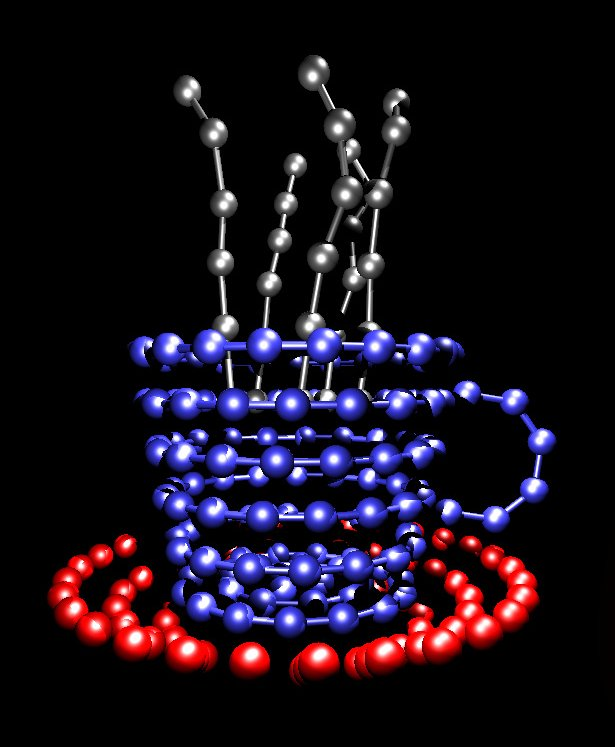
\includegraphics[width=5cm]{figures/logo}
  \end{center}
}
%\subject{}
\title{\es{} User's Guide}
%\author{}
%\date{\today}
\maketitle

\pdfbookmark{Contents}{toc}
\tableofcontents

\chapter{Introduction}
\label{chap:intro}

\todo{Make the following lists full text.}

\begin{itemize}
\item \es{} is a generic soft matter simulation packages
\item for molecular dynamics simulations in soft matter research
\item focussed on coarse-grained models
\item employs modern algorithms (Lattice-Boltzmann, DPD, P3M, \ldots)
\item written in C for maximal portability
\item Tcl-controlled
\item parallelized
\end{itemize}

\section{Guiding principles}
\label{sec:ideas}

(from paper: 2.1 Goals and principles)

\es
\begin{itemize}
\item does \emph{not} do the physics for you!
\item requires you to understand what you do (can not be used as a
  black box)
\item gives you maximal freedom (flexibility)
\item is extensible
\item integrates system setup, simulation and analysis, as this can't
  be strictly separated in soft matter simulations
\item has no predefined units
\item sets as few defaults as possible
\end{itemize}

\section{Algorithms contained in \es}

The following algorithms are implemented in \es{}:

\begin{itemize}
\item ensembles: NVE, NVT, NpT
\item charged systems:
  \begin{itemize}
  \item P3M for fully periodic systems
  \item ELC and MMM-family of algorithms for charged systems with
    non-periodic boundary conditions
  \item Maggs algorithm 
  \end{itemize}
\item Hydrodynamics:
  \begin{itemize}
  \item DPD (as a thermostat)
  \item Lattice-Boltzmann
  \end{itemize}
\end{itemize}

\section{Basic program structure}
\label{sec:structure}

(from paper: 2.2 Basic program structure)

\begin{itemize}
\item Control level: \texttt{Tcl}
\item ``Kernel'' written in \texttt{C}
\item This user's guide will focus on the control level
\end{itemize}

\section{On units}
\label{sec:units}
\index{units}
\index{length unit}
\index{time unit}
\index{energy unit}
\index{physical units}

What is probably one of the most confusing subjects for beginners of
\es is, that \es does not predefine any units.  While most MD programs
specify a set of units, like, for example, that all lengths are
measured in \AA ngstr\"om or nanometers, times are measured in nano- or
picoseconds and energies are measured in $\frac{kJ}{\mathrm{mol}}$,
\es does not do so.

Instead, the length-, time- and energy scales can be freely chosen by
the user.  A length of $1.0$ can mean a nanometer, an \AA ngstr\"om,
or a kilometer - depending on the physical system, that the user has
in mind when he writes his \es-script.  The user can choose the unit
system that suits the system best.

When creating particles that are intended to represent a specific type
of atoms, one will probably use a length scale of \AA ngstr\"om.  This
would mean, that \eg the parameter $\sigma$ of the Lennard-Jones
interaction between two atoms would be set to twice the van-der-Waals
radius of the atom in \AA ngstr\"om.  Alternatively, one could set
$\sigma$ to $2.0$ and measure all lengths in multiples of the
van-der-Waals radius.

The second choice to be made is the energy (and time-) scale.  One can
for example choose to set the Lennard-Jones parameter $\epsilon$ to
the energy in $\frac{kJ}{\mathrm{mol}}$.  Then all energies will be
measured in that unit.  Alternatively, one can choose to set it to
$1.0$ and measure everything in multiples of the van-der-Waals binding
energy.

As long as one remains within the same unit system throughout the
whole \es-script, there should be no problems.

\section{Requirements}
\label{sec:requirements}
\index{requirements}

The following libraries and tools are required to be able to compile
and use \es:

\begin{description}
\item[Tcl/Tk] \index{Tcl/Tk} \es{} requires the Toolkit Command
  Language Tcl/Tk \footnote{\url{http://www.tcl.tk/}} in the version
  8.3 or later.  Some example scripts will only work with Tcl 8.4. You
  do not only need the interpreter, but also the header files and
  libraries.  Depending on the operating system, these may come in
  separate development packages. If you want to use a graphical user
  interface (GUI) for your simulation scripts, you will also need Tk.
  
\item[FFTW] \index{FFTW} In addition, \es{} needs the FFTW library
  \footnote{\url{http://www.fftw.org/}} for Fourier transforms.
  ESPResSo can work with both the 2.1.x and 3.0.x series. Again, the
  header files are required.
  
\item[MPI] \index{MPI} Finally, if you want to use \es{} in parallel,
  you need a working MPI environment (version 1.2). Currently, the
  following MPI implementations are supported:
  \begin{itemize}
  \item LAM/MPI is the preferred variant
  \item MPICH, which seems to be considerably slower than LAM/MPI in
    our benchmarks.
  \item On AIX systems, \es{} can also use the native POE parallel
    environment.
  \item On DEC/Compaq/HP OSF/Tru64, \es{} can also use the native
    dmpirun MPI environment.
  \end{itemize}
\end{description}


\section{Syntax description}
\label{sec:syntax}


Throughout the user's guide, formal definitions of the syntax of
several Tcl-commands can be found. The following conventions are used
in these decriptions:
\begin{itemize}
\item Different \emph{variants} of a command are labelled \variant{1},
  \variant{2}, \ldots
\item Keywords and literals of the command that have to be typed
  exactly as given are written in \lit{typewriter} font.
\item If the command has variable arguments, they are set in
  \var{italic font}. The description following the syntax definition
  should contain a detailed explanation of the argument and its
  type.
\item \texttt{\alt{\var{alt1} \asep \var{alt2}}} specifies, that one
  of the alternatives \var{alt1} or \var{alt2} can be used.
\item \texttt{\opt{\var{argument}}} specifies, that the arugment
  \var{argument} is optional, \ie{} it can be omitted.
\item When an optional argument or a whole command is marked by a
  superscript label (\fmark{1}), this denotes that the argument can
  only be used, when the corresponding feature (see appendix
  \vref{chap:features}) specified in ``Required features'' is
  activated.
\end{itemize}


\minisec{Example}

\renewcommand{\variant}[1]{\par\rawvariant{#1}}
\begin{essyntaxbox}
  \variant{1} 
  constraint wall normal \var{n_x} \var{n_y} \var{n_z} 
  dist \var{d} type \var{id}
  
  \variant{2}
  constraint sphere center \var{c_x} \var{c_y} \var{c_z} 
  radius \var{rad} direction \var{direction} type \var{id} 
  
  \require{1}{%
    \variant{3}
    constraint rod center \var{c_x} \var{c_y} 
    lambda \var{lambda}
  } 
  
  \require{2,3}{%
    \variant{4}
    constraint ext_magn_field \var{f_x} \var{f_y} \var{f_z} 
  }

  \begin{features}
    \required{CONSTRAINTS}
    \required[1]{ELECTROSTATICS}
    \required[2]{ROTATION}
    \required[3]{DIPOLES}
  \end{features}

\end{essyntaxbox}
\renewcommand{\variant}[1]{\rawvariant{#1}}

%%% Local Variables: 
%%% mode: latex
%%% TeX-master: "ug"
%%% End: 


\chapter{First steps}
\label{chap:firststeps}

\section{Quick installation}

\index{configure}\index{make}

If you have the requirements (see section \vref{sec:requirements})
installed, in many cases, to compile \es{}, it is enough to execute
the following sequence of two steps in the directory where you have
unpacked the sources:
\begin{code}
configure
make
\end{code}

\todo{Mention minimal configuration without myconfig.h}
In some cases, \eg{} when \es{} needs to be compiled for several
different platforms or when different versions with different sets of
features are required, it might be useful to execute the commands not
in the source directory itself, but to start \texttt{configure} from
another directory (see section \vref{sec:builddir}). Furthermore, many
features of \es{} can be selectively turned on or off in the local
configuration header of \es{} (see section \vref{sec:myconfig}) before
starting the compilation with \texttt{make}.

The shell script \texttt{configure} prepares the source code for
compilation. It will determine how to use and where to find the
different libraries and tools required by the compilation process, and
it will test what compiler flags are to be used.  The script will find
out most of these things automatically.  If something is missing, it
will complain and give hints how to solve the problem.  The
configuration process can be controlled with the help of a number of
options that are explained in section \vref{sec:configure}.

The command \texttt{make} will compile the source code. Depending on
the options passed to the program, \texttt{make} can also be used for
a number of other things:
\begin{itemize}
\item It can install and uninstall the program to some other
  directories. However, normally it is not necessary to actually
  \textit{install} \es{} to run it.
\item It can test the \es{} program for correctness.
\item It can build the documentation.
\end{itemize}
The details of the usage of \texttt{make} are described in section
\vref{sec:make}.

When these steps have successfully completed, \es{} can be started
with the command (see section \vref{sec:run})
\begin{code}
Espresso
\end{code}

\section{Running \es}

\footnote{\url{http://www.tcl.tk/man/tcl8.5/tutorial/tcltutorial.html}}

\es{} is implemented as an extension to the Tcl script language. This means that you need to write a
script for any task you want to perform with \es. To learn about the Tcl script language and
especially the \es{} extensions, this chapter offers two tutorial scripts. The first will guide you
step by step through creating your first simulation script, while the second script is a well
documented example simulation script. Since the latter is slightly more complex and uses more
advanced features of \es{}, we recommend to work through both scripts in the presented order.

\section{Creating the first simulation script}

This section introduces some of the features of \es\ by
constructing step by step a simulation script for a simple salt crystal.
We cannot give a full Tcl tutorial here; however, most of the constructs
should be self--explanatory. We also assume that the reader is familiar with the
basic concepts of a MD simulation here. The code pieces can be copied step by
step into a file, which then can be run using \verb|Espresso <file>| from the
\es source directory.

Our script starts with setting up the initial configuration.  Most conveniently,
one would like to specify the density and the number of particles of the system
as parameters:
\begin{tclcode}
set n_part 200; set density 0.7
set box_l [expr pow($n_part/$density,1./3.)]
\end{tclcode}
These variables do not change anything in the simulation engine, but are just
standard Tcl variables; they are used to increase the readability and
flexibility of the script. The box length is not a parameter of this simulation;
it is calculated from the number of particles and the system density. This
allows to change the parameters later easily, e.~g.\ to simulate a bigger
system.

The parameters of the simulation engine are modified by the \verb|setmd|
command. For example
\begin{tclcode}
setmd box_l $box_l $box_l $box_l
setmd periodic 1 1 1
\end{tclcode}
defines a cubic simulation box of size \verb|box_l|, and periodic boundary
conditions in all spatial dimensions. We now fill this simulation box with
particles
\begin{tclcode}
set q 1; set type 0
for {set i 0} { $i < $n_part } {incr i} {
  set posx [expr $box_l*[t_random]]
  set posy [expr $box_l*[t_random]]
  set posz [expr $box_l*[t_random]]
  set q [expr -$q]; set type [expr 1-$type]
  part $i pos $posx $posy $posz q $q type $type 
}
\end{tclcode}
This loop adds \verb|n_part| particles at random positions, one by one.  In this
construct, only two commands are not standard Tcl commands: the random
number generator \verb|t_random| and the \verb|part| command, which is used to
specify particle properties, here the position, the charge \verb|q| and the
type. In \es\ the particle type is just an integer number which allows to group
particles; it does not imply any physical parameters. Here we use it to tag the
charges: positive charges have type 0, negative charges have type 1.

Now we define the ensemble that we will be simulating. This is done using the
\verb|thermostat| command. We also set some integration scheme parameters:
\begin{tclcode}
setmd time_step 0.01; setmd skin 0.4
set temp 1; set gamma 1
thermostat langevin $temp $gamma
\end{tclcode}
This switches on the Langevin thermostat for the NVT ensemble, with temperature
\verb|temp| and friction \verb|gamma|. The skin depth \verb|skin| is a parameter
for the link--cell system which tunes its performance, but cannot be discussed
here.

Before we can really start the simulation, we have to specify the
interactions between our particles.  We use a simple, purely repulsive
Lennard-Jones interaction to model the hard core repulsion
\citep{grest86a}, and the charges interact via the Coulomb potential:
\begin{tclcode}
set sig 1.0; set cut   [expr 1.12246*$sig]
set eps 1.0; set shift [expr 0.25*$eps]
inter 0 0 lennard-jones $eps $sig $cut $shift 0
inter 1 0 lennard-jones $eps $sig $cut $shift 0
inter 1 1 lennard-jones $eps $sig $cut $shift 0
inter coulomb 10.0 p3m tunev2 accuracy 1e-3 mesh 32
\end{tclcode}
The first three \verb|inter| commands instruct \es\ to use the same purely
repulsive Lennard--Jones potential for the interaction between all combinations
of the two particle types 0 and 1; by using different parameters for different
combinations, one could simulate differently sized particles.  The last line sets
the Bjerrum length to the value 10, and then
instructs \es\ to use P$^3$M for the Coulombic interaction and to try to find
suitable parameters for an rms force error below $10^{-3}$, with a fixed mesh
size of 32. The mesh is fixed here to speed up the tuning; for a real
simulation, one will also tune this parameter.

If we want to calculate the temperature of our system from the kinetic energy,
we need to know the number of the degrees of freedom of the particles.
In \es\ these are usually 3 translational plus 3 rotational degrees of freedom
(if ROTATION is compiled into the code). You can get this number
in the following way \footnote{Note: there also exists a predefined tcl function {\it degrees_of_freedom} which does the same.}:

\begin{tclcode}
   if { [regexp "ROTATION" [code_info]] } { 
     set deg_free 6
   } else { set deg_free 3 }
\end{tclcode}

Now we can integrate the system:
\begin{tclcode}
set integ_steps 200
for {set i 0} { $i < 20 } { incr i} {
  set temp [expr [analyze energy kinetic]/($deg_free/2.0)*$n_part)]
  puts "t=[setmd time] E=[analyze energy total], T=$temp"
  integrate $integ_steps 
}
\end{tclcode}
This code block is the primary simulation loop and runs
$20\times$\verb|integ_steps| MD steps. Every \verb|integ_steps| time steps, the
potential, electrostatic and kinetic energies are printed out (the latter one as
temperature). However, the simulation will crash: \es\ complains about particle
coordinates being out of range. The reason for this is simple: Due to the
initial random setup, the overlap energy is around a million kT, which we first
have to remove from the system. In \es, this is can be accelerated by capping
the forces, i.~e.\ modifying the Lennard--Jones force such that it is constant
below a certain distance. Before the integration loop, we therefore insert this
equilibration loop:
\begin{tclcode}
for {set cap 20} {$cap < 200} {incr cap 20} {
  puts "t=[setmd time] E=[analyze energy total]"
  inter ljforcecap $cap; integrate $integ_steps 
}
inter ljforcecap 0
\end{tclcode}
This loop integrates the system with a force cap of initially 20 and finally
200.  The last command switches the force cap off again. With this
equilibration, the simulation script runs fine.

However, it takes some time to simulate the system, and one will probably like
to write out simulation data to configuration files, for later analysis. For
this purpose \es\ has commands to write simulation data to a Tcl stream
in an easily parsable form.  We add the following lines at end of integration
loop to write the configuration files ``config\_0'' through ``config\_19'':
\begin{tclcode}
set f [open "config_$i" "w"]
blockfile $f write tclvariable {box_l density}
blockfile $f write variable box_l
blockfile $f write particles {id pos type}
close $f
\end{tclcode}
The created files ``config\_...'' are human--readable and look like
\begin{tclcode}
{tclvariable
        {box_l 10}
        {density 0.7}
}
{variable  {box_l 10.0 10.0 10.0} }
{particles {id pos type}
        {0 3.51770181433 4.3208975936 5.30529948918 0}
        {1 3.93145531704 6.58506447035 6.95045147034 1}
        ...
}
\end{tclcode}
As you can see, such a \emph{blockfile} consists of several Tcl lists,
which are called \emph{blocks}, and can store any data available from the
simulation. Reading a configuration is done by the following simple script:
\begin{tclcode}
set f [open $filename "r"]
while { [blockfile $f read auto] != "eof" } {}
close $f
\end{tclcode}
The \verb|blockfile read auto| commands will set the Tcl variables \verb|box_l|
and \verb|density| to the values specified in the file when encountering the
\verb|tclvariable| block, and set the box dimensions for the simulation when
encountering the \verb|variable| block. The particle positions and types of all
216 particles are restored when the \verb|particles| block is read. Note that it
is important to have the box dimensions set before reading the particles, to
avoid problems with the periodic boundary conditions.

\begin{figure}[tb]
  \centering
  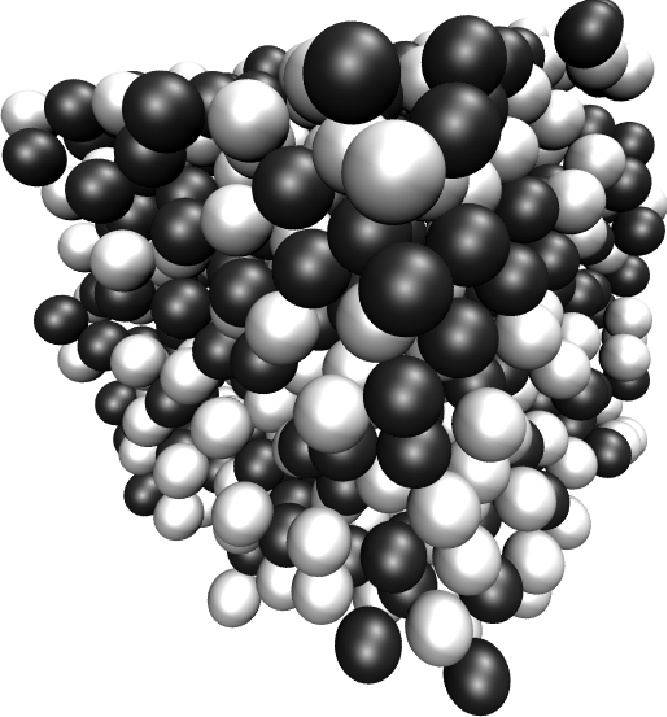
\includegraphics[width=0.4\textwidth]{figures/salt.png}
  \caption{VMD Snapshot of the salt system}
  \label{fig:snapshot}
\end{figure}

With these configurations, we can now investigate the system. As an example, we
will create a second script which calculates the averaged radial distribution
functions $g_{++}(r)$ and $g_{+-}(r)$. The radial distribution function for a
the current configuration can be obtained using the \verb|analyze| command:
\begin{tclcode}
set rdf [analyze rdf 0 1 0.9 [expr $box_l/2] 100]
set rlist ""
set rdflist ""
foreach value [lindex $rdf 1] {
  lappend rlist   [lindex $value 0]
  lappend rdflist [lindex $value 1] 
}
\end{tclcode}
The shown \verb|analyze rdf| command returns the distribution function of
particles of type 1 around particles of type 0 (i.~e.\ of opposite charges) for
radii between $0.9$ and half the box length, subdivided into $100$ bins.
Changing the first two parameters to either ``0 0'' or ``1 1'' allows to
determine the distribution for equal charges. The result is a list of $r$ and
$g(r)$ pairs, which the following foreach loop divides up onto two lists
\verb|rlist| and \verb|rdflist|.

To average over a set of configurations, we put the two last code snippets into
a loop like this:
\begin{tclcode}
set cnt 0
for {set i 0} {$i < 100} {incr i} { lappend avg_rdf 0}
foreach filename $argv {
  set f [open $filename "r"]
  while { [blockfile $f read auto] != "eof" } {}
  close $f
  set rdf [analyze rdf 0 1 0.9 [expr $box_l/2] 100]
  set rlist ""
  set rdflist ""
  foreach value [lindex $rdf 1] {
     lappend rlist   [lindex $value 0]
     lappend rdflist [lindex $value 1] }
  set avg_rdf [vecadd $avg_rdf $rdflist]
  incr cnt 
}
set avg_rdf [vecscale [expr 1.0/$cnt] $avg_rdf]
\end{tclcode}
Initially, the sum of all $g(r)$, which is stored in \verb|avg_rdf|, is set to
0.  Then the loops over all configurations given by \verb|argv|, calculates
$g(r)$ for each configuration and adds up all the $g(r)$ in \verb|avg_rdf|.
Finally, this sum is normalized by dividing by the number of
configurations. Note the ``1.0/\$cnt''; this is necessary, since ``1/\$cnt'' is
interpreted as an integer division, which results in 0 for $\text{cnt}>1$.
\verb|argv| is a predefined variable: it contains all the command line
parameters. Therefore this script should be called like
\begin{code}
Espresso \var{script} [\var{config}... ]
\end{code}

\begin{figure}[tb]
  \centering
  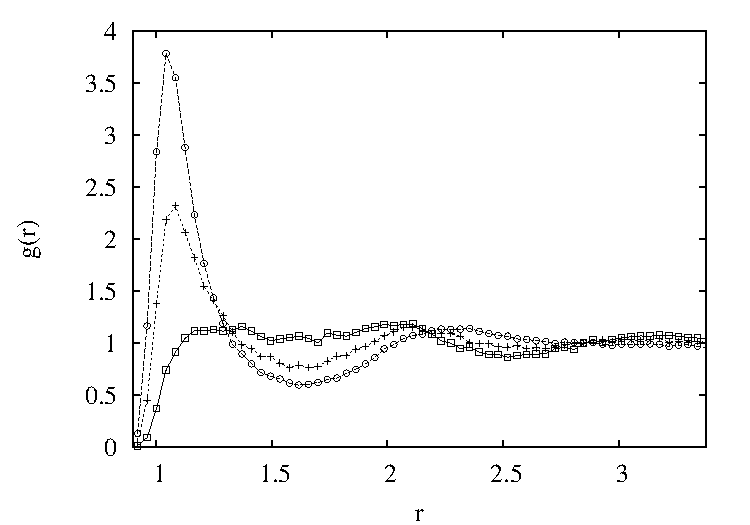
\includegraphics[width=0.7\textwidth]{figures/nacl-rdf.pdf}
  \caption{Radial distribution functions $g_{++}(r)$ between equal charges
    (rectangles) and $g_{+-}(r)$ for opposite charges (circles). The plus
    symbols denote $g(r)$ for an uncharged system.}
  \label{fig:rdf}
\end{figure}

The printing of the calculated radial distribution functions is simple. Add to the end of the
previous snippet the following lines:
\begin{tclcode}
set plot [open "rdf.data" "w"]
puts $plot "\# r rdf(r)"
foreach r $rlist rdf $avg_rdf { puts $plot "$r $rdf" }
close $plot
\end{tclcode}
This instructs the Tcl interpreter to write the \verb|avg_rdf| to the file \verb|rdf.data| in
gnuplot--compatible format. Fig.~\ref{fig:rdf} shows the resulting radial distribution functions,
averaged over 100 configurations. In addition, the distribution for a neutral
system is given, which can be obtained from our simulation script by simply
removing the command \verb|inter coulomb ...| and therefore not turning on P$^3$M.

The code example given before is still quite simple, and the reader is
encouraged to try to extend the example a little bit, e.~g. by using differently
sized particle, or changing the interactions. If something does not work, \es\
will give comprehensive error messages, which should make it easy to identify
mistakes. For real simulations, the simulation scripts can extend over thousands
of lines of code and contain automated adaption of parameters or online
analysis, up to automatic generation of data plots.  Parameters can be changed
arbitrarily during the simulation process, as needed for e.~g.\ simulated
annealing. The possibility to perform non--standard simulations without the need
of modifications to the simulation core was one of the main reasons why we
decided to use a script language for controlling the simulation core.

\section{\texttt{tutorial.tcl}}

In the directory \texttt{samples/} of the es{} sources, you will find
a well documented simulation script \texttt{tutorial.tcl}, which takes
you step by step through a slightly more complicated simulation of a
polyelectrolyte system. The basic structure of the script is however
the same as in the previous example and probably the same as the
structure of most \es{} simulation scripts.

Initially, some parameters and global variables are set, the
interactions are initialized, and particles are added. For this, the
script makes use of the \verb|polymer| command, which provides a
faster way to set up chain molecules.

The actual simulation falls apart again into two loops, the warmup
loop with increasing force capping, and the final simulation loop.
Note that the electrostatic interaction is only activated after
equilibrating the excluded volume interactions, which speeds up the
warmup phase. However, depending on the problem, this splitted warmup
may not be possible due to physical restrictions. \es{} cannot detect
these mistakes and it is your responsibility to find simulation
procedure suitable to your specific problem.

%%% Local Variables: 
%%% mode: latex
%%% TeX-master: "ug"
%%% End: 

\chapter{Compiling and installing \es}
\label{chap:install}
\index{Installation|textbf}

\begin{itemize}
\item Compiling \es{} is a necessary evil
\item Features can be compiled in or not
\item For maximal efficiency, compile in only the features that you
  use
\item \es{} can be obtained from the \es{} home page
  \footnote{\url{http://www.espresso.mpg.de}}.
\item If you are looking for the \es binary or the object files, read
  \vref{sec:builddir}
\item other than in most packages, \es will probably not be installed,
  or it will only be installed locally. Refer to \vref{sec:installdir}
  for details.
\end{itemize}

\section{Source and build directories}
\label{sec:builddir}
\index{build directory} \index{source directory}

Usually, when a program is compiled, the resulting binary files are
put into the same directory as the sources of the program. In \es, the
\emph{source directory} that contains all the source files is
completely separated from the \emph{build directory} where the files
created by the build process are put. As the source directory is not
modified during the compilation process, it is possible to compile more
than one binary versions of \es from a single set of source files.

The location of the build directory is determined when
\texttt{configure} is called.  Depending on whether it is called from
the source directory where it resides, or from some other directory,
the build system will act different.

When \texttt{configure} is called from another current working
directory than the source directory, this directory will become the
\emph{build directory}.  All files will be generated below the build
directory.  This way, you can make as many builds of \es as you like,
each build having different compiler flags and built-in features, and
for as many platforms as you want.  All further commands concerning
compiling and running \es{} have to be called from this directory,
instead of from the source directory.

When \texttt{configure} is called from the source directory where the
script resides, the \es build system has limited built-in capabilities
to handle different computer hardware.  A new subdirectory is created
in the source directory and \texttt{configure} is recursively called
from this directory, making the subdirectory the build directory.  The
directory is called \texttt{obj-}\textit{platform}\texttt{/}, where
\textit{platform} is an automatically determined descriptor of the CPU
type where the script was started, \eg
\mbox{\texttt{obj-Athlon\_64-pc-linux}}.  Note that this heuristic
will work in many cases, but it may not always work as intended.  When
you notice any problems, you can always call \texttt{configure} from
another directory.

In this case it is also possible to run the commands \texttt{make} and
\texttt{Espresso} directly in the source directory.  Furthermore, the
option \texttt{--enable-chooser} will be set in the recursive call of
\texttt{configure} that activates the automatic binary chooser (see
section \vref{sec:installdir}).

\paragraph{Example}
When the source directory is \texttt{\$srcdir} (\ie{} the files where
unpacked to this directory), then the build directory can be set to
\texttt{\$builddir} by calling the \texttt{configure}-script from
there:
\begin{code}
cd $builddir
$srcdir/configure
make
Espresso
\end{code}

\section{\texttt{myconfig.h}: Activating and deactivating features}
\label{sec:myconfig}

\index{features} \index{myconfig.h} \index{configuration header} \es
has a large number of features that can be compiled into the binary.
However, it is not recommended to actually compile in all possible
features, as this will negatively affect \es's performance.  Instead,
compile in only the features that are actually required.  For the
developers, it is also possible to turn on or off a number of
debugging messages.  The features and debug messages can be controlled
via a configuration header file that contains C-preprocessor
declarations. Appendix \vref{chap:features} lists and describes all
available features.  When no configuration header is provided by the
user, a default header will be used that turns on the default
features.  The file \texttt{myconfig-sample.h} in the source directory
contains a list of all possible features that can be copied into your
own configuration file.

When you distinguish between the build and the source directory (see
\vref{sec:builddir}), the configuration header can be put in either of
these. Note, however, that when a configuration header is found in
both directories, the one in the build directory will be used.  For an
example how this can be employed, see section \ref{sec:builddir}.

By default, the configuration header is called \texttt{myconfig.h}.
The name of the configuration header can be changed either when the
\texttt{configure}-script is called with the option
\mbox{\texttt{--with-myconfig}} (see section \vref{sec:configure}), or
when \texttt{make} is called with the setting
\mbox{\texttt{myconfig=}\textit{myconfig\_header}} (see section
\vref{sec:make}).

The configuration header can be used to compile different binary
versions of \es with a different set of features from the same source
directory.  Suppose that you have a source directory \texttt{\$srcdir}
and two build directories \texttt{\$builddir1} and
\texttt{\$builddir2} that contain different configuration headers:

\begin{itemize}
\item \texttt{\$builddir1/myconfig.h}:
\begin{code}
#define ELECTROSTATICS
#define LENNARD-JONES
\end{code}

\item \texttt{\$builddir2/myconfig.h}:
\begin{code}
#define LJCOS
\end{code}
\end{itemize}

\noindent Then you can simply compile two different versions of \es via
\begin{code}
cd $builddir1
$srcdir/configure
make

cd $builddir2
$srcdir/configure
make
\end{code}


\section{Running \texttt{configure}}
\label{sec:configure}

% Description of basic options: --prefix, --exec-prefix, CPPFLAGS,
% CFLAGS, LDFLAGS

\index{configure} The shell script \texttt{configure} collects all the
information required by the compilation process. It will determine how
to use and where to find the different libraries and tools required by
the compilation process, and it will test what compiler flags are to
be used.  The script will find out most of these things automatically.
If something is missing, it will complain and give hints how to solve
the problem.  The generic syntax of calling the \texttt{configure}
script is:
\begin{code}
configure [\var{options} ...] [\var{variable}=\var{value} ...]
\end{code}

\noindent Note that in the \es build system, the files generated by
the configuration and compilation process are not placed next to the
source files, but into a separate \emph{build directory} instead.
Refer to section \vref{sec:builddir} for details.

\index{configure options} The behaviour of \texttt{configure} can be
controlled by the means of command line options. In the following,
only those command line options that are specific to \es will be
explained.  For a complete list of options and explanations thereof,
call
\begin{code}
configure --help
\end{code}

\subsection{Options}

\begin{description}
\item [\texttt{--enable-chooser}] This option will enable the
  automatic binary chooser mechanism for \es (see section
  \vref{sec:installdir}).  This option will be automatically enabled,
  when the \texttt{configure} script is called from the source
  directory, otherwise it will be disabled. It is not recommended to
  set the option manually.
\item[\texttt{--enable-debug}] This option will enable compiler flags
  required for debugging the \es binary and is disabled by default.
\item[\texttt{--enable-profiling}] This option will enable compiler
  flags required for profiling the \es binary and is disabled by
  default.
\item[\texttt{--disable-processor-optimization}] This option will
  control whether \texttt{configure} will check for several
  optimization flags to be used by the compiler. This option is
  enabled by default.
\item[\texttt{--disable-xlc-qipa}] This option is only useful when the
  IBM C-compiler \texttt{xlc} is used and will control whether or not
  the compiler flag \texttt{-qipa} is used.  If you come upon problems
  when using the \es binary on IBM machines, try using
  \texttt{--disable-xlc-ipa}. The option is enabled by default.
\item[\texttt{--with-myconfig=MYCONFIG\_HEADER}] This option sets the
  name of the local configuration header (see \vref{sec:myconfig}). It
  defaults to ``\texttt{myconfig.h}''.
\item[\texttt{--with-mpi=MPI}/ \texttt{--without-mpi}] Sets the MPI
  implementation that should be used, or disables MPI. By default,
  \texttt{configure} will test automatically what MPI implementation
  is available. The following implementations are known:
  \begin{description}
  \item[\texttt{fake}, \texttt{no}] This will disable MPI
    completely. Equivalent to \mbox{\texttt{--without-mpi}}.
  \item[\texttt{lam}] Use the LAM/MPI environment
    (\url{http://www.lam-mpi.org/}).
  \item[\texttt{mpich}] Use the MPICH environment
    (\url{http://www-unix.mcs.anl.gov/mpi/mpich/}).
  \item[\texttt{poe}] Use the POE environment (IBM).
  \item[\texttt{dmpi}] Use the DMPI environment (Tru64).
  \item[\texttt{generic}] Use a generic MPI implementation. This will
    try to find an MPI compiler and an MPI runtime environment.
  \end{description}
\item[\texttt{--with-efence} / \texttt{--without-efence}] Whether or
  not to use the ``electric fence'' memory debugging library
  (\url{http://freshmeat.net/projects/efence/}). Efence is not used by
  default.
\item[\texttt{--with-tcl=TCL}] By default, \texttt{configure} will
  automatically determine which version of Tcl is used.  If the wrong
  version is chosen automatically, you can specify the name of the
  library with this option, \eg{} \texttt{tcl8.4}.
\item[\texttt{--with-tk=TK} / \texttt{--without-tk}] By default, the
  GUI toolkit Tk is not used by \es. This option can be used to
  activate Tk and to specify which Tk version to use, \eg{}
  \texttt{tk8.4}. If you only specify \texttt{--with-tk} and do not
  give a version number, \texttt{configure} will try to automatically
  deduce the right version.
\item[\texttt{--with-fftw=VERSION} / \texttt{--without-fftw}] This can
  be used to specify whether the FFTW library is to be used, and which
  version.  By default, version 3 will be used if it is found,
  otherwise version 2 is used.  Note that quite a number of central
  features of \es require FFTW.
\end{description}

\section{\texttt{make}: Compiling,  testing and installing \es}
\label{sec:make}

The command \texttt{make} is mainly used to compile the \es{} source
code, but it can do a number of other things. The generic syntax of
the \texttt{make} command is:
\begin{code}
make [\var{target}...] [\var{variable}=\var{value}]
\end{code}
When no target is given, the target \texttt{all} is used. The
following targets are available:
\begin{description}
\item[\texttt{all}] Compiles the complete \es source code. The
  variable \lit{myconf} can be used to specify the name of the
  configuration header to be used.
\item[\texttt{check}] Runs the testsuite. By default, all available
  tests will be run on 1, 2, 3, 4, 6, or 8 processors. Which tests are
  run can be controlled by means of the variable \texttt{tests}, which
  processor numbers are to be used can be controlled via the variable
  \texttt{processors}. Note that depending on your MPI installation,
  MPI jobs can only be run in the queueing system, so that \es{} will
  not run from the command line. In that case, you may not be able to
  run the testsuite, or you have to directly submit the testsuite script
  \verb!testsuite/test.sh! to the queueing system.\\
  \textbf{Example:} \verb!make check tests="madelung.tcl" processors="1 2"!\\
  will run the test \texttt{madlung.tcl} on one and two processors.
\item[\texttt{clean}] Deletes all files that were created during the
  compilation.
\item[\texttt{mostlyclean}] Deletes most files that were created
  during the compilation. Will keep for example the built doxygen
  documentation and the \es{} binary.
\item[\texttt{dist}] Creates a \texttt{.tar.gz}-file of the \es{}
  sources.  This will include all source files as they currently are
  in the source directory, \ie{} it will include local changes.  This
  is useful to give your version of \es{} to other people.
  The variable \texttt{extra} can be used to specify additional
  files and directories that are to be included in the archive
  file. \\
  \textbf{Example:} \verb!make dist extra="myconfig.h internal"!\\
  will create the archive file and include the file
  \texttt{myconfig.h} and the directory \texttt{internal} with all
  files and subdirectories.
\item[\texttt{install}] Install \es. The variables \texttt{prefix} and
  \texttt{exec-prefix} can be used to specify the installation
  directories, otherwise the defaults defined by the
  \texttt{configure} script are used. \texttt{prefix} sets the prefix
  where all \es files are to be installed, \texttt{exec-prefix} sets
  the prefix where the executable files are to be installed and is
  required only when there is an architecture-specific directory (\eg
  \texttt{/usr/local/bin64/}).  For the actual locations where the
  different files are installed, refer to section
  \vref{sec:installdir}.\\
  \textbf{Example:} \verb!make install prefix=/usr/local!\\
  will install all files below \texttt{/usr/local}.
\item[\texttt{uninstall}] Uninstalls \es{}, \ie{} removes all files
  that were installed during \texttt{make install}. The variables are
  identical to the variables of the \texttt{install}-target.
\end{description}

\subsection{Installation directories}
\label{sec:installdir}

\index{installation directory} Other than most software, \es is not
necessarily installed into the system, but can also be used directly
from the build directory.  The rest of this section is only
interesting if you plan to install \es.

Normally, the \es-binary \texttt{Espresso-bin} is installed in the
directory \texttt{\$prefix/libexec/} and a the wrapper script
\texttt{Espresso} in the directory \texttt{\$prefix/bin/} that handles
the MPI invocation.

When the \texttt{configure}-script is called from the source directory
or when the option \texttt{--enable-chooser} is given, an automatic
binary chooser is installed in the directory \texttt{\$prefix/bin/}
and the \es-binary and the MPI wrapper script are installed in an
architecture-specific subdirectory
\mbox{\texttt{\$exec-prefix/lib/espresso/obj-}\textit{platform}\texttt{/}}.
When called, the binary chooser will automatically call the MPI
wrapper script from the right subdirectory.

\section{Running \es}
\label{sec:run}

When \es is found in your path, it can be run via
\begin{code}
Espresso [\var{tcl\_script} [\var{N\_processors} [\var{args}]]]
\end{code}

\index{interactive mode} When \es{} is called without any arguments,
it is started in the interactive mode, where new commands can be
entered on the command line. When the name of a \textit{tcl\_script}
is given, the script is executed. \textit{N\_processors} is the number
of processors that are to be used. Any further arguments are passed to
the script. Note that depending on your MPI installation, MPI jobs can
only be run in the queueing system, so that \es will not run from
the command line.

% A number of wrapper scripts are used in running \es{}:
% \begin{itemize}
% \item The script \texttt{Espresso} in the source and build directory
%   will try to run the compiled version of \es. If it is called from
%   the source directory, it assumes that \es{} was also configured in
%   the source directory and will try to recursively start the script in
%   the corresponding \texttt{obj-PLATFORM} build directory. If it is
%   called in the build directory, it will start the \es-binary with the
%   right MPI implementation.
% \item The chooser script \texttt{Espresso} 
%   \begin{itemize}
%   \item installed when \verb!--enable-chooser! was given
%   \item installed to bindir
%   \item tries to run the correct version of the MPI-wrapper
%     \texttt{Espresso}
%   \end{itemize}
% \item The MPI-wrapper \texttt{Espresso}
%   \begin{itemize}
%   \item installed next to \es{} binary
%   \item starts the binary with the right MPI implementation
%   \end{itemize}
% \item The \es{} binary \texttt{Espresso-bin} can also be started
%   directly, however, it requires that the environment variable
%   \verb!ESPRESSO_SCRIPTS! is set to the directory where the scripts
%   are installed (usually \verb!$(prefix)/lib/espresso/scripts! or
%   \verb!$(prefix)/share/espresso/scripts!).
% \end{itemize}


%%% Local Variables: 
%%% mode: latex
%%% TeX-master: "ug"
%%% End: 

\chapter{Setting up the system}
\label{chap:setup}

\section{\texttt{setmd}: Setting global variables.}
\newescommand{setmd}

\begin{essyntax}
\variant{1} setmd \var{variable}
\variant{2} setmd \var{variable} \opt{\var{value}}+
\end{essyntax}
\todo{Explain '+' in intro.}

Variant \variant{1} returns the value of the \es global variable
\var{variable}, variant \variant{2} can be used to set the variable
\var{variable} to \var{value}. The following global variables can be
set:

%% List-environment for the description of the global variables
\newenvironment{globvar}{
  \begin{list}{}{
      \setlength{\rightmargin}{1em}
      \setlength{\leftmargin}{2em}
      \setlength{\partopsep}{0pt}
      \setlength{\topsep}{1ex}
      \setlength{\parsep}{0.5ex}
      \setlength{\listparindent}{-1em}
      \setlength{\labelwidth}{0.5em}
      \setlength{\labelsep}{0.5em}
      \renewcommand{\makelabel}[1]{%
        \index{##1@\texttt{##1} (global variable)|mainindex}%
        \index{global variables!\texttt{##1}|mainindex}%
        \texttt{##1}%
      }
    }
  }{
  \end{list}
}
\newcommand{\ro}{\emph{read-only}}

\todo{Better throw some out (\eg switches)?}
\todo{Missing: lattice_switch, dpd_tgamma, n_rigidbonds}
\todo{Which commands can be used to set the \emph{read-only}
  variables?}
\begin{globvar}
\item[box_l] (double[3]) Simulation box length.
  \todo{document what happens to the particles when \keyword{box_l} is
    changed!}
\item[cell_grid] (int[3], \ro) Dimension of the inner
  cell grid.
\item[cell_size] (double[3], \ro) Box-length of a cell.
\item[dpd_gamma] (double, \ro) Friction constant for the
  DPD thermostat.
\item[dpd_r_cut] (double, \ro) Cutoff for DPD thermostat.
\item[gamma] (double, \ro) Friction constant for the
  Langevin thermostat.
\item[integ_switch] (int, \ro) Internal switch which integrator to
  use.
\item[local_box_l] (int[3], \ro) Local simulation box length of the
  nodes.
\item[max_cut] (double, \ro) Maximal cutoff of real space
  interactions.
\item[max_num_cells] (int) Maximal number of cells for the link cell
  algorithm.  Reasonable values are between 125 and 1000, or for some
  problems (\var{n_total_particles} / \var{n_nodes}).
\item[max_part] (int, \ro) Maximal identity of a particle.
  \emph{This is in general not related to the number of particles!}
\item[max_range] (double, \ro) Maximal range of real space
  interactions: \var{max_cut} + \var{skin}.
\item[max_skin] (double, \ro) Maximal skin to be used for the link
  cell/verlet algorithm. This is the minimum of \var{cell_size} -
  \var{max_range}. \todo{???}
\item[min_num_cells] (int) \todo{???} Minimal number of cells for the
  link cell algorithm. Reasonable values range in $1e-6 N^2$ to $1e-7
  N^2$. In general just make sure that the Verlet lists are not
  incredibly large. By default the minimum is 0, but for the automatic
  P3M tuning it may be wise to larger values for high particle
  numbers.
\item[n_layers] (int, \ro) Number of layers in cell structure LAYERED
  (see section \vref{sec:cell-systems}).
\item[n_nodes] (int, \ro) Number of nodes.
\item[n_part] (int, \ro) Total number of particles.
\item[n_part_types] (int, \ro) Number of particle types that were
  used so far in the \keyword{inter} command (see chapter{tcl:inter}).
\item[node_grid] (int[3]) 3D node grid for real space domain
  decomposition (optional, if unset an optimal set is chosen
  automatically).
\item[nptiso_gamma0] (double, \ro)\todo{Docs missing.}
\item[nptiso_gammav] (double, \ro)\todo{Docs missing.}
\item[npt_p_ext] (double, \ro) Pressure for NPT simulations.
\item[npt_p_inst] (double) Pressure calculated during an
  NPT_isotropic integration.
\item[piston] (double, \ro) Mass off the box when using NPT_isotropic
  integrator.
\item[periodicity] (bool[3]) Specifies periodicity for the three
  directions. If the feature PARTIAL_PERIODIC is set, this variable
  can be set to (1,1,1) or (0,0,0) at the moment.  If not it is
  readonly and gives the default setting (1,1,1).\todo{Correct?}
\item[skin] (double) Skin for the Verlet list.
\item [temperature] (double, \ro) Temperature of the
  simulation.
\item[thermo_switch] (double, \ro) Internal variable which thermostat
  to use. 
\item[time] (double) The simulation time.
\item[time_step] (double) Time step for MD integration.
\item[timings] (int) Number of timing samples to take into account if
  set.\todo{???}
\item[transfer_rate] (int, \ro) Transfer rate for VMD connection. You
  can use this to transfer any integer value to the simulation from
  VMD.
\item[verlet_flag] (bool) Indicates whether the Verlet list will be
  rebuild. The program decides this normally automatically based on
  your actions on the data.
\item[verlet_reuse] (double) Average number of integration steps the
  verlet list has been re-used.
\end{globvar}

\section{\texttt{thermostat}: Setting up the thermostat}
\newescommand{thermostat}

\begin{essyntax}
  \variant{1} thermostat off
  \variant{2} theormstat \var{method} \opt{\var{parameter}}+
\end{essyntax}
\todo{Include docs from \texttt{thermostat.h}!}
Change thermostat settings.

\section{\texttt{nemd}: Setting up non-equilibrium MD}
\newescommand{nemd}

\begin{essyntax}
  \variant{1}nemd \var{method} \var{parameter} 
  \variant{2}nemd off
  \variant{3}nemd profile
  \variant{4}nemd viscosity
\end{essyntax}
\todo{Include docs from \texttt{nemd.h}!}
\todo{Put \texttt{nemd profile|viscosity} into \texttt{analyze}?}  
Use NEMD (Non Equilibrium Molecular Dynamics) to simulate a system
under shear.

\section{\texttt{cellsystem}: Setting up the cell system}
\label{sec:cell-systems}
\newescommand{cellsystem}

This section deals with the flexible particle data organization of
\es.  Due to different needs of different algorithms, \es is able to
change the organization of the particles in the computer memory,
according to the needs of the used algorithms. For details on the
internal organization, refer to section
\vref{sec:internal-particle-organization}.

\subsection{Domain decomposition}
\index{domain decomposition}
\begin{essyntax}
  cellsystem domain_decomposition \opt{-no_verlet_list}
\end{essyntax}
This selects the domain decomposition cell scheme, using Verlet lists
for the calculation of the interactions. If you specify
\keyword{-no_verlet_list}, only the domain decomposition is used, but
not the Verlet lists.

The domain decomposition cellsystem is the default system and suits
most applications with short ranged interactions. The particles are
divided up spatially into small compartments, the cells, such that the
cell size is larger than the maximal interaction range. In this case
interactions only occur between particles in adjacent cells. Since the
interaction range should be much smaller than the total system size,
leaving out all interactions between non-adjacent cells can mean a
tremendous speed-up. Moreover, since for constant interaction range,
the number of particles in a cell depends only on the density. The
number of interactions is therefore of the order N instead of order
$N^2$ if one has to calculate all pair interactions.

\subsection{N-squared}
\begin{essyntax}
  cellsystem nsquare 
\end{essyntax}
This selects the very primitive nsquared cellsystem, which calculates
the interactions for all particle pairs. Therefore it loops over all
particles, giving an unfavorable computation time scaling of $N^2$.
However, algorithms like MMM1D or the plain Coulomb interaction in the
cell model require the calculation of all pair interactions.

In a multiple processor environment, the nsquared cellsystem uses a
simple particle balancing scheme to have a nearly equal number of
particles per CPU, \ie $n$ nodes have $m$ particles, and $p-n$ nodes
have $m+1$ particles, such that $n*m+(p-n)*(m+1)=N$, the total number
of particles. Therefore the computational load should be balanced
fairly equal among the nodes, with one exception: This code always
uses one CPU for the interaction between two different nodes. For an
odd number of nodes, this is fine, because the total number of
interactions to calculate is a multiple of the number of nodes, but
for an even number of nodes, for each of the $p-1$ communication
rounds, one processor is idle.

E.g. for 2 processors, there are 3 interactions: 0-0, 1-1, 0-1.
Naturally, 0-0 and 1-1 are treated by processor 0 and 1, respectively.
But the 0-1 interaction is treated by node 1 alone, so the workload
for this node is twice as high. For 3 processors, the interactions are
0-0, 1-1, 2-2, 0-1, 1-2, 0-2. Of these interactions, node 0 treats 0-0
and 0-2, node 1 treats 1-1 and 0-1, and node 2 treats 2-2 and 1-2.

Therefore it is highly recommended that you use nsquared only with an
odd number of nodes, if with multiple processors at all. 

\subsection{Layered cell system}
\begin{essyntax}
  cellsystem layered \var{n_layers}
\end{essyntax}

This selects the layered cell system, which is specifically designed
for the needs of the MMM2D algorithm. Basically it consists of a
nsquared algorithm in x and y, but a domain decomposition along z, i.
e. the system is cut into equally sized layers along the z axis. The
current implementation allows for the cpus to align only along the z
axis, therefore the processor grid has to have the form 1x1xN.
However, each processor may be responsible for several layers, which
is determined by \var{n\_layers}, i. e. the system is split into
N*\var{n\_layers} layers along the z axis. Since in x and y direction
there are no processor boundaries, the implementation is basically
just a stripped down version of the domain decomposition cellsystem.

%%% Local Variables: 
%%% mode: latex
%%% TeX-master: "ug"
%%% End: 

\chapter{Running the simulation}
\label{chap:run}

\section{\texttt{integrate}: Running the simulation}
\eslabel{integrate}

\begin{essyntax}
  \variant{1} integrate \var{steps}
  \variant{2} integrate set \var{method} \opt{\var{parameter}}+
\end{essyntax}

\todo{Docs missing!}
\todo{Which integrators do exist?}

\section{\texttt{change_volume}: Changing the box volume}
\eslabel[change-volume]{change_volume}

\begin{essyntax}
  \variant{1} change_volume \var{V_new} 
  \variant{2} change_volume \var{L_new} \alt{x \asep y \asep z \asep xyz}
\end{essyntax}
Changes the volume of either a cubic simulation box to the new volume
\var{V_new} or its given x-/y-/z-/xyz-extension to the new box-length
\var{L_new}, and isotropically adjusts the particles coordinates as
well. The function returns the new volume of the deformed simulation
box.

\section{Stopping particles}
\eslabel{stopParticles}
\eslabel[stop-particles]{stop_particles}

\begin{essyntax}
  \variant{1} stopParticles
  \variant{2} stop_particles
\end{essyntax}
Halts all particles in the current simulation, setting their
velocities and forces to zero. Variant \variant{2} does not provide
feedback on the execution status.

\section{\texttt{velocities}: Setting the velocities}
\eslabel{velocities}
\begin{essyntax}
  velocities \var{v_max} 
  \opt{start \var{part_id}} 
  \opt{count \var{N_T}}
\end{essyntax}
Sets the velocities of the particles with particle ID (see The part
command) between \var{part_id} and \var{part_id}+\var{N_T}
(defaults to '0' \& '[setmd npart]-\var{part_id}') to a random vector
with length in [-vmax,vmax], and returns the absolute value of the
total velocity assigned.

\section{\texttt{invalidate_system}}
\eslabel[invalidate-system]{invalidate_system}
\begin{essyntax}
  invalidate_system
\end{essyntax}
\todo{Documentation not up to date!}

Forces a system re-init which, among others, causes the integrator to
also update the forces at its beginning (instead of re-using the
values from the previous integration step).  This is particularly
necessary to ensure continuity after setting a checkpoint:
\texttt{integrate} - \texttt{set_checkpoint} - \texttt{integrate} has
only one call to \todo{???}???, while \texttt{read_checkpoint} -
\texttt{integrate} has two at the beginning of the 2nd integrate
(because loading a new system from disk typically requires
re-initializing the system), and since ??? also uses the thermostat
which in turn draws random numbers, the two situations do not end up
at the same segment of the random number sequence, all random events
will therefore slightly differ.  To prevent this, simply include a
call to invalidate_system upon setting the checkpoint (this is being
done automatically if using tcl_checkpoint_set and
tcl_checkpoint_read beginning with v1.1 of \es{}), because in that
case both scenarios will call ??? twice at the beginning of the second
integration phase thus having their random number sequences in total
sync. The C implementation is invalidate_system.



%%% Local Variables: 
%%% mode: latex
%%% TeX-master: "ug"
%%% End: 

\chapter{Analysis}
\label{chap:analysis}


%%% Local Variables: 
%%% mode: latex
%%% TeX-master: "ug"
%%% End: 

\chapter{Auxilliary commands}
\label{chap:aux}

\section{Writing VTF files}
%\quickrefheading{Handling of VTF files}

There are two commands in \es{} that support writing files in the VMD
formats VTF, VSF and VCF.\footnote{A description of the format and a
  plugin to read the format in VMD is found in the subdirectory
  \texttt{vmdplugin/} of the \es{} source directory.} The commands can
be used to write the structure (\texttt{writevsf}) and coordinates
(\texttt{writevcf}) of the system to a single trajectory file (usually
with the extension \texttt{.vtf}), or to separate files (extensions
\texttt{.vsf} and \texttt{.vtf}).

\subsection{\texttt{writevsf}}

\tclcommand{writevsf}
{\var{file} [<short|verbose>] [<\var{radii}|auto>] [typedesc \var{typedesc}]}

Writes a structure block describing the system's structure to
\var{file}. The atom ids used in the file are identical to \es's
particle ids.  This makes it easy to write additional structure lines
to the file, e.g. to specify the \texttt{resname} of particle
compounds, like chains.  The output of this file can be used in a
standalone VSF file, or at the beginning of a trajectory VTF file that
contains a trajectory of a whole simulation.

\begin{tcloptions}
  \option{<short|verbose>}
  Specify, whether the output is in a human-readable, but somewhat
  longer format (\keyword{verbose}), or in a more compact form
  (\keyword{short}). The default is \keyword{verbose}.
  
  \option{<radius \var{radii}|auto>}
  Specify the VDW radii of the atoms. \var{radii} is either
  \keyword{auto}, or a Tcl-list describing the radii of the different
  particle types. When the keyword \keyword{auto} is used and a
  Lennard-Jones interaction between two particles of the given type is
  defined, the radius is set to be $\frac{\sigma_{LJ}}{2}$ plus the LJ
  shift.  Otherwise, the radius $0.5$ is substituted. The default is
  \keyword{auto}.
  
  Example: \verb!writevsf "show.tcl" radius {{0 2.0} {1 auto} {2 1.0}}!
  
  \option{typedesc \var{typedesc}}
  \var{typedesc} is a Tcl-list giving additional VTF atom-keywords to
  specify additional VMD characteristics of the atoms of the given type.
  If no description is given for a certain particle type, it defaults to
  \texttt{segid \textit{n}}, where \textit{n} is the type id.

  Example: \verb!writevsf "show.tcl" typedesc {{0 "segid colloid"} {1 "segid pe"}}!
\end{tcloptions}


\subsection{\texttt{writevcf}}
\tclcommand{writevcf}
{\var{file} [<short|verbose>] [<folded|absolute>]}

Writes a coordinate (or timestep) block that contains all coordinates
of the system's particles to \var{file}.

\begin{tcloptions}
  \option{<short|verbose>} Specify, whether the output is in a
  human-readable, but somewhat longer format (\keyword{verbose}), or
  in a more compact form (\keyword{short}). The default is
  \keyword{verbose}.

  \option{<folded|absolute>} Specify whether the particle positions
  are written in absolute coordinates (\keyword{absolute}) or folded
  into the central image of a periodic system (\keyword{folded}). The
  default is \keyword{absolute}.

  \option{<pids \var{pids}|all>} Specify the coordinates of which particles
  should be written. If \keyword{all} is used, all coordinates will be
  written (in the ordered timestep format). Otherwise, \var{pids} has
  to be a Tcl-list specifying the pids of the particles. The default
  is \keyword{all}.
  
  Example: \verb!pids {0 23 42}!

\end{tcloptions}


%%% Local Variables: 
%%% mode: latex
%%% TeX-master: "ug"
%%% End: 

\chapter{Under the hood}
\label{chap:underhood}

(new)

\begin{itemize}
\item Implementation issues that are interesting for the user
\item Main loop in pseudo code (for comparison)
\item from doxygen: ``Cell systems'' 
\end{itemize}

%%% Local Variables: 
%%% mode: latex
%%% TeX-master: "ug"
%%% End: 

\chapter{Getting involved}
\label{chap:devel}

\begin{itemize}
\item What to do when you want to become involved
\item How to submit a bug report
\item Reference to developer's guide
\end{itemize}

%%% Local Variables: 
%%% mode: latex
%%% TeX-master: "ug"
%%% End: 


\appendix
\chapter{\es{} quick reference}
\label{chap:quickref}

\index{quick reference of Tcl-commands}
%\input{ug.qrf}
%\listofcommands

%%% Local Variables: 
%%% mode: latex
%%% TeX-master: "ug"
%%% End: 

\chapter{Features}
\label{sec:features}
\index{features|textbf}

\newcommand{\feature}[1]{\texttt{\textbf{#1}}}

This chapter describes the features that can be activated in \es. Even
if possible, it is not recommended to activate all features, because
this will negatively effect \es's performance.

Features can be activated in the configuration header (see section
\vref{sec:myconfig}). Too activate \texttt{FEATURE}, add the following
line to the header file:
\begin{verbatim}
#define FEATURE
\end{verbatim}

\subsection{General features}
\begin{itemize}
\item \feature{PARTIAL\_PERIODIC} By default, all coordinates in \es{} are periodic. With
  \texttt{PARTIAL\_PERIODIC} turned on, the \es{} global variable \texttt{periodic} (see
  Sec.~\ref{sec:globalvar}) controls the periodicity of the individual coordinates. Note that this
  slows the integrator down by around $10-30\%$.
\item \feature{ELECTROSTATICS} This switches on the various electrostatics algorithms, such as
  the Ewald summation. See Sec.~\ref{sec:electrostatics} for details on this algorithms.
\item \feature{ROTATION} Switch on rotational degrees of freedom for the particles, as well as
  the corresponding quaternion integrator. See Sec.~\ref{sec:rotation} for details.
\item \feature{DIPOLES} This activates the dipole support in P$^3$M. Currently, a mixing of
  dipoles and charges is not possible, i.~e. all particles have to have charge $q=0$.
  Requires \texttt{ELECTROSTATICS} and \texttt{ROTATION}.
\item \feature{EXTERNAL\_FORCES} Allows to define an arbitrary constant force for each particle
  individually. Also allows to fix individual coordinates of particles, e.~g. keep them at a fixed
  position or within a plane.
\item \feature{CONSTRAINTS} Turns on various spatial constraints such as spherical compartments
  or walls. This constraints interact with the particles through regular short ranged potentials
  such as the Lennard--Jones potential. See Sec.~\ref{sec:constraints} for possible constraint
  forms.
\item \feature{MASS} Allows particles to have individual masses. Note that some analyzation
  procedures have not yet been adapted to take the masses into account correctly.
\item \feature{EXCLUSIONS} Allows to exclude specific short ranged interactions within
  molecules, which is necessary for some atomistic models.
\item \feature{COMFORCE}
\item \feature{COMFIXED}
\item \feature{MOLFORCES}
\item \feature{BOND\_CONSTRAINT} Turns on the RATTLE integrator which allows for fixed lengths
  bonds between particles.
\end{itemize}

In addition, there are switches that enable additional features in the integrator:
\begin{itemize}
\item \feature{NEMD} Enables the non-equilbrium (shear) MD support (see Sec.~\ref{sec:NEMD}).
\item \feature{NPT} Enables an on--the--fly NPT integration scheme (see Sec.~\ref{sec:NPT}).
\item \feature{DPD} Enables the dissipative particle dynamics thermostat (see
  Sec.~\ref{sec:DPD}).
\item \feature{LB} Enables the lattice-Boltzmann fluid code (see Sec.~\ref{sec:LB}).
\end{itemize}

\subsection{Interactions}
The following switches turn on various short ranged interactions (see Sec.~\ref{sec:shortrange}):
\begin{itemize}
\item \feature{TABULATED} Enable support for user--defined interactions, e.~g. for atomistic
  simulations.
\item \feature{LENNARD\_JONES} Enable the Lennard--Jones potential.
\item \feature{LJ\_WARN\_WHEN\_CLOSE} This adds an additional check to the Lennard--Jones
  potential that prints a warning of particles come too close so that the simulation becomes
  unphysical.
\item \feature{MORSE} Enable the Morse potential.
\item \feature{LJCOS} Enable the Lennard--Jones potential with a cosine--tail.
\item \feature{LJCOS2}
\item \feature{BUCKINGHAM} Enable the Buckingham potential.
\item \feature{SOFT\_SPHERE} Enable the soft sphere potential.
\end{itemize}

If you want to use angle bonds, you currently need to choose the type
a priori (see section \vref{sec:angle}). This will change in the near
future to three independent angle potentials:
\begin{itemize}
\item \feature{BOND\_ANGLE\_HARMONIC}
\item \feature{BOND\_ANGLE\_COSINE}
\item \feature{BOND\_ANGLE\_COSSQUARE}
\end{itemize}

\subsection{Debug messages}
Finally, there are a number of flags for debugging. The most important one are
\begin{itemize}
\item \feature{ADDITIONAL\_CHECKS} Enables numerous additional checks which can detect
  inconsistencies especially in the cell systems. This checks are however too slow to be enabled in
  production runs.
\item \feature{MEM\_DEBUG} Enables an internal memory allocation checking system. This produces
  output for each allocation and freeing of a memory chunk, and therefore allows to track down
  memory leaks. This works by internally replacing \texttt{malloc}, \texttt{realloc} and
  \texttt{free}.
\end{itemize}

The following flags control the debug output of various sections of Espresso. You will however
understand the output very often only by looking directly at the code.
\begin{itemize}
\item \feature{COMM\_DEBUG} Output from the asynchronous communication code.
\item \feature{EVENT\_DEBUG} Notifications for event calls, i.~e. the \texttt{on\_?} functions
  in \texttt{initialize.c}. Useful if some module does not correctly respond to changes of e.~g.
  global variables.
\item \feature{INTEG\_DEBUG} Integrator output.
\item \feature{CELL\_DEBUG} Cellsystem output.
\item \feature{GHOST\_DEBUG} Cellsystem output specific to the handling of ghost cells and the
  ghost cell communication.
\item \feature{GHOST\_FORCE\_DEBUG}
\item \feature{VERLET\_DEBUG} Debugging of the Verlet list code of the domain decomposition cell
  system.
\item \feature{LATTICE\_DEBUG} Universal lattice structure debugging.
\item \feature{HALO\_DEBUG}
\item \feature{GRID\_DEBUG}
\item \feature{PARTICLE\_DEBUG} Output from the particle handling code.
\item \feature{P3M\_DEBUG}
\item \feature{ESR\_DEBUG} debugging of P$^3$Ms real space part.
\item \feature{ESK\_DEBUG} debugging of P$^3$Ms $k$--space part.
\item \feature{EWALD\_DEBUG}
\item \feature{FFT\_DEBUG} Output from the unified FFT code.
\item \feature{MAGGS\_DEBUG}
\item \feature{RANDOM\_DEBUG}
\item \feature{FORCE\_DEBUG} Output from the force calculation loops.
\item \feature{THERMO\_DEBUG} Output from the thermostats.
\item \feature{LJ\_DEBUG} Output from the Lennard--Jones code.
\item \feature{MORSE\_DEBUG} Output from the Morse code.
\item \feature{FENE\_DEBUG}
\item \feature{ONEPART\_DEBUG} Define to a number of a particle to obtain output on the forces
  calculated for this particle.
\item \feature{STAT\_DEBUG}
\item \feature{POLY\_DEBUG}
\item \feature{MOLFORCES\_DEBUG}
\item \feature{LB\_DEBUG} Output from the lattice--Boltzmann code.
\item \feature{ASYNC\_BARRIER} Introduce a barrier after each asynchronous command
  completion. Helps in detection of mismatching communication.
\item \feature{FORCE\_CORE} Causes \es{} to try to provoke a core dump when exiting
  unexpectedly.
\item \feature{MPI\_CORE} Causes \es{} to try this even with MPI errors.
\end{itemize}

%%% Local Variables: 
%%% mode: latex
%%% TeX-master: "ug"
%%% End: 


\chapter{The MMM family of algorithms}
\label{chap:mmm}

\chapter{Maggs algorithm}
\label{chap:maggs}

\printindex

\end{document}


%%% Local Variables: 
%%% mode: latex
%%% TeX-master: t
%%% End: 

%\listofcommands

%%% Local Variables: 
%%% mode: latex
%%% TeX-master: "ug"
%%% End: 

\chapter{Features}
\label{sec:features}
\index{features|textbf}

\newcommand{\feature}[1]{\texttt{\textbf{#1}}}

This chapter describes the features that can be activated in \es. Even
if possible, it is not recommended to activate all features, because
this will negatively effect \es's performance.

Features can be activated in the configuration header (see section
\vref{sec:myconfig}). Too activate \texttt{FEATURE}, add the following
line to the header file:
\begin{verbatim}
#define FEATURE
\end{verbatim}

\subsection{General features}
\begin{itemize}
\item \feature{PARTIAL\_PERIODIC} By default, all coordinates in \es{} are periodic. With
  \texttt{PARTIAL\_PERIODIC} turned on, the \es{} global variable \texttt{periodic} (see
  Sec.~\ref{sec:globalvar}) controls the periodicity of the individual coordinates. Note that this
  slows the integrator down by around $10-30\%$.
\item \feature{ELECTROSTATICS} This switches on the various electrostatics algorithms, such as
  the Ewald summation. See Sec.~\ref{sec:electrostatics} for details on this algorithms.
\item \feature{ROTATION} Switch on rotational degrees of freedom for the particles, as well as
  the corresponding quaternion integrator. See Sec.~\ref{sec:rotation} for details.
\item \feature{DIPOLES} This activates the dipole support in P$^3$M. Currently, a mixing of
  dipoles and charges is not possible, i.~e. all particles have to have charge $q=0$.
  Requires \texttt{ELECTROSTATICS} and \texttt{ROTATION}.
\item \feature{EXTERNAL\_FORCES} Allows to define an arbitrary constant force for each particle
  individually. Also allows to fix individual coordinates of particles, e.~g. keep them at a fixed
  position or within a plane.
\item \feature{CONSTRAINTS} Turns on various spatial constraints such as spherical compartments
  or walls. This constraints interact with the particles through regular short ranged potentials
  such as the Lennard--Jones potential. See Sec.~\ref{sec:constraints} for possible constraint
  forms.
\item \feature{MASS} Allows particles to have individual masses. Note that some analyzation
  procedures have not yet been adapted to take the masses into account correctly.
\item \feature{EXCLUSIONS} Allows to exclude specific short ranged interactions within
  molecules, which is necessary for some atomistic models.
\item \feature{COMFORCE}
\item \feature{COMFIXED}
\item \feature{MOLFORCES}
\item \feature{BOND\_CONSTRAINT} Turns on the RATTLE integrator which allows for fixed lengths
  bonds between particles.
\end{itemize}

In addition, there are switches that enable additional features in the integrator:
\begin{itemize}
\item \feature{NEMD} Enables the non-equilbrium (shear) MD support (see Sec.~\ref{sec:NEMD}).
\item \feature{NPT} Enables an on--the--fly NPT integration scheme (see Sec.~\ref{sec:NPT}).
\item \feature{DPD} Enables the dissipative particle dynamics thermostat (see
  Sec.~\ref{sec:DPD}).
\item \feature{LB} Enables the lattice-Boltzmann fluid code (see Sec.~\ref{sec:LB}).
\end{itemize}

\subsection{Interactions}
The following switches turn on various short ranged interactions (see Sec.~\ref{sec:shortrange}):
\begin{itemize}
\item \feature{TABULATED} Enable support for user--defined interactions, e.~g. for atomistic
  simulations.
\item \feature{LENNARD\_JONES} Enable the Lennard--Jones potential.
\item \feature{LJ\_WARN\_WHEN\_CLOSE} This adds an additional check to the Lennard--Jones
  potential that prints a warning of particles come too close so that the simulation becomes
  unphysical.
\item \feature{MORSE} Enable the Morse potential.
\item \feature{LJCOS} Enable the Lennard--Jones potential with a cosine--tail.
\item \feature{LJCOS2}
\item \feature{BUCKINGHAM} Enable the Buckingham potential.
\item \feature{SOFT\_SPHERE} Enable the soft sphere potential.
\end{itemize}

If you want to use angle bonds, you currently need to choose the type
a priori (see section \vref{sec:angle}). This will change in the near
future to three independent angle potentials:
\begin{itemize}
\item \feature{BOND\_ANGLE\_HARMONIC}
\item \feature{BOND\_ANGLE\_COSINE}
\item \feature{BOND\_ANGLE\_COSSQUARE}
\end{itemize}

\subsection{Debug messages}
Finally, there are a number of flags for debugging. The most important one are
\begin{itemize}
\item \feature{ADDITIONAL\_CHECKS} Enables numerous additional checks which can detect
  inconsistencies especially in the cell systems. This checks are however too slow to be enabled in
  production runs.
\item \feature{MEM\_DEBUG} Enables an internal memory allocation checking system. This produces
  output for each allocation and freeing of a memory chunk, and therefore allows to track down
  memory leaks. This works by internally replacing \texttt{malloc}, \texttt{realloc} and
  \texttt{free}.
\end{itemize}

The following flags control the debug output of various sections of Espresso. You will however
understand the output very often only by looking directly at the code.
\begin{itemize}
\item \feature{COMM\_DEBUG} Output from the asynchronous communication code.
\item \feature{EVENT\_DEBUG} Notifications for event calls, i.~e. the \texttt{on\_?} functions
  in \texttt{initialize.c}. Useful if some module does not correctly respond to changes of e.~g.
  global variables.
\item \feature{INTEG\_DEBUG} Integrator output.
\item \feature{CELL\_DEBUG} Cellsystem output.
\item \feature{GHOST\_DEBUG} Cellsystem output specific to the handling of ghost cells and the
  ghost cell communication.
\item \feature{GHOST\_FORCE\_DEBUG}
\item \feature{VERLET\_DEBUG} Debugging of the Verlet list code of the domain decomposition cell
  system.
\item \feature{LATTICE\_DEBUG} Universal lattice structure debugging.
\item \feature{HALO\_DEBUG}
\item \feature{GRID\_DEBUG}
\item \feature{PARTICLE\_DEBUG} Output from the particle handling code.
\item \feature{P3M\_DEBUG}
\item \feature{ESR\_DEBUG} debugging of P$^3$Ms real space part.
\item \feature{ESK\_DEBUG} debugging of P$^3$Ms $k$--space part.
\item \feature{EWALD\_DEBUG}
\item \feature{FFT\_DEBUG} Output from the unified FFT code.
\item \feature{MAGGS\_DEBUG}
\item \feature{RANDOM\_DEBUG}
\item \feature{FORCE\_DEBUG} Output from the force calculation loops.
\item \feature{THERMO\_DEBUG} Output from the thermostats.
\item \feature{LJ\_DEBUG} Output from the Lennard--Jones code.
\item \feature{MORSE\_DEBUG} Output from the Morse code.
\item \feature{FENE\_DEBUG}
\item \feature{ONEPART\_DEBUG} Define to a number of a particle to obtain output on the forces
  calculated for this particle.
\item \feature{STAT\_DEBUG}
\item \feature{POLY\_DEBUG}
\item \feature{MOLFORCES\_DEBUG}
\item \feature{LB\_DEBUG} Output from the lattice--Boltzmann code.
\item \feature{ASYNC\_BARRIER} Introduce a barrier after each asynchronous command
  completion. Helps in detection of mismatching communication.
\item \feature{FORCE\_CORE} Causes \es{} to try to provoke a core dump when exiting
  unexpectedly.
\item \feature{MPI\_CORE} Causes \es{} to try this even with MPI errors.
\end{itemize}

%%% Local Variables: 
%%% mode: latex
%%% TeX-master: "ug"
%%% End: 

\chapter{Sample scripts}
\label{chap:samples}

In the directory \es{}/samples you find several scripts that can serve
as samples how to use \es{}.
\begin{description}
\item[lj\_liquid.tcl] Simple Lennard-Jones particle liquid. Shows the
  basic features of \es: How to set up system parameters, particles
  and interactions. How to warm up and integrate. How to write
  parameters, configurations and observables to files. How to handle
  the connection to VMD.
\item[kremerGrest.tcl] This reproduces the data of \citet{kremer90a}:
  Multiple systems with different number of neutral polymer chains of
  various lengths are simulated for very long times at melt density
  0.85 while their static and some dynamic properties are measured.
  Shows the advanced features of \es{}: How to run several simulations
  from a single script. How to use online-analysis (The analyze
  command) with comparision to expectation values. How to get averages
  of the observables. How to set/restore checkpoints (Using
  Checkpoints, saving configurations) including auto-detection of
  previously derived parts of the simulation(s). How to create
  gnuplots from within the script and combine multiple plots onto
  duplex pages (Statistical Analysis and Creating Gnuplots).  In the
  end the script will provide plots of all important quantities as
  .ps- and .pdf-files while compressing the data-files. Note however,
  that the simulation uses the original time scale, hence it may take
  quite some time to finish.
\item[pe\_solution.tcl] Polyelectrolyte solution under poor solvent
  condition. Test case for comparison with data produced by polysim9
  from M.Deserno. Note that the equilibration of this system takes
  roughly $15000 \tau$.
\item[pe\_analyze.tcl] Example for doing the analysis after the actual
  simulation run (offline analysis). Calculates the integrated ion
  distribution $P(r)$ for several different time slaps, compares them
  and presents the final result using gnuplot to generate some
  ps-files.
\item[harmonic\_oscillator.tcl] A chain of harmonic oscillators. This
  is a $T=0$ simulation to test the energy conservation.
\item[espresso\_logo.tcl] The \es-logo, the exploding espresso cup,
  has been created with this script. It is a regular simulation of a
  polyelectrolyte solution. It makes use of some nice features of the
  part command (see section \vref{tcl:part}, namely the capability to
  fix a particle in space and to apply an external force.
\item[watch.tcl] Script to visualize any of your productions. Use the
  \lit{-h} option when calling it to see how it works.
\end{description}

%%% Local Variables: 
%%% mode: latex
%%% TeX-master: "ug"
%%% End: 

\chapter{Conversion of Deserno files}
The following procedures are found in scripts/convertDeserno.tcl.

\begin{itemize}
 \item
\begin{code}
convertDeserno2MD <source_file> <destination_file>
\end{code}
converts the particle configuration stored in \var{source\_file} from
Deserno-format into blockfile-format, importing everything to \es{}
and writing it to \var{destination\_file}. The full particle
information, bonds, interactions, and parameters will be converted and
saved.  If \var{destination\_file} is "-1", the data is only loaded
into \es{} and nothing is written to disk.  If \var{destination\_file}
has the suffix \codebox{.gz}, the output-file will be compressed.  The
script uses some assumptions, e. g. on the
\var{particle\_type\_number}s of The part command for polymers,
counter-ions, or on sigma, shift, offset for Lennard-Jones-potentials
(The inter command; current defaults are 2.0, 0, 0, respectively);
these are all set by
\begin{code}
initConversion 
\end{code}
(which is automatically called by convertDeserno2MD) so have a look at
the sourcecode of \codebox{convertDeserno.tcl} in the
\codebox{scripts}-directory for a complete list of assumptions.
However, if for some reasons different values need to be set, it is
possible to bypass the initialization routine and/or override the
default values, e. g. by explicitly executing initConversion,
afterwards overwriting all variables which need to be re-set, and
manually invoking the main conversion script
\begin{code}
convertDeserno2MDmain <source_file> <destination_file> 
\end{code}
  to complete the process.
 \item
\begin{code}
convertMD2Deserno <source_file> <destination_file>
\end{code}
converts the particle configuration stored in the \es{}-blockfile
\var{source\_file} into a Deserno-compatible \var{destination\_file}.
If \var{source\_file} is "-1", the data is entirely taken from \es{}
without loading anything from disk.  If \var{source\_file} has the
suffix \codebox{.gz}, it is assumed to be compressed; otherwise it
will be treated as containing plain text.  Since Deserno stores much
more than \es{} does due to a centralized vs. a local storage policy,
it depends on correct values for the following properties, which
therefore should be contained in \var{source\_file}:
  \begin{enumerate}
  \item the \var{particle\_type\_number} used for polymers,
    counter-ions, and salt-molecules (defaults are: \codebox{set
      type\_P 0}, \codebox{set type\_CI 1}, and \codebox{set type\_S
      2}
  \item the \var{bond\_type\_number} used for FENE-interactions
    (default is: \codebox{set type\_FENE 0})
  \end{enumerate}
  As for convertDeserno2MD, the defaults are set upon initialization by
\begin{code}
initConversion 
\end{code}
(which is automatically called by convertMD2Deserno as well), but may
be overwritten the same way as explained for tcl\_convertDeserno2MD.
However, parameters stored in \var{source\_file} cannot (and will not)
be overwritten, because they were part of the system originally saved
and should not be altered initially.  Note, that some entries in a
Deserno-file cannot be determined at all, these are by default set to
\begin{code}
set prefix AA0000
set postfix 0
set seed -1
set startTime -1
set endTime -1
set integrationSteps -1
set saveResults -1
set saveConfig -1
set subbox_1D -1
set ip -1
set step -1 
\end{code}
but of course may be overwritten as well after calling initConversion
and before continuing with
\begin{code}
convertMD2DesernoMain <source_file> <destination_file>
\end{code}
the actual conversion process.  The Deserno-format assumes knowledge
of the topology, hence a respective analysis is conducted to identify
the type and structure of the polymer network. The script allows for
randomly stored polymer solutions and melts, no matter how they're
messed up; however, crosslinked networks need to be aligned to be
recognized correctly, i.e. they must be set up consecutively, such
that the first chain with \$MPC monomers corresponds to the first
\$MPC particles in [part], the 2nd one to the \$MPC following
particles, etc. etc.
\item It is now possible to save the whole state of \es{}, including
  all parameters and interactions. These scripts make use of that
  advantage by storing everything they find in the Deserno-file - but
  vice versa they also expect you to provide a blockfile containing
  all possible informations.
\end{itemize}
These conversion scripts have been tested with both polymer melts and
end-to-end-crosslinked networks in systems with or without
counterions. It should work with additional salt-molecules or neutral
networks as well, although that hasn't been tested yet - if you've
some of these systems in a Deserno-formated file, please submit them
for extensive analysis.


%%% Local Variables: 
%%% mode: latex
%%% TeX-master: "ug"
%%% End: 


%% Scientific appendices: description of algorithms
\chapter{The MMM family of algorithms}
\label{chap:mmm}

\section{Introduction}

\todo{Cleanup: References, mathematics} In the MMM family of
algorithms for the electrostatic interaction, a convergence factor
approach to tackle the conditionally convergent Coulomb sum is used
(even the authors of the original MMM method have no idea what this
acronym stands for). Instead of defining the summation order, one
multiplies each summand by a continuous factor
$c(\beta,r_{ij},n_{klm})$ such that the sum is absolutely convergent
for $\beta>0$, but $c(0,.,.)=1$. The energy is then defined as the
limit $\beta\rightarrow 0$ of the sum, i. e. $\beta$ is an artificial
convergence parameter. For a convergence factor of $e^{-\beta
  n_{klm}^2}$ the limit is the same as the spherical limit, and one
can derive the classical Ewald method quite conveniently through this
approach \citep{smith81a}. To derive the formulas for MMM, one has to
use a different convergence factor, namely
$e^{-\beta|r_{ij}+n_{klm}|}$, which defines the alternative energy

\[ \tilde{E}=\,\frac{1}{2}\lim_{\beta\rightarrow
  0}\sum_{k,l,m}{\sum_{i,j=1}^N}' \frac{q_i q_je^{-\beta|p_{ij} +
    n_{klm}|}} {|p_{ij} + n_{klm}|}
=:\,\frac{1}{2}\lim_{\beta\rightarrow 0}\sum_{i,j=1}^N
q_iq_j\phi_\beta(x_{ij}, y_{ij},z_{ij}). \]

$\phi_\beta$ is given by $ \phi_\beta(x,y,z)=\,\tilde\phi_\beta(x,y,z)
+ \frac{e^{-\beta r}}{r} $ for $(x,y,z)\neq 0$ and
$\phi_\beta(0,0,0)=\,\tilde\phi_\beta(0,0,0)$, where

\[ \tilde\phi_\beta(x,y,z)=\,\sum_{(k,l,m)\neq 0} \frac{e^{-\beta
    r_{klm}}}{r_{klm}}. \]

The limit $\tilde{E}$ exists, but differs for three dimensionally
periodic systems by some multiple of the square of the dipole moment
from the spherical limit as obtained by the Ewald
summation\citep{smith81a}. From the physical point of view the Coulomb
interaction is replaced by a screened Coulomb interaction with
screening length $1/\beta$. $\tilde{E}$ is then the energy in the
limit of infinite screening length. But because of the conditional
convergence of the electrostatic sum, this is not necessarily the same
as the energy of an unscreened system. Since the difference to the
Ewald methods only depends on the dipole moment of the system, the
correction can be calculated easily in linear time and can be ignored
with respect to accuracy as well as to computation time.

For one or two dimensionally systems, however, $\tilde{E}=E$, \ie the
convergence factor approach equals the spherical summation limit of
the Ewald sum, and MMM1D and MMM2D do not require a dipole correction.

Starting from this convergence factor approach, Strebel constructed a
method of computational order $O(N\log N)$, which is called MMM
\citep{strebel99a}. The favourable scaling is obtained, very much like
in the Ewald case, by technical tricks in the calculation of the far
formula.  The far formula has a product decomposition and can be
evaluated hierarchically similarly to the fast multipole methods.

For particles sufficiently separated in the z-axis one can Fourier
transform the potential along both x and y. We obtain the far formula
as

\[ \phi(x,y,z) =\, u_x u_y\sum_{p,q\neq 0} \frac{e^{2\pi f_{pq}z} +
  e^{2\pi f_{pq}(\lambda_z-z)}}{f_{pq} \left(e^{2\pi f_{pq}\lambda_z}
    - 1\right)} e^{2\pi i u_y q y}e^{2\pi i u_x p x} + 2\pi u_x
u_y\left(u_z z^2 - z + \frac{\lambda_z}{6}\right). \]

where $\lambda_{x,y,z}$ are the box dimensions, $ f_{pq} =\,
\sqrt{(u_x p)^2 + (u_y q)^2},\quad f_p =\, u_x p,\quad f_q =\, u_x q
$, $ \omega_p=2\pi u_x p$ and $\omega_q=2\pi u_y q$. The advantage of
this formula is that it allows for a product decomposition into
components of the particles. For example

\[ e^{2\pi f_{pq}z}=e^{2\pi f_{pq}(z_i-z_j)}=e^{2\pi
  f_{pq}z_i}e^{-2\pi f_{pq}z_j} \]

etc. Therefore one just has to calculate the sum over all these
exponentials on the left side and on the right side and multiply them
together, which can be done in $O(N)$ computation time. As can be seen
easily, the convergence of the series is excellent as long as z is
sufficiently large. By symmetry one can choose the coordinate with the
largest distance as z to optimise the convergence. Similar to the
Lekner sum, we need a different formula if all coordinates are small,
i. e. for particles close to each other. For sufficiently small
$u_y\rho$ and $u_xx$ we obtain the near formula as

\[ \begin{array}{rl} \tilde\phi(x,y,z)=\, & 2 u_x
  u_y\sum\limits_{p,q>0} \frac{\cosh(2\pi f_{pq}z)}{f_{pq}
    \left(e^{2\pi f_{pq}\lambda_z} - 1\right)} e^{2\pi i u_y q
    y}e^{2\pi i u_x p x} +\\ & 4u_x\sum\limits_{l,p>0}\left(K_0(2\pi
    u_x p\rho_l) + K_N(2\pi u_x p\rho_{-l})\right)cos(2\pi u_x p x)
  -\\ & 2u_x\sum\limits_{n\ge 1}\frac{b_{2n}}{2n(2n)!}\Re\bigl((2\pi
  u_y (z+iy))^{2n}\bigr) +\\ & u_x\sum\limits_{n\ge
    0}\left(\begin{array}{c}-\frac{1}{2}\\
      n\end{array}\right)\frac{\left( \psi^{(2n)}(1 + u_x x) +
      \psi^{(2n)}(1 - u_x x)\right)}{(2n)!}\rho^{2n} -\\ &
  2\log(4\pi). \end{array} \]

Note that this time we calculate $\tilde{\phi}$ instead of $\phi$, i.
e. we omit the contribution of the primary simulation box. This is
very convenient as it includes the case of self energy and makes
$\tilde{\phi}$ a smooth function. To obtain $\phi$ one has to add the
$1/r$ contribution of the primary box. The self energy is given by

\[ \tilde\phi(0,0,0)=\, 2 u_x u_y\sum\limits_{p,q>0} \frac{1}{f_{pq}
  \left(e^{2\pi f_{pq}\lambda_z} - 1\right)}+
8u_x\sum\limits_{l,p>0}K_N(2\pi u_x\lambda_y p l) + 2 u_x\psi^{(0)}(1)
- 2\log(4\pi). \]

Both the near and far formula are derived using the same convergence
factor approach, and consequently the same singularity in $\beta$ is
obtained. This is important since otherwise the charge neutrality
argument does not hold.

To obtain the $O(N\log N)$ scaling, some algorithm tricks are needed,
which are not used in MMM1D, MMM2D or ELC and are therefore not
discussed here. For details, see \citet{strebel99a}. MMM is not
implemented in \es.

\section{MMM2D}

In the case of periodicity only in the x and y directions, the far
formula looks like

\[ \begin{array}{rl} \phi(x,y,z) = \, & 4 u_x u_y\sum_{p,q>0}
  \frac{e^{-2\pi f_{pq}|z|}} {f_{pq}} \cos(\omega_p x)\cos(\omega_q y)
  +\\ & 2 u_x u_y\left(\sum_{q>0} \frac{e^{-2\pi f_q|z|}}{f_q}
    \cos(\omega_q y) + \sum_{p>0} \frac{e^{-2\pi f_p|z|}}{f_p}
    \cos(\omega_p x)\right) -\\ & 2\pi u_x u_y |z| \end{array} \],

and the near formula is

\[ \begin{array}{rl} \tilde\phi(x,y,z)=\, &
  4u_x\sum_{l,p>0}\left(K_0(\omega_p\rho_l) +
    K_0(\omega_p\rho_{-l})\right)\cos(\omega_p x) -\\ & 2u_x\sum_{n\ge
    1}\frac{b_{2n}}{2n(2n)!} \Re\bigl((2\pi u_y
  (z+iy))^{2n}\bigr)\,+\, \sum_{k=1}^{N_\psi-1}\left(\frac{1}{r_{k}} +
    \frac{1}{r_{-k}}\right) -\\ & u_x\sum_{n\ge
    0}\left(\begin{array}{c}-\frac{1}{2}\\n\end{array}\right)\frac{\left(
      \psi^{(2n)}(N_\psi + u_x x) + \psi^{(2n)}(N_\psi - u_x
      x)\right)}{(2n)!}(u_x\rho)^{2n} -\\ &
  2u_x\log\left(4\pi\frac{u_y}{u_x}\right). \end{array} \]

As said before, the energy obtained from these potentials is equal to
the electrostatic energy obtained by the spherical summation limit.
The deeper reason for this is that in some sense the electrostatic sum
is absolutely convergent \citep{arnold02a}.

The near formula is used for particles with a small distance along the
z axis, for all other particles the far formula is used. Below is
shown, that the far formula can be evaluated much more efficiently,
however, its convergence breaks down for small z distance. To
efficiently implement MMM2D, the layered cell system is required,
which splits up the system in equally sized gaps along the z axis. The
interaction of all particles in a layer S with all particles in the
layers S-1,S,S+1 is calculated using the near formula, for the
particles in layers $1,\dots,S-2$, and in layers $S+2,\dots,N$, the
far formula is used.

The implementation of the near formula is relatively straight forward
and can be treated as any short ranged force is treated using the link
cell algorithm, here in the layered variant. The special functions in
the formula are somewhat demanding, but for the polygamma functions
Taylor series can be achieved, which are implemented in mmm-common.h.
The Bessel functions are calculated using a Chebychev series.

The treatment of the far formula is algorithmically more complicated.
For a particle i in layer $ S_i$, the formula can product decomposed,
as in

\[ \begin{array}{rl} \sum_{j\in I_S, S < S_i - 1} q_iq_j\frac{e^{-2\pi
      f_{pq}|z_i-z_j|}}{f_{pq}} \cos(\omega_p (x_i -
  x_j))\cos(\omega_q (y_i - y_j)) = \\
  q_i\frac{e^{-2\pi f_{pq}z_i}}{f_{pq}} \cos(\omega_p
  x_i)\cos(\omega_q y_i) \sum_{j\in I_S, S < S_i - 1}q_je^{2\pi
    f_{pq}z_j} \cos(\omega_p x_j)\cos(\omega_q y_j) + \\
  q_i\frac{e^{-2\pi f_{pq}z_i}}{f_{pq}} \cos(\omega_p
  x_i)\sin(\omega_q y_i) \sum_{j\in I_S, S < S_i - 1}q_je^{2\pi
    f_{pq}z_j} \cos(\omega_p x_j)\sin(\omega_q y_j) + \\
  q_i\frac{e^{-2\pi f_{pq}z_i}}{f_{pq}} \sin(\omega_p
  x_i)\cos(\omega_q y_i) \sum_{j\in I_S, S < S_i - 1}q_je^{2\pi
    f_{pq}z_j} \sin(\omega_p x_j)\cos(\omega_q y_j) + \\
  q_i\frac{e^{-2\pi f_{pq}z_i}}{f_{pq}} \sin(\omega_p
  x_i)\sin(\omega_q y_i) \sum_{j\in I_S, S < S_i - 1}q_je^{2\pi
    f_{pq}z_j} \sin(\omega_p x_j)\sin(\omega_q y_j). \end{array} \]

This representation has the advantage, that the contributions of the
two particles are decoupled. For all particles j only the eight terms

\[ \xi^{(\pm,s/c,s/c)}_j= q_je^{\pm 2\pi f_{pq}z_j} \sin/\cos(\omega_p
x_j)\sin/\cos(\omega_q y_j) \]

are needed. The upper index describes the sign of the exponential term
and whether sine or cosine is used for $x_j$ and $y_j$ in the obvious
way. These terms can be used for all expressions on the right hand
side of the product decomposition. Moreover it is easy to see from the
addition theorem for the sine function that these terms also can be
used to calculate the force information up to simple prefactors that
depend only on p and q.

Every processor starts with the calculation of the terms
$\xi^{(\pm,s/c,s/c)}_j$ and adds them up in each layer, so that one
obtains

\[ \Xi^{(\pm,s/c,s/c)}_s= \sum_{j\in S_s}\xi^{(\pm,s/c,s/c)}_j. \]

Now we calculate

\[ \Xi^{(l,s/c,s/c)}_s=\sum_{t < s - 1}\Xi^{(+,s/c,s/c)}_t \]

and

\[ \Xi^{(h,s/c,s/c)}_s=\sum_{t > s + 1}\Xi^{(-,s/c,s/c)}_t, \]

which are needed for the evaluation of the product decomposition.
While the bottom processor can calculate $\Xi^{(l,s/c,s/c)}_s$
directly, the other processors are dependent on its results. Therefore
the bottom processor starts with the calculation of its
$\Xi^{(l,s/c,s/c)}_s$ and sends up $\Xi^{(l,s/c,s/c)}_s$ and
$\Xi^{(+,s/c,s/c)}_s$ of its top layer s to the next processor dealing
with the layers above. Simultaneously the top processor starts with
the calculation of the $\Xi^{(h,s/c,s/c)}_s$ and sends them down.
After the communicated has been completed, every processor can use the
$\Xi^{(l/h,s/c,s/c)}_j$ and the $\xi^{(\pm,s/c,s/c)}_j$ to calculate
the force rsp. energy contributions for its particles.

In pseudo code, the far formula algorithm looks like:

\begin{enumerate}
\item for each layer $s=1,\ldots,S$ 
  \begin{enumerate}
  \item $\Xi^{(\pm,s/c,s/c)}_s=0$
  \item for each particle $j$ in layer $s$
    \begin{enumerate}
    \item calculate $\xi^{(\pm,s/c,s/c)}_j$
    \item $\Xi^{(\pm,s/c,s/c)}_s += \xi^{(\pm,s/c,s/c)}_j$
    \end{enumerate}
  \end{enumerate}
\item $\Xi^{(l,s/c,s/c)}_3=\Xi^{(+,s/c,s/c)}_1$
\item for each layer $s=4,\ldots,S$
  \begin{enumerate}
  \item $\Xi^{(l,s/c,s/c)}_s=\Xi^{(l,s/c,s/c)}_{s-1} +
    \Xi^{(+,s/c,s/c)}_{s-2}$
  \end{enumerate}
\item $\Xi^{(l,s/c,s/c)}_{S-2}=\Xi^{(-,s/c,s/c)}_S$
\item for each layer $s=(S-3),...,1$ 
  \begin{enumerate}
  \item $\Xi^{(l,s/c,s/c)}_s=\Xi^{(l,s/c,s/c)}_{s+1} +
    \Xi^{(-,s/c,s/c)}_{s+2}$
  \end{enumerate}
\item for each layer $s=1,...,S$
  \begin{enumerate}
  \item for each particle $j$ in layer $s$ 
    \begin{enumerate}
    \item calculate particle interaction from
      $\xi^{(+,s/c,s/c)}_j\Xi^{(l,s/c,s/c)}_s$ and
      $\xi^{(-,s/c,s/c)}_j\Xi^{(h,s/c,s/c)}_s$
    \end{enumerate}
  \end{enumerate}
\end{enumerate}

For further details, see
\citet{arnold02a,arnold02b,arnold02c,arnold02d}.

\subsection{Dielectric contrast}

A dielectric contrast at the lower and/or upper simulation box
boundary can be included comparatively easy by using image charges.
Apart from the images of the lowest and topmost layer, the image
charges are far enough to be treated by the far formula, and can be
included as starting points in the calculation of the $\Xi$ terms. The
remaining particles from the lowest and topmost layer are treated by
direct summation of the near formula.

This means, that in addition to the algorithm above, one has to only a
few things: during the calculation of the particle and cell blocks
$\xi$ and $\Xi$, one additionally calculates the contributions of the
image charges and puts them either in a separate array or, for the
boundary layers, into two extra $\xi$ cell blocks outside the
simulation box. The entries in the separate array are then added up
over all processors and stored in the $\Xi$-terms of the
lowest/topmost layer. This are all modifications necessary for the far
formula part. In addition to the far formula part, there is an
additional loop over the particles at the boundary to directly
calculate their interactions with their images.  For details, refer to
\citet{tyagi07a}.

\section{MMM1D}

In one dimensionally periodic systems with z being the periodic
coordinate, the far formula looks like

\[ \begin{array}{rl} \phi(\rho,z) &=\, 4 u_z\sum_{p\neq 0}
  K_0(\omega\rho)\cos(\omega z) - 2u_z\log(\frac{\rho}{2\lambda_z}) -
  2u_z\gamma\\ F_\rho(\rho,z) &=\, 8\pi u_z^2\sum_{p\neq 0} p
  K_1(\omega\rho)\cos(\omega z) + \frac{2 u_z}{\rho}\\ F_z(\rho,z)
  &=\, 8\pi u_z^2 \sum_{p\neq 0} pK_0(\omega\rho)\sin(\omega z),
\end{array} \]

the near formula is

\[ \begin{array}{rl} \tilde{\phi}(\rho,z) &=\, -u_z\sum_{n\ge 0}
  \left(\begin{array}{c}-\frac{1}{2}\\n\end{array}\right)
  \frac{\left(\psi^{(2n)}(N_\psi + u_z z) + \psi^{(2n)}(N_\psi - u_z
      z)\right)}{(2n)!}(u_z\rho)^{2n} - 2u_z\gamma + \\
  &\phantom{=\,++}
  \sum_{k=1}^{N_\psi-1}\left(\frac{1}{r_k}+\frac{1}{r_{-k}}\right)\\
  \tilde{F}_\rho(\rho,z) &=\, -u_z^3 \sum_{n\ge 0}
  \left(\begin{array}{c}-\frac{1}{2}\\n\end{array}\right)
  \frac{\left(\psi^{(2n)}(N_\psi + u_z z) + \psi^{(2n)}(N_\psi - u_z
      z)\right)}{(2n)!}(u_z\rho)^{2n-1} + \\ &\phantom{=\,++}
  \sum_{k=1}^{N_\psi-1}\left(\frac{\rho}{r_k^3}+\frac{\rho}{r_{-k}^3}\right)
  \\ \tilde{F}_z(\rho,z) &=\, -u_z^2 \sum_{n\ge 0}
  \left(\begin{array}{c}-\frac{1}{2}\\n\end{array}\right)
  \frac{\left(\psi^{(2n + 1)}(N_\psi + u_z z) + \psi^{(2n + 1)}(N_\psi
      - u_z z)\right)}{(2n)!}(u_z\rho)^{2n} + \\ &\phantom{=\,++}
  \sum_{k=1}^{N_\psi-1}\left(\frac{z+k\lambda_z}{r_k^3}+\frac{z-k\lambda_z}{r_{-k}^3}\right),
\end{array} \]

where $\rho$ denotes the xy-distance of the particles. As for the two
dimensional periodic case, the obtained energy is equal to the one
dimensional Ewald sum. Algorithmically, MMM1D is uninteresting, since
neither the near nor far formula allow a product decomposition or
similar tricks. MMM1D has to be implemented as a simple NxN loop.
However, the formulas can be evaluated efficiently, so that MMM1D can
still be used reasonably for up to 400 particles on a single
processor \citep{arnold05b}.

\section{ELC}

The ELC method differs from the other MMM algorithms in that it is not
an algorithm for the calculation of the electrostatic interaction, but
rather represents a correction term which allows to use any method for
threedimensionally periodic systems with spherical summation order for
twodimensional periodicity. The basic idea is to expand the two
dimensional slab system of height h in the non-periodic z-coordinate
to a system with periodicity in all three dimensions, with a period of
$\lambda_z>h$, which leaves an empty gap of height $\delta=\lambda_z -
h$ above the particles in the simulation box.

Since the electrostatic potential is only finite if the total system
is charge neutral, the additional image layers (those layers above or
below the original slab system) are charge neutral, too. Now let us
consider the n-th image layer which has an offset of $n\lambda_z$ to
the original layer. If $n\lambda_z$ is large enough, each particle of
charge q\_j at position $(x_j,y_j,z_j+n\lambda_z)$ and its replicas in
the xy-plane can be viewed as constituting a homogeneous charged sheet
of charge density $\sigma_j = \frac{q_j}{\lambda_x\lambda_y}$. The
potential of such a charged sheet at distance z is $2\pi \sigma_j
|z|$. Now we consider the contribution from a pair of image layers
located at $\pm n\lambda_z$, n>0 to the energy of a charge q\_i at
position $(x_i,y_i,z_i)$ in the central layer. Since $|z_j - z_i| <
n\lambda_z$, we have $|z_j - z_i + n\lambda_z| = n\lambda_z + z_j -
z_i$ and $|z_j - z_i - n\lambda_z|= n\lambda_z - z_j + z_i$, and hence
the interaction energy from those two image layers with the charge
$q_i$ vanishes by charge neutrality:

\[ 2\pi q_i \sum_{j=1}^N \sigma_j(|z_j - z_i + n\lambda_z| + |z_j -
z_i - n\lambda_z|) = 4\pi q_i n\lambda_z \sum_{j=1}^N \sigma_j = 0. \]

The only errors occurring are those coming from the approximation of
assuming homogeneously charged, infinite sheets instead of discrete
charges. This assumption should become better when increasing the
distance $n\lambda_z$ from the central layer.

However, in a naive implementation, even large gap sizes will result
in large errors. This is due to the order of summation for the
standard Ewald sum, which is spherical, while the above approach
orders the cells in layers, called slab--wise summation. Smith has
shown that by adding to the Ewald energy the term

\[ E_c=2\pi M_z^2 - \frac{2\pi M^2}{3}, \]

where M is the total dipole moment, one obtains the result of a
slab--wise summation instead of the spherical limit \citep{smith81a}.
Although this is a major change in the summation order, the difference
is a very simple term. In fact, Smith shows that changes of the
summation order always result in a difference that depends only on the
total dipole moment.

Using the far formula of MMM2D, one can calculate the contributions of
the additional layers up to arbitrarily precision, even for small gap
sizes. This method is called electrostatic layer correction, ELC. The
advantage of this approach is that for the image layers, z is
necessarily large enough, so that all interactions can be represented
using the product decomposition. This allows for an order N evaluation
of the ELC term.

The electrostatic layer correction term is given by

\[ E_{lc}=\sum_{i,j=1}^Nq_iq_j\psi(p_i-p_j), \]

where

\[ \begin{array}{rl} \psi(x,y,z)=&4u_xu_y\sum_{p,q>0}\frac{\cosh(2\pi
    f_{pq}z)}{f_{pq}(e^{2\pi f_{pq}\lambda_z} - 1)} \cos(\omega_p
  x)\cos(\omega_q y) + \\ &2u_xu_y\sum_{p>0}\frac{\cosh(2\pi f_p
    z)}{f_p(e^{2\pi f_p\lambda_z} - 1)}\cos(\omega_p x)+\\
  &2u_xu_y\sum_{q>0}\frac{\cosh(2\pi f_q z)}{f_q(e^{2\pi f_q\lambda_z}
    - 1)}\cos(\omega_q y). \end{array} \]

The implementation is very similar to MMM2d, except that the
separation between slices closeby, and above and below is not
necessary.

\section{Errors}


Common to all algorithms of the MMM family is that accuracy is cheap
with respect to computation time. More precisely, the maximal pairwise
error, i.e. the maximal error of the $\psi$ expression, decreases
exponentially with the cutoffs. In turn, the computation time grows
logarithmically with the accuracy. This is quite in contrast to the
Ewald methods, for which decreasing the error bound can lead to
excessive computation time. For example, P3M cannot reach precisions
above $10^{-5}$ in general. The precise form of the error estimates is
of little importance here, for details see \citet{arnold02c,arnold02d}.

One important aspect is that the error estimates are also exponential
in the non-periodic coordinate. Since the number of closeby and far
away particles is different for particles near the border and in the
center of the system, the error distribution is highly
non--homogenous. This is unproblematic as long as the maximal error is
really much smaller than the thermal energy. However, one cannot
interpret the error simply as an additional error source.

\todo{Includ image: elc\_errordist.gif}

shows the error distribution of the ELC method for a gap size of
$10\%$ of the total system height. For MMM2D and MMM1D the error
distribution is less homogenous, however, also here it is always
better to have some extra precision, especially since it is
computationally cheap.


%%% Local Variables: 
%%% mode: latex
%%% TeX-master: "ug"
%%% End: 

\chapter{Maggs algorithm}
\label{chap:maggs}

\bibliographystyle{plainnat}
\bibliography{bibliography}

\printindex

\end{document}


%%% Local Variables: 
%%% mode: latex
%%% TeX-master: t
%%% End: 
